% !TEX program = xelatex
\documentclass[
    xelatex,
    chapter-numbering,
    % big,
]{G7-32-2017}

% \newtheorem{theorem}{Теорема}[chapter]
% \newtheorem*{theorem*}{Теорема}
% \newtheorem*{lemma*}{Лемма}
% \newtheorem{property}{Свойство}
% \newtheorem{lemma}{Лемма}[chapter]
% \newtheorem{statement}{Утверждение}[chapter]
% \newtheorem{definition}{Определение}[chapter]
% \newtheorem{example}{Пример}[chapter]
% \newtheorem{corollary}{Следствие}[chapter]
% \newtheorem*{corollary*}{Следствие}
% \newtheorem{remark}{Замечание}[chapter]
% \newtheorem*{remark*}{Замечание}
% \newtheorem{hypothesis}{Гипотеза}[chapter]

% \newtheorem{cond}{Условие}
% \newtheorem{theoremA}{Теорема}
% \newtheorem{lemmaA}{Лемма}[section]
% \newtheorem{state}{Предложение}
% \newtheorem{proposition}{Предложение}
% \renewcommand{\thetheoremA}{\Alph{theoremA}}
% \renewcommand{\thelemmaA}{\thesection.\Alph{lemmaA}}
% \newcommand{\No}{\textnumero}

% \newcommand{\norm}[1]{\|#1\|_{p(\cdot),w}}
% \newcommand{\ip}[2]{\langle #1, #2 \rangle}

% \DeclareMathOperator*{\esssup}{ess\,sup}
% \DeclareMathOperator*{\essinf}{ess\,inf}

% \numberwithin{equation}{chapter} %
% \renewcommand{\theequation}{\thechapter.\arabic{equation}}

% \newenvironment{description}{}{}

% \newcommand{\ifNotEmpty}[2] {
%     \ifx&#1& \empty \else #2 \fi
% }

% \newcommand{\row}[3][]{
%     \small{#2}&
%     \centering{\rule[-2mm]{5cm}{0.2mm}} \newline \centering \footnotesize{{подпись, дата}} &
%     #3 \newline \small{{\ifNotEmpty{#1}{(#1)}}} \\ & & \\
% }


% %%%%%%%<------------- НАЧАЛО ДОКУМЕНТА
\begin{document}

% Руководитель НИР
\HeadOfResearch[раздел 4]{вед. науч. сотр., \newline д-р физ.-мат. наук}{Р.И.~Кадиев}

% Титульная страница
\TitlePage{content/titlePage}

\frontmatter

\Executors[1.5]{content/executors.tex}
\Referat{content/referat.tex}
\tableofcontents
% \Defines{content/defines.tex}
\Abbreviations{content/abbreviations.tex}
\Introduction{content/introduction.tex}

\mainmatter

% \chapter{Тема основной части отчета сотрудника}

[Здесь должны содержаться основные результаты отчета с учетом введения и заключения]
% TODO: change chapter name
\chapter{Модификация алгоритма динамического программирования для усовершенствования решения задачи о димерных числах}

\section{Введение}

Задача возникает в исследованиях свойств химических соединений, а также при исследовании адсорбции двухатомных молекул на поверхности. 
Известны классы химических соединений, которые синтезируются только тогда, когда графы соединений в топологической модели молекулы имеют совершенное паросочетание. Более того, стабильность компонентов этих семейств зависит от количества совершенных паросочетаний в их графах.

Еще более актуальной задача вычисления димерных чисел оказалась в физике. Вычисление числа способов объединения атомов в двухатомные молекулы (димеры) с соблюдением некоторых условий и привела известных ученых-физиков Kateleyn P. W., Temperley H. N. V. и Fisher M. E. к знаменитой формуле двойного произведения. Но все известные формулы решения задачи использовали операции с плавающей запятой, что требует значительных компьютерных ресурсов.
Исключение составляет алгоритм, получивший название <<динамическое программирование>>.

\section{Описание алгоритма}

В отчетном году были запланированы следующие цели и направления усовершенствования известных из литературы реализаций алгоритма динамического программирования по профилю: 1) уменьшение вычислительной сложности, 2) оптимизация требуемого объема памяти.

Цели оптимизации алгоритма в основном достигнуты, но в процессе исследования оказались вытеснены на второстепенное по значимости место тесными связями с числами Фибоначчи, обнаруженными на различных стадиях решения задачи перечисления разбиений прямоугольника на плитки $1\times 2$ методом динамического программирования по профилю.

%\begin{definition}\label{Def1}
Пусть рассматривается покрытие заданного прямоугольника $M$; пронумеруем плитки покрытия по правилу: <<из двух плиток меньший номер получает та плитка, которая ближе к основанию прямоугольника $M$>> и будем считать, что каждая плитка уложена в момент времени, равный ее номеру. Таким образом, если  хотя бы одна из клеток плитки покрытия ниже обеих клеток другой плитки, то первая плитка уложена раньше  (\textit{правило хронологического покрытия}).
%\hhline  width 2mm

В каждый момент времени состояние покрытости клеток любой строки будем записывать в виде $m$-разрядной двоичной строки, где бит в разряде $j$ равен $1$, если $j$-я клетка строки покрыта плиткой, $0$ -- если $j$-я клетка не покрыта; $j=0,1,\dots,m-1.$  
Обозначим через $t_i$ наименьший момент времени, когда в результате укладки очередной плитки $G$ оказалась покрытой последняя из непокрытых клеток $g$ строки $i-1$.
Двоичный образ строки $i$ в момент времени $t_i$ будем называть $i$-\textit{профилем};
 $i$-профиль $q$ и $(i+1)$-профиль $p$ хронологического покрытия будем называть {\it близкими} профилями.
Для заданного $i$-профиля $q$ количество всевозможных покрытий части исходного прямоугольника, образованной начальными $i+q[j]-1$ клетками каждого $j$-го столбца ($j=0,\dots, m-1$), обозначим $a[i,q]$.
%\end{definition}

Тогда, во-первых, 
\begin{equation}\label{eq2}
a[i+1,p]=\sum_{i-\text{профили}\; q,\, \text{близкие с}\; p}\ a[i,q] ,\,\,                        
i=1,\dots,n;\,\, p=0,…,2^m-1;     
  %\eqno (2)
\end{equation}
во-вторых,
%\begin{color}{red}
\[a[1,0]=1; a[1,1]=\dots=a[1,2^m-1]=0.\]
%\end{color}

Формула \eqref{eq2} приведена в ряде источников
%, например, в \cite{Vol13}--\cite{Vas14}, 
 с нетривиальным уточнением, что искомым результатом будет число $a[n+1,0]$, 
а не $a[n,2^m-1]$.

%Однако вычисления по формуле \eqref{eq2} сопряжены с проблемами малой скорости вычислений и нехватки памяти. 
%
%В последующих разделах обсуждаются пути их преодоления.\par
%\end{fulltext}
\begin{enumerate}
	\item 
Найден эффективно проверяемый критерий совместимости профилей:
%[Критерий совместимости профилей]

Для совместимости $m$-разрядных профилей $q$ и $p$ необходимо и достаточно выполнение следующих условий:\\
$q\boxtimes p=0$ (побитовое произведение $p$ и $q$ равно нулю); \\
побитовая сумма $q\boxplus p$ не содержит нечетных 0-серий.

Для $m=4$ результаты вычислений  см. в таблице \ref{tab02}.

%\\cline{2-9} \cline{11-18
\begin{table}[ht]
  \tiny
\caption{$F_{i,j}=1$, если профили $i$ и $j$ совместимы  ($m=4$)}
%\centering { 
\label{tab02}
%}
\begin{tabular}{*{18}{|c}|}
\hline
\centering
  & p & {0000} & {0001} & {0010} & {0011} & {0100} & {0101} & {0110} & {0111} & {1000} & {1001} & {1010} & {1011} & {1100} & {1101} & {1110} & {1111} \\
\hline
q &  & 0 & 1 & 2 & 3 & 4 & 5 & 6 & 7 & 8 & 9 & 10 & 11 & 12 & 13 & 14 & 15 \\
\hline
{0000} & 0 & 1 & 0 & 0 & 1 & 0 & 0 & 0 & 0 & 0 & 1 & 0 & 0 & 1 & 0 & 0 & 1 \\
\hline
{0001} & 1 & 0 & 0 & 1 & 0 & 0 & 0 & 0 & 0 & 1 & 0 & 0 & 0 & 0 & 0 & 1 & 0 \\
\hline
{0010} & 2 & 0 & 1 & 0 & 0 & 0 & 0 & 0 & 0 & 0 & 0 & 0 & 0 & 0 & 1 & 0 & 0 \\
\hline
{0011} & 3 & 1 & 0 & 0 & 0 & 0 & 0 & 0 & 0 & 0 & 0 & 0 & 0 & 1 & 0 & 0 & 0 \\
\hline
{0100} & 4 & 0 & 0 & 0 & 0 & 0 & 0 & 0 & 0 & 1 & 0 & 0 & 1 & 0 & 0 & 0 & 0 \\
\hline
{0101} & 5 & 0 & 0 & 0 & 0 & 0 & 0 & 0 & 0 & 0 & 0 & 1 & 0 & 0 & 0 & 0 & 0 \\
\hline
{0110} & 6 & 0 & 0 & 0 & 0 & 0 & 0 & 0 & 0 & 0 & 1 & 0 & 0 & 0 & 0 & 0 & 0 \\
\hline
{0111} & 7 & 0 & 0 & 0 & 0 & 0 & 0 & 0 & 0 & 1 & 0 & 0 & 0 & 0 & 0 & 0 & 0 \\
\hline
{1000} & 8 & 0 & 1 & 0 & 0 & 1 & 0 & 0 & 1 & 0 & 0 & 0 & 0 & 0 & 0 & 0 & 0 \\
\hline
{1001} & 9 & 1 & 0 & 0 & 0 & 0 & 0 & 1 & 0 & 0 & 0 & 0 & 0 & 0 & 0 & 0 & 0 \\
\hline
{1010} & 10 & 0 & 0 & 0 & 0 & 0 & 1 & 0 & 0 & 0 & 0 & 0 & 0 & 0 & 0 & 0 & 0 \\
\hline
{1011} & 11 & 0 & 0 & 0 & 0 & 1 & 0 & 0 & 0 & 0 & 0 & 0 & 0 & 0 & 0 & 0 & 0 \\
\hline
{1100} & 12 & 1 & 0 & 0 & 1 & 0 & 0 & 0 & 0 & 0 & 0 & 0 & 0 & 0 & 0 & 0 & 0 \\
\hline
{1101} & 13 & 0 & 0 & 1 & 0 & 0 & 0 & 0 & 0 & 0 & 0 & 0 & 0 & 0 & 0 & 0 & 0 \\
\hline
{1110} & 14 & 0 & 1 & 0 & 0 & 0 & 0 & 0 & 0 & 0 & 0 & 0 & 0 & 0 & 0 & 0 & 0 \\
\hline
{1111} & 15 & 1 & 0 & 0 & 0 & 0 & 0 & 0 & 0 & 0 & 0 & 0 & 0 & 0 & 0 & 0 & 0 \\
\hline 
\end{tabular}
\end{table}

\item
Поскольку в практических вопросах сокращение размеров необходимой памяти вдвое --- весьма существенное достижение, отметим еще один шаг в данном направлении.
%\underline{Теорема 2.} 

Профиль $p$: 
1) совместим с каждым профилем вида $2^k-p-1$, $k=2,4,6,\dots,m$,
2) несовместим ни с одним профилем из интервала
$$(2^k-1-p ; 2^{k+1}-1-p).$$

\item
Построен алгоритм, который для любого заданного $m$-разрядного $i$-профиля $q$ генерирует полный список профилей, близких к $q$;
мощность списка равна произведению
$$f(d_0+1) \cdot  f(d_1+1)\cdot \dots \cdot  f(d_{r-1}+1),$$
где $f(k)$ обозначает число Фибоначчи с номером $k$, $r$ -- количество 0-серий в $q$, $d_i$ -- длина $i$-й 0-серии.
\item 
Построен модифицированный алгоритм вычисления $\tau(m,n)$, оптимизированный по быстродействию и требуемой оперативной памяти.
Об эффективности построенного алгоритма свидетельствует следующий факт.

Попытка вычислить $\tau(8,18000)$ на основе формулы \eqref{eq2} потерпела неудачу, в то же время модифицированный алгоритм <<без труда>> справился -- при том же программном и аппаратном обеспечении -- с вычислением значения $\tau(m,n)$ при $m=8$, $n=150000$ (приводим лишь начальный и конечный фрагменты десятичной записи числа, полная запись содержит 143189 цифр):
$$\tau(8,150000)=13873887020492488 \dots 05663089457. $$

\end{enumerate}

\section{Перечень результатов}
\begin{enumerate}
	\item 
Выявлены тесные и неожиданные связи вопроса совместимости профилей и чисел Фибоначчи.
При заданном $m$ через $T_m(p)$   обозначим количество профилей, совместимых с профилем $p$.
Справедливы следующие утверждения:\\
1. $T_m(0)=f(m+1)$;\\
2. $T_m(1) = f(m)$;\\
3. $T_m(2)=f(m-1)$;\\
4. $T_m(3)=f(m-1)$;\\
5. $T_m(2^{m-1})=f(m)$;\\
6. $T_m(2^{m-1}+1)=f(m-1)$.\\
7. Для $p\notin \{0,1,2,3,2^{m-1}, 2^{m-1}+1\}$
выполняется неравенство: 
\begin {equation} \label {eq03}
T_m(p) \le f(m).
\end{equation}
\item
Создано программное обеспечение для вычислительного сопровождения результатов.
В качестве иллюстративного материала к теореме в таблице \ref{tab01} приведем значения $T_m(p)$ для $m=4,6,8,10,12,14$; $p=0, 1, 2, 3, 2^{m-1}, 2^{m-1}+1$. В последней строке таблицы  -- неравенство (\ref{eq03}) в <<наглядно-цифровом>> представлении.

\begin{table}[ht]
\caption{Значения $T_m(p)$}
\centering
\label{tab01}
\footnotesize{
\begin{tabular} {|p{2cm}|c|c|c|c|c|c| }
\hline
$p$&$m=4$&$m=6$&$m=8$&$m=10$&$m=12$&$m=14$\\
\hline
\hline
0&5&13&34&89&233&610\\
\hline
1&3&8&21&55&144&377\\
\hline
2&2&5&13&34&89&233\\
\hline
3&2&5&13&34&89&233\\
\hline
$2^{m-1}$&3&8&21&55&44&377\\
\hline
$2^{m-1}+1$&2&5&13&34&89&233\\
\hline
\hline
см. \eqref{eq03}&$2\leq 3$&$6\leq 8 $&$16\leq 21$&$42\leq 55$&$110\leq 144$&$288 \leq 377$\\
\hline
\end{tabular}
}
\end{table}
\item 
Из верхней строки прямоугольника $M(m\times n)$, $m$-четное, вырезали несколько клеток, образовавшиеся пустые квадратики будем называть <<пустышками>>, а саму верхнюю строку -- <<кластером>>. Информацию о кластере будем хранить в $m$-битной строке \linebreak $p=(p_0, p_1, \dots, p_{m-1})$, где 
$p_j$ равно нулю, если $j$-я позиция кластера занята пустышкой, и $p_j$ равно единице, если в $j$-й позиции сохранилась клетка. Кластер назовем правильным, если количество клеток в позициях с четными номерами равно количеству клеток в позициях с нечетными номерами. Результат замены в каждой позиции кластера <<клетка --- пустышка>> назовем инверсным для исходного кластера. Кластер, инверсный к правильному, также является правильным.
Оставшуюся часть прямоугольника $M$ будем называть {\it полосой} $M_p(k,n)$.

Исходную полосу $M$ всегда можно преобразовать к <<стандартному представлению>> --- эквивалентной полосе (т.е. к полосе, которая покрывается или не покрывается плитками одновременно с исходной полосой), где в кластере из каждой нечетной 1-серии клеток сохраняется лишь одна \textit{изолированная}  клетка, крайняя для 1-серии.

\item
Если в кластере все внутренние 0-серии четные, а крайние 0-серии нечетные, то при $n=2$ полоса не допускает покрытие, при $n>2$ покрытие существует.
\item
Если все 0-серии кластера четные, то полоса допускает покрытие. 
%В кластере стандартного представления 0-серии между соседними изолированными единицами будем называть \textit{внутренними}, остальные 0-серии --- \textit{крайними}.

Если все 0-серии кластера полосы $M (m\times n)$ нечетные и $k$ ---  количество единиц, то
 для существования покрытия необходимо выполнение условия: $2k\leq n$.
\item
Если в начале кластера полосы $M (m\times n)$ расположены нечетные 0-серии, разделяемые $k$ изолированными единицами, то
 для существования покрытия необходимо выполнение условия: $2k\leq n$.

\item
Анализ повторяемости цифр в десятичной записи димерных чисел (д.з.д.ч.). Масштабные вычислительные эксперименты, проведенные с программой (число цифр в д.з.д.ч. достигало несколько десятков тысяч), показали, что с ростом размеров прямоугольника частоты вхождения различных цифр в д.з.д.ч. выравниваются. 

\end{enumerate}

\input{./content/chaps/tadg.tex}
\chapter{О некоторых задачах на всей плоскости для уравнения Бельтрами}


\begin{center} Аннотация
\end{center}
%\begin{abstract}
Для усреднения эллиптических уравнений достаточно иметь однозначно разрешимую задачу во всем пространстве и соответствующие априорные оценки. Это позволяет изучить различные  аспекты усреднения не только во всем пространстве, но и в ограниченных областях. Однозначно разрешимую задачу в $\mathbb{R}^n$ и соответствующие априорные оценки имеют дивергентные эллиптические уравнения. В случае недивергентных уравнений задачи во всем пространстве мало изучены. 

В данной работе рассматривается задача на всей плоскости для уравнения Бельтрами. Получены априорные оценки, доказана гипоэллиптичность уравнения Бельтрами с постоянным коэффициентом. Изложены свойства сглаживания функций по Стеклову в $L_p$-пространствах. Полученные результаты в дальнейшем будут использованы нами в вопросах усреднения уравнения Бельтрами на всей плоскости .
%\end{abstract} 



\section{Задача на всей плоскости для уравнения Бельтрами}
	
Рассмотрим на плоскости $\mathbb{R}^2$ задачу
\begin{equation}\label{eq:smm-1}
  Au\equiv\partial_{\bar{z}}u+\mu\partial_z u=f\in L_q (\mathbb{R}^2),\quad u\in B_q^1 (\mathbb{R}^2),
\end{equation}
                                
	где 
	$$
	\partial_{\bar{z}}=2^{-1}\left(\frac{\partial}{\partial x_1}+i\frac{\partial}{\partial x_2}\right),\quad \partial_{z}=2^{-1}\left(\frac{\partial}{\partial x_1}-i\frac{\partial}{\partial x_2}\right),
	$$
	 $\mu$ – измеримая комплекснозначная ограниченная на плоскости $\mathbb{R}^2$ функция, удовлетворяющая условию
\begin{equation}\label{eq:smm-2}
\mathop{\rm vrai\ sup}_{x\in \mathbb{R}^2} |\mu(x)|\leqslant k_0<1,
\end{equation}      
	$k_0>0$ –-- постоянная эллиптичности.
	$B_q^1 (\mathbb{R}^2)$, --– банахово пространство комплекснозначных функций, имеющих обобщенные производные первого порядка из $L_q (\mathbb{R}^2)$, $q>2$, и удовлетворяющих условию Гельдера с показателем $\alpha=1-2/q$  на всей плоскости $\mathbb{R}^2$. Кроме того функции из $B_q^1 (\mathbb{R}^2)$ равны нулю в произвольной фиксированной точке $z_0\in \mathbb{R}^2$. Норму в пространстве $B_q^1 (\mathbb{R}^2)$ задает равенство
	$$\|u\|_{B_q^1 (\mathbb{R}^2)}=H_{\mathbb{R}^2}^\alpha [u]+\|\partial_{\bar{z} }u\|_{L_q (\mathbb{R}^2)}+\|\partial_z u\|_{L_q (\mathbb{R}^2)},$$
	где
	$$H_{{\mathbb{R}^2}}^\alpha [u]=\mathop{\rm sup}\limits_{\substack {z^\prime,\, z^{\prime\prime}\in\mathbb{R}^2\\z^\prime\ne z^{\prime\prime}}}\frac{|u(z^\prime
		)-u(z^{\prime\prime})|}{|z^\prime-z^{\prime\prime}|}.$$
	
	\textbf{Теорема 1.} Найдется показатель повышенной суммируемости $q>2$ такой, что задача \eqref{eq:smm-1} имеет единственное решение для любой правой части $f\in L_q(\mathbb{R}^2)$, причем имеет место априорная оценка 

\begin{equation}\label{eq:smm-3}
H_{\mathbb{R}^2}^\alpha [u]+\|\partial_{\bar{z} }u\|_{L_q (\mathbb{R}^2)}+\|\partial_z u\|_{L_q (\mathbb{R}^2)}\leqslant c\|Au\|_{L_q(\mathbb{R}^2)}, \quad u\in B_q^1({\mathbb R}^2),
\end{equation}
	где $c >0$ –-- постоянная, зависящая только от $k_0$ и $q$. 
	
	\textit{Отметим некоторые следствия теоремы} 1. Для любых  $z^\prime$, $z^{\prime\prime}\in {\mathbb R}^2$, ввиду \eqref{eq:smm-3}, имеем
	$$|u(z^\prime)-u(z^{\prime\prime})| \leqslant c\|Au\|_{L_q ({\mathbb R}^2) }\leqslant |z^\prime-z^{\prime\prime}|^{1-2/q}.$$
	Отсюда, так как $u(z_0 )=0$, вытекает
	\begin{equation}\label{eq:smm-4}
|u(z)|\leqslant c\|Au\|_{L_q ({\mathbb R}^2 )} |z-z_0 |^{1-2/q)},\quad z\in {\mathbb R}^2.
\end{equation}                           
	Пусть $K$ –-- ограниченная подобласть плоскости с кусочно гладкой границей. Тогда проинтегрировав \eqref{eq:smm-4} по области K, получим
\begin{equation*}%\label{eq:smm-5}
\|u\|_{L_q (K) }\leqslant c_1 \|Au\|_{L_q ({\mathbb R}^2 )}|z-z_0|^{1-2/q}, 
\end{equation*}                                      
	где $c_1>0$ –-- постоянная, зависящая только от $k_0$, $q$ и $K$.

\section{Гипоэллиптичность уравнения Бельтрами \eqref{eq:smm-1} с постоянным коэффициентом}
Рассмотрим следующую задачу с постоянным коэффициентом  $\mu$, $|\mu|\leqslant k_0<1$,
\begin{equation}\label{eq:smm-6}
\begin{split}
	&Au\equiv\partial_{\bar{z}}u+\mu\partial_z u=f\in W^1_q (\mathbb{R}^2),\\
	&u\in B_q^2(\mathbb{R}^2) =\{u,\,\partial_{\bar{z}}u,\,\partial_z u\in 
	B_q^1(\mathbb{R}^2)\}
\end{split} 
\end{equation}

$B_q^2(\mathbb{R}^2)$ --- банахово пространство с нормой
$$
\|u\|_{B_q^2(\mathbb{R}^2)}=\|u\|_{B_q^1(\mathbb{R}^2)}+\|\partial_{\bar{z}}u\|_{B_q^1(\mathbb{R}^2)}+\|\partial_{z}u\|_{B_q^1(\mathbb{R}^2)}
$$

\textbf{Теорема 2.} Задача \eqref{eq:smm-6} однозначно разрешима для любой правой части $f$ из пространства $W_q^1 (\mathbb{R}^2)$, причем имеют место соотношения
$$
\|\partial_{\bar{z}}u\|_{L_\infty(\mathbb{R}^2)}+\|\partial_{z}u\|_{L_\infty(\mathbb{R}^2)}
\leqslant c\|f\|_{W^1_q (\mathbb{R}^2)}, %\eqno{(7)}
$$
$$
\|\partial^2_{\bar{z}\bar{z}}u\|_{L_q(\mathbb{R}^2)}+\|\partial^2_{z\bar{z}}u\|_{L_q(\mathbb{R}^2)}+\|\partial^2_{zz}u\|_{L_q(\mathbb{R}^2)}
\leqslant c\|f\|_{W^1_q (\mathbb{R}^2)}, %\eqno{(8)}
$$
где $c >0$ –-- постоянная, зависящая только от $k_0$ и $q$.

Следствием теоремы 2 является гипоэллиптичность уравнения Бельтрами.

\section{ Периодическая задача для уравнения Бельтрами}
Рассмотрим периодическую задачу
\begin{equation}\label{eq:smm-9}
Au\equiv\partial_{\bar{\xi}}N(y)+\mu\partial_z N(y)=g(y)\in L_r(\square) ,\quad  \langle g\rangle=0, \quad N\in W_r^1(\square), \quad \langle N\rangle=0,
\end{equation} 
	где $\square=[-1/2, 1/2)^2$ –-- ячейка периодов, $2\leqslant r\leqslant q$, $q>2$ –-- показатель повышенной суммируемости, $\mu(y),y=(y_1,y_2 )$ --- периодическая функция (периода 1 по каждой переменной), удовлетворяющая условию эллиптичности \eqref{eq:smm-2},
$$
\partial_{\bar{\xi}}=2^{-1}\left(\frac{\partial}{\partial y_1}+i\frac{\partial}{\partial y_2}\right),\quad \partial_{\xi}=2^{-1}\left(\frac{\partial}{\partial y_1}-i\frac{\partial}{\partial y_2}\right),
$$
\textbf{Теорема 3.} Оператор $A:W_r^1(\square)\to L_r(\square) $ периодической  задачи  \eqref{eq:smm-9}  фредгольмовый, размерности ядра  $\text{\rm Ker}\,A$  и ядра сопряженного оператора $A^\ast$ равны единице. Кроме того $\text{\rm Ker}\,A^\ast$ имеет базисный вектор $P\in L_2(\square)$ со средним значением, равным единице, $\langle P\rangle=1$, и удовлетворяющий уравнению
$$
\partial_\xi\overline{P}+\partial_{\bar\xi}(\mu\overline{P})=0,\quad P\in L_2(\square),                                
$$
где производные понимаются в смысле распределений, $\overline{P}$ --- комплексносопряженная $P$ функция.

Отметим также, что для задачи (9) имеет место априорная оценка 
$$
\|\partial_{\bar\xi} N\|_{L_r(\square) }+\|\partial_{\xi} N\|_{L_r(\square) }  \leqslant
c\|AN\|_{L_r(\square)},
$$   
из которой следуют оценки
$$
\|N\|_{L_\infty(\square)}\leqslant c, \quad \|N\|_{W_r^1(\square)},
$$         
где $c>0$ --- постоянная, зависящая только от $k_0$ и $r$.
\newpage
%\begin{abstract}\Large
\begin{center} Аннотация
\end{center}
Сглаживание функций по Стеклову применяется во многих вопросах анализа и дифференциальных уравнений. При этом в вопросах усреднения дифференциальных уравнений используются $L_2$-свойства сглаживания. В заметке рассмотрены $L_p$-свойства сглаживания в удобном (при усреднении дифференциальных уравнений) виде.

	
	%\end{abstract}
\section*{1. Свойства сглаживания функций по Стеклову}
Пусть $\phi(x)$ функция определенная во всем пространстве  $R^n$, $n\geqslant1$. Сглаживанием по Стеклову функции $\phi(x)$, $x\in R^n$, называется функция определенная равенством
\begin{equation}\label{eq:smm-10}
\phi^\varepsilon (x)=\int_\square \phi(x-\varepsilon \omega)d\omega, \quad   x\in R^n, 
\end{equation}                
где  $\varepsilon$ --- малый параметр,  $0<\varepsilon<1$, $\omega$ --- точка единичного куба $\square=[-1/2,1/2)^n$ с центром в нуле.
В таком виде \eqref{eq:smm-10} сглаживание по Стеклову применяется в вопросах усреднения дифференциальных уравнений. При этом используются $L_2$-свойства сглаживания (10). В заметке мы получим аналоги этих свойств в  $L_p$ пространствах.

\textbf{Свойство 1.} Пусть  $\phi\in L_p (R^n)$, $1\leqslant p<+\infty$, тогда 
$\phi^\varepsilon\in L_p (R^n)$ и имеет место оценка
$$
\|\phi^\varepsilon\|_{L_p (R^n )} \leqslant\|\phi\|_{L_p (R^n)}.    
$$

\textbf{Свойство 2.} Пусть $phi$ принадлежит пространству Соболева $W_p^1 (R^n)$, тогда имеет место оценка
$$
\int_{R^n}|\phi(x-\varepsilon\omega)-\phi(x)|^p  dx \leqslant \varepsilon^p |\omega|^p  \int_{R^n}|\nabla \phi|^p dx,   \quad \omega\in\square,        
$$


Из предыдущего свойства следует

\textbf{Свойство 3.} Пусть $phi$ принадлежит пространству Соболева $W_p^1 (R^n)$, тогда имеет место оценка
$$
\int_{R^n}\left|\int_\square\phi(x-\varepsilon\omega)d\omega-\phi(x)\right|^p  dx \leqslant \varepsilon^p \left(\frac{\sqrt{n}}{2}\right)^p  \int_{R^n}|\nabla \phi|^p dx,         
$$




\chapter{Исследование фазового перехода и критического поведения в модели Поттса с числом состояний спина \texorpdfstring{$q=3$}{q=3} на гексагональной решетке методом Монте-Карло}

%\subsubsection*{Ключевые слова}
%
%Модель Поттса, фазовые переходы, критическое поведение
%
%\subsubsection*{Реферат}
%
%Объектом исследования является модель Поттса с числом состояний спина $q=3$ на гексагональной решетке. Целью НИР является: исследование фазового перехода и критического поведения в двумерной трехкомпонентной ($q=3$) модели Поттса на гексагональной решетке;
%
%\paragraph*{Методы численного эксперимента:}
%
%Метод Монте-Карло (кластерный алгоритм Вольфа).
%
%\subsubsection*{Полученные результаты:}
%
%С применением численных методов Монте-Карло показано, что в модели Поттса с числом состояний спина $q=3$ на гексагональной решетке наблюдается фазовый переход второго рода с критическими показателями соответствующие классу универсальности трехкомпонентной модели Поттса.

% Основная часть

\section{Введение}

В физике конденсированных сред огромный интерес вызывают как фазовые переходы (ФП), так и связанные с ними критические явления в чистых и разбавленных спиновых системах. На разработку эффективной теории ФП и КЯ были затрачены колоссальные усилия и к настоящему моменту времени в этом направлении достигнут существенный прогресс. Создание теории Л.Д. Ландау и разработка флуктуационной теории фазовых переходов \cite{bib:bab-1}, идеи, заложенные в теории ренормализационной группы и \varepsilon-разложения \cite{bib:bab-2, bib:bab-3, bib:bab-4}, предложенные Вильсоном, а также применение гипотезы подобия (скейлинг), основы которой были заложены в 60-х годах \cite{bib:bab-1, bib:bab-5}, с последующим решением большого количества технических вопросов, позволили достичь колоссального прогресса в понимании процессов, происходящих при ФП. Кроме того, развит мощный математический аппарат, оказавшийся полезным не только для теории критических явлений, но и ряда весьма далеких от нее областей физики.

Существенный вклад в строгую количественную теорию кооперативных явлений в спиновых системах внесли также методы высоко- и низкотемпературных разложений \cite{bib:bab-6, bib:bab-7}. Было показано, что критические индексы (КИ) не зависят от величины спина, а если и зависят, то настолько слабо, что этой зависимостью даже в хорошем приближении можно пренебречь \cite{bib:bab-6}. Полученные закономерности позволили сформулировать гипотезу универсальности для статического критического поведения: критическое поведение (КП) зависит от размерности пространства (решетки), топологии параметра порядка, симметрии гамильтониана, радиуса характерного взаимодействия.

Из этой гипотезы следует, что в рамках одного класса универсальности для всех спиновых систем, испытывающих фазовый переход второго рода, критические индексы являются одинаковыми. В один и тот же класс универсальности попадают, столь непохожие на первый взгляд, системы как жидкости, магнетики, сегнетоэлектрики, сверхпроводники и другие. Следует отметить, что теоретические исследования показывают, что в двумерных моделях Поттса фазовый переход будет первого рода (со скрытой теплотой перехода), когда $q>4$ и непрерывным (без скрытой теплоты) при $q\leq4$. Результаты теоретических исследований \cite{bib:bab-8, bib:bab-9} ничего не говорят о том, каковы критические показатели при $q\leq4$. Это связано с тем, что теоретические подходы при рассмотрении модели Поттса сталкиваются с большими и труднопреодолимыми проблемами. Двумерная модель Поттса с $q=3$ и $q=4$ до настоящего времени не решена точно. Изучение магнитных и тепловых свойств в этих моделях в чистом и разбавленном (немагнитной примесью) режиме на различных двумерных решетках имеет важное фундаментальное и прикладное значение и их исследование к настоящему времени является своевременным.

\section{Модель и методика} 
Модель Поттса на гексагональной решетке представлена на рис.~\ref{fig:bab-1}.
\begin{figure}[ht]
    \centering
    \includegraphics[trim={0 0 0 7.5cm}, clip]{bab/image1.jpeg}
    \caption{Трехкомпонентная модель Поттса на гексагональной решетке.}
    \label{fig:bab-1}
\end{figure}

Гамильтониан ферромагнитной модели Поттса c числом состояний спина $q=3$ может быть представлен в следующем виде \cite{bib:bab-8, bib:bab-9}:
\begin{equation}
    \label{eq:bab-1}
    H = -\frac{1}{2} J \sum_{i, j} \delta(S_i, S_j), \quad S_i = P_1, P_2, P_3
\end{equation}
где $J$ -- параметр ферромагнитного ($J>0$) взаимодействия ближайших спинов, $P_i$ число состояний выбранного спина $S_i$. Из аналитических теорий известно, что в двумерных моделях Поттса с числом состояний спина $q=3$ и $q=4$ в однородном состоянии наблюдается ФП второго рода. К настоящему времени критическое поведение этих моделей на различных решетках не изучено достаточно хорошо.

Все исследования, проведены с использованием высокоэффективного кластерного алгоритма Вольфа \cite{bib:bab-10} метода Монте-Карло (МК). Расчеты проводились для систем с периодическими граничными условиями. Исследовались системы с линейными размерами $L=10 - 320$. Для вывода системы в равновесное состояние вычислялось время релаксации $\tau_0$ соответствующее для каждой системы с линейными размерами $L$. Этот неравновесный участок отбрасывали. Кроме того, усреднение проводилось по участку марковской цепи длиной $\tau=400\tau_0$. Причем, для самой большой системы $L=320$, $\tau_0 = 2 \times 10^4$ МК шагов/спин.

\section{Результаты}

Наблюдение за температурным ходом энергии $U$, намагниченности $m$, теплоемкости $C$ и восприимчивости $\chi$ осуществлялось с использованием следующих выражений \cite{bib:bab-9, bib:bab-11}:
\begin{gather}
    \label{eq:bab-2}
    U = \left[\left<U\right>\right]=\frac1N\left[\left<H\right>\right], \\
    \label{eq:bab-3}
    m = \frac{\left[q\left(\frac{N_{\max}}{N}\right) - 1\right]}{q - 1}, \\
    \label{eq:bab-4}
    C = \left(NK^2\right)\left(\left<m^2\right>-\left<m\right>^2\right), \\
    \label{eq:bab-5}
    \chi = (NK) \left(\left<m^2\right>-\left<m\right>^2\right),
\end{gather}
где $K = \left|J\right| / k_B T$, $N_{\max} = \max \left\{N_1, N_2, N_3\right\}$, $N_i$ -- число спинов в состоянии с $q=P_i$, $N$ -- число узлов решетки, угловые скобки означают термодинамическое усреднение.
\begin{figure}[ht]
    \begin{minipage}[c]{0.45\linewidth}
        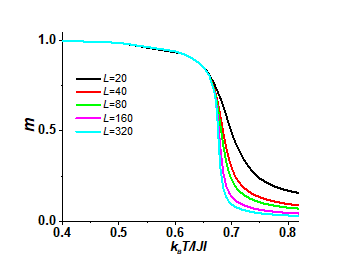
\includegraphics[width=\linewidth]{bab/image12.png}
        \caption{Температурная зависимость намагниченности $m$ для модели Поттса с $q=3$ на гексагональной решетке.}
        \label{fig:bab-2}
    \end{minipage}
    \hfill
    \begin{minipage}[c]{0.45\linewidth}
        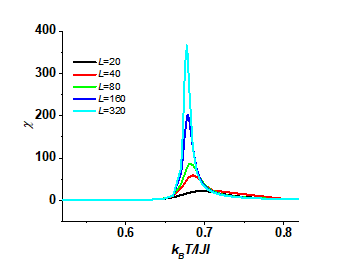
\includegraphics[width=\linewidth]{bab/image11.png}
        \caption{Температурная зависимость восприимчивости $\chi$ для модели Поттса с $q=3$ на гексагональной решетке.}
        \label{fig:bab-3}
    \end{minipage}
\end{figure}

На рисунках \ref{fig:bab-2} и \ref{fig:bab-3} представлены характерные зависимости намагниченности $m$ и 
восприимчивости $\chi$ для трехкомпонентной модели Поттса на гексагональной решетке от температуры соответственно. Здесь и далее на всех рисунках погрешность данных не превышает размеров символов, используемых для построения графиков. Как видно из этих рисунков, для всех рассмотренных систем наблюдается поведение характерное для фазового перехода второго рода.

В численных методах для определения температуры и рода ФП хорошо зарекомендовал метод кумулянтов Биндера четвертого порядка \cite{bib:bab-12}
\begin{gather}
    \label{eq:bab-6}
    V_L(T) = 1 - \frac{\left<E^4(T; L)\right>_L}{3\left<E^2(T; L)\right>_L^2}, \\
    \label{eq:bab-7}
    U_L(T) = 1 - \frac{\left<m^4\right>_L}{3\left<m^2\right>_{L^2}},
\end{gather}
где $E$ и $m$ -- энергия и намагниченность рассматриваемой системы с линейным размером $L$. Выражения \eqref{eq:bab-6} и \eqref{eq:bab-7} позволяют определить температуру $T_l$ фазового перехода с большой точностью в ФП первого и второго рода соответственно. Как известно ФП второго рода характеризуются следующими отличительными особенностями \cite{bib:bab-13}: усредненная величина $V_L(T)$ стремится к тривиальному значению $V^*$ согласно выражению
\begin{equation}
    \label{eq:bab-8}
    V(T) = V^* + bL^{-d}
\end{equation}
при $L \to \infty$ и $T=T_c(L)$, где $V^* = 2/3$, а кумулянты Биндера $U_L(T)$ в критической области имеют четко выраженную точку пересечения. Указанные особенности для кумулянтов Биндера четвертого порядка $V_L(T)$ и $U_L(T)$ продемонстрированы на рис.~\ref{fig:bab-4} и \ref{fig:bab-5} соответственно для ферромагнитной трехкомпонентной модели Поттса на гексагональной решетке. Методика определения рода фазового перехода этим методом подробно описана в работе \cite{bib:bab-14}. Как видно из рис.~\ref{fig:bab-4} температура ФП в трехкомпонентной модели Поттса на гексагональной решетке $T_c=0.673(2)$. Следует отметить, что для двумерных моделей Поттса с числом состояний спина $q$ из соображений дуальности квадратной, треугольной и гексагональной решетки были получены простые полиномиальные выражения, позволяющие определить критическую температуру (см. \cite{bib:bab-8}). Однако эти выражения справедливы только для моделей Поттса с $q>3$ и $q=2$ \cite{bib:bab-9}.
\begin{figure}[ht]
    \begin{minipage}[c]{0.45\linewidth}
        \includegraphics[width=\linewidth]{bab/image18.png}
        \caption{Температурная зависимость кумулянтов Биндера $V_L(T)$ для трехкомпонентной модели Поттса на гексагональной решетке.}
        \label{fig:bab-4}
    \end{minipage}
    \hfill
    \begin{minipage}[c]{0.45\linewidth}
        \includegraphics[width=\linewidth]{bab/image17.png}
        \caption{Температурная зависимость кумулянтов Биндера $U_L(T)$ для трехкомпонентной модели Поттса на гексагональной решетке.}
        \label{fig:bab-5}
    \end{minipage}
\end{figure}

Для рассмотренной модели Поттса на гексагональной решетке нами исследовалось критическое поведение на основе применения теории конечно-размерного скейлинга (КРС). Из соотношений этой теории следует, что для достаточно большой системы с ПГУ при температуре $T=T_c$ намагниченность $m$, восприимчивость $\chi$ удовлетворяют следующим аналитическим выражениям \cite{bib:bab-15}
\begin{gather}
    \label{eq:bab-9}
    m \sim L^{-\beta / v}, \\
    \label{eq:bab-10}
    \chi \sim L^{\gamma / v}.
\end{gather}

Эти соотношения были нами использованы для определения $\beta / v$ и $\gamma / v$. Для аппроксимации температурной зависимости теплоемкости от $L$ использовалось выражение
\begin{equation}
    \label{eq:bab-11}
    C = A + BL^{\alpha / v},
\end{equation}
где $A$, $B$ -- некоторые коэффициенты.

В соответствии с теорией КРС в точке ФП для критического индекса радиуса корреляции $v$ выполняется соотношение \cite{bib:bab-16}
\begin{equation}
    \label{eq:bab-12}
    v_n = L^{\frac{1}{v}} g_{v_n},
\end{equation}
где $g_{v_n}$ -- некоторая постоянная, а в качестве $V_n$ могут выступать:
\begin{equation}
    \label{eq:bab-13}
    V_i = \frac{\left<m^i E\right>}{\left<m^i\right>} - \left<E\right>, \quad (i = 1, 2, 3).
\end{equation}

Для расчета критических индексов (КИ) $\beta$, $\gamma$, $\alpha$, и $v$ строились зависимости $m$, $\chi$, $C$, и $V_n$ от $L$ (см. рис.~\ref{fig:bab-6}). Анализ данных, выполненный с использованием нелинейного метода наименьших квадратов, позволил определить значения $\beta / v$, $\gamma / v$, $\alpha / v$ и $1/v$ (см. Таблицу~\ref{tab:bab-1}). Затем, используя значения $v$, полученное в рамках данного исследования, определялись все остальные индексы $\beta$, $\gamma$, и $\alpha$. Точность критических индексов согласно выражениям теории КРС \eqref{eq:bab-9}-\eqref{eq:bab-12} в большей степени зависит от правильности учета данных для разных линейных размеров $L$. В наших расчетах строго контролировались данные для всех рассмотренных систем и при их незначительном отклонении от аппроксимирующей прямой процедура фитирования проводилась заново с отсеканием данных для $L<L_{\min}$. Такой отбор данных для разных линейных размеров $L$ позволяет заметно уменьшить погрешность в значениях КИ.
\begin{table}[ht]
    \centering
    \caption{Критические индексы для трехкомпонентной модели Поттса на гексагональной решетке}
    \label{tab:bab-1}
    \scriptsize
    \begin{tabular}{|p{2cm}*{9}{|c}|}
        \hline
        метод & $v$ & $1/v$ & $\alpha$ & $\alpha/v$ & $\gamma$ & $\gamma/v$ & $\beta$ & $\beta/v$ & $\alpha + 2\beta + \gamma = 2$ \\
        \hline
        Теория, \cite{bib:bab-9} & \makecell{5/6 \\ 0.83} & \makecell{6/5 \\ 1.20} & \makecell{1/3 \\ 0.333} & \makecell{2/5 \\ 0.40} & \makecell{13/9 \\ 1.444} & \makecell{26/15 \\ 1.733} & \makecell{1/9 \\ 0.111} & \makecell{2/15 \\ 0.133} & 2.0 \\
        \hline
        МК, гексагональная решетка (наши данные) & 0.847(3) & 1.180(2) & 0.327(3) & 0.387(3) & 1.446(1) & 1.708(3) & 0.107(3) & 0.127(3) & 1.99 \\
        \hline
        МК \cite{bib:bab-17}, квадратная решетка & & & & 0.46(8) & & 1.736(1) & & 0.131(1) & \\
        \hline
    \end{tabular}
    \medskip
\end{table}
\begin{figure}[ht]
    \begin{subfigure}{0.5\textwidth}
        \includegraphics[width=0.9\linewidth]{bab/image24.png}
    \end{subfigure}
    \begin{subfigure}{0.5\textwidth}
        \includegraphics[width=0.9\linewidth]{bab/image25.png}
    \end{subfigure}
    \begin{subfigure}{0.5\textwidth}
        \includegraphics[width=0.9\linewidth]{bab/image27.png}
    \end{subfigure}
    \begin{subfigure}{0.5\textwidth}
        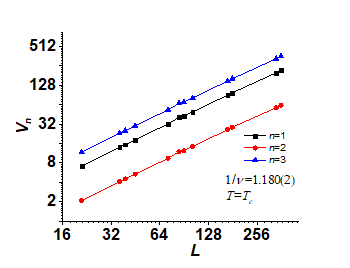
\includegraphics[width=0.9\linewidth]{bab/image26.png}
    \end{subfigure}
    \caption{Зависимость намагниченности $m$, восприимчивости $\chi$, теплоемкости $C$, для трехкомпонентной модели Поттса на гексагональной решетке от линейных размеров системы $L$ при $T = T_c$.}
    \label{fig:bab-6}
\end{figure}

\section*{Заключение}

Таким образом, полученные данные в результате компьютерного моделирования трехкомпонентной модели Поттса на гексагональной решетке свидетельствуют, что в ней наблюдается фазовый переход второго рода. При этом:
\begin{enumerate}
    \item Критическое поведение не демонстрирует мультипликативные логарифмические поправки к намагниченности, восприимчивости и теплоемкости, которые ранее были выявлены для модели Поттса с $q=4$ на квадратной решетке (см. работы, \cite{bib:bab-17,bib:bab-18}).
    \item Конечномерный анализ полученных данных демонстрирует наличие фазового перехода второго рода с критическими показателями (см. Табл.~\ref{tab:bab-1}), соответствующими классу универсальности модели Поттса с $q=3$ на квадратной решетке \cite{bib:bab-17}.
\end{enumerate}

\section*{Публикации}

\textbf{В центральных Российских изданиях:}
\begin{enumerate}
    \item Бабаев А.Б., Муртазаев А.К. Моделирование трехкомпонентной модели Поттса на гексагональной решетке методом Монте-Карло // Физика металлов и металловедение. -- 2023. -- Т.124. -- \textnumero 7. -- С. 577--583. \\ \url{https://www.sciencejournals.ru/view-article/?j=fizmet\&y=2023\&v=124\&n=7\&a=FizMet2360045Babaev}
\end{enumerate}

\textbf{В трудах международных и российских конференций:}
\begin{enumerate}
    \item Бабаев А.Б., Муртазаев А.К., Абуев Я.К., Ибаев Д.Г., Бабаев М.А. Исследование критического поведения трехкомпонентной модели Поттса на гексагональной решетке методом Монте-Карло // Сборник трудов международной конференции, посвященной 300-летию Российской академии наук -- 10-15 сентября 2023 г., Махачкала, С. 63--56.
\end{enumerate}

% NOTE: was in appendix
% \appendix

\section*{ПРАКТИЧЕСКОЕ ПРИМЕНЕНИЕ \\ АПРОБАЦИЯ ПОЛУЧЕННЫХ РЕЗУЛЬТАТОВ}

\textbf{Полученные нами результаты были представлены на следующих конференциях:}

Международная конференция, посвященная 300-летию Российской академии наук, 10-15 сентября 2023 г., Махачкала:
\begin{enumerate}
    \item Бабаев А.Б., Муртазаев А.К., Абуев Я.К., Ибаев Д.Г., Бабаев М.А. Исследование критического поведения трехкомпонентной модели Поттса на гексагональной решетке методом Монте-Карло (стендовый доклад Бабаева А.Б.)
\end{enumerate} 

\chapter{Об аппроксимативных свойствах рядов Фурье по полиномам Лагерра -- Соболева}

\section*{Введение}

Пусть $\alpha>-1$, $r\in \mathbb{N}$, $\rho(x)=e^{-x}x^\alpha$ -- весовая функция, $1\le p<\infty$, $L^p_\rho$ -- пространство измеримых функций $f$, определенных на полуоси $[0, \infty)$ и таких, что
$$
\|f\|_{L^p_\rho}=\left(\int\limits_0^{\infty}|f(x)|^p\rho(x) dx\right)^\frac{1}{p}<\infty,
$$
$W^r_{L^p_\rho}$ -- пространство функций $f$, непрерывно дифференцируемых $r-1$ раз, для которых $f^{(r-1)}$ абсолютно непрерывна на произвольном сегменте $[a, b]\subset[0, \infty)$, а $f^{(r)}\in L^p_\rho$.
Далее, через $W^r$ обозначим функции $f$ из $W^r_{L^2_\rho}$, для которых $|f^{(r)}(x)|e^{-\frac x2}\le 1$. В пространстве $W^r_{L^2_\rho}$ определим скалярное произведение типа Соболева
\begin{equation}\label{Gadzhimirzaev:SobInnerProd}
\langle f,g\rangle_S=\sum_{\nu=0}^{r-1}f^{(\nu)}(0)g^{(\nu)}(0)+\int_{0}^{\infty} f^{(r)}(x)g^{(r)}(x)\rho(x)dx.
\end{equation}

В работе~\cite{Gadzhimirzaev:DEMR2016} была введена система полиномов
\begin{equation*}
l_{r,r+n}^{\alpha}(x) =\frac{1}{(r-1)!\sqrt{h_n^\alpha}}\int\limits_{0}^x(x-t)^{r-1}L_{n}^{\alpha}(t)dt, \quad n=0,1,\ldots.
\end{equation*}
\begin{equation*}
l_{r,n}^{\alpha}(x) =\frac{x^n}{n!}, \quad n=0,1,\ldots, r-1,
\end{equation*}
ортонормированная при $\alpha>-1$ относительно скалярного произведения \eqref{Gadzhimirzaev:SobInnerProd} и порожденная системой полиномов Лагерра $\{L_{n}^{\alpha}(x)\}_{n=0}^\infty$.
В работе~\cite{Gadzhimirzaev:ShII-MMG} было показано, что система $\{l^\alpha_{r,k}(x)\}_{k=0}^\infty$ полна в $W^r_{L^2_\rho}$. Ряд Фурье функции $f\in W^r_{L^2_\rho}$ по этой системе имеет следующий вид
\begin{equation}\label{Gadzhimirzaev:Fourier_Series}
f(x)\sim \sum_{k=0}^{r-1}f^{(k)}(0)\frac{x^k}{k!}+\sum_{k=r}^{\infty} \hat{f}_{r,k}^\alpha l_{r,k}^\alpha(x),
\end{equation}
где
\begin{equation*}
\hat{f}_{r,k}^\alpha=\frac{1}{\sqrt{h_{k-r}^\alpha}}\int\limits_0^\infty f^{(r)}(t)L_{k-r}^\alpha(t)\rho(t)dt, \quad k\ge r.
\end{equation*}
В той же работе была доказана следующая

\textbf{Теорема A.}
\textit{
Пусть $-1<\alpha<1$, $f\in W^r_{L^2_\rho}$, $0\le A<\infty$. Тогда для произвольного $x\in [0,\infty)$ имеет место равенство
\begin{equation*}
f(x) = \sum_{k=0}^{r-1}f^{(k)}(0)\frac{x^k}{k!}+\sum_{k=r}^{\infty} \hat{f}_{r,k}^\alpha l_{r,k}^\alpha(x),
\end{equation*}
в котором ряд Фурье функции $f$ по полиномам $l_{r,k}^{\alpha}(x)$ сходится равномерно относительно $x\in[0,A]$.
}

Относительно параметра $p$ теорема \textbf{А} была обобщена в работе~\cite{Gadzhimirzaev:RamIzv2020}.

\textbf{Теорема B.}
\textit{
Пусть $-1<\alpha<1$. Тогда если $f\in W^r_{L^p_\rho}$, то при $p\ge2$ ряд \eqref{Gadzhimirzaev:Fourier_Series} сходится равномерно к $f$ на любом отрезке $[0,A]$. Если же $1\le p<2$, то существует функция $f\in W^r_{L^p_\rho}$, ряд Фурье которой расходится в точке $x=\pi^2$.
}

Рассмотрим случай, когда $\alpha=0$. В этом случае для полиномов $l_{r,r+n}^{0}(x)$ имеет место равенство~\cite[следствие 3.1]{Gadzhimirzaev:ShII-MMG}:
\begin{equation*}
l_{r,r+n}^{0}(x)=\frac{x^r L_n^r(x)}{(n+r)^{[r]}},
\end{equation*}
где $(n+r)^{[r]}=(n+r)(n+r-1)\ldots(n+1)$.
Тогда ряд Фурье \eqref{Gadzhimirzaev:Fourier_Series} примет следующий вид
\begin{equation*}
f(x)\sim \sum_{\nu=0}^{r-1}f^{(\nu)}(0)\frac{x^k}{k!}+x^r\sum_{k=0}^{\infty} \frac{\hat{f}_{r,k+r}^0}{(k+r)^{[r]}}L_k^r(x).
\end{equation*}
Частичную сумму этого ряда обозначим через $S_{r,n+r}(f,x)$:
\begin{equation}\label{Gadzhimirzaev:part-sum}
S_{r,n+r}(f,x)=\sum_{\nu=0}^{r-1}f^{(\nu)}(0)\frac{x^k}{k!}+x^r\sum_{k=0}^{n} \frac{\hat{f}_{r,k+r}^0}{(k+r)^{[r]}}L_k^r(x).
\end{equation}
Из \eqref{Gadzhimirzaev:part-sum} следует, что для $S_{n+r}(f,x)$ имеют место равенства
\begin{equation*}
S_{r,n+r}^{(\nu)}(f,0)=f^{(\nu)}(0), \quad 0\le\nu\le r-1.
\end{equation*}
Кроме того, если $f(x)=p_{n+r}(x)$ -- алгебраический полином степени $n+r$, то
\begin{equation}\label{Gadzhimirzaev:part-sum-second-prop}
S_{r,n+r}(p_{n+r},x)\equiv p_{n+r}(x).
\end{equation}

Используя свойство \eqref{Gadzhimirzaev:part-sum-second-prop}, авторы работы \cite{Gadzhimirzaev:ShII-MMG} исследовали аппроксимативные свойства частичных сумм $S_{r,n+r}(f,x)$. В частности, для $f\in W^r_{L^2_\omega}$, $\omega(x)=e^{-x}$ было показано,
что имеет место неравенство типа Лебега~\cite[теорема 5.2]{Gadzhimirzaev:ShII-MMG}
$$
e^{-x/2}x^{-r/2+1/4}|f(x)-S_{r,n+r}(f,x)|\le (1+\lambda_{r,n}(x))E_{n+r}^r(f),
$$
в котором для функции $\lambda_{r,n}(x)$ справедливы оценки
$$
\lambda_{r,n}(x)\le c(r)
\begin{cases}
	\ln(n+1), & x\in[0,\kappa/2]; \\
	\ln(n+1)+(x/(\kappa^{1/3}+|x-\kappa|))^{1/4}, & x\in[\kappa/2,3\kappa/2]; \\
	n^{-r/2+5/4}e^{-x/4}, & x\in[3\kappa/2,\infty).
\end{cases}
$$
Здесь $c(r)$ положительная константа, зависящая только от $r$, $\kappa=4n+2r+2$.
Величина $E_{n+r}^r(f)$ определяется равенством
$$
E_{n+r}^r(f)=\inf_{q_{n+r}}\sup_{x>0}|q_{n+r}(x)-f(x)|e^{-x/2}x^{-r/2+1/4},
$$
где нижняя грань берется по всем алгебраическим полиномам $q_{n+r}$ степени $n+r$, для которых $f^{(\nu)}(0)=q_{n+r}^{(\nu)}(0)$, $\nu=\overline{0,r-1}$.

Вышеприведенные оценки для разности $|f(x)-S_{r,n+r}(f,x)|$ содержат величину наилучшего приближения $E_{n+r}^r(f)$, поведение которой все еще не исследовано. В этом разделе для случая $r=1$ получена оценка скорости сходимости частичных сумм $S_{1,n+1}(f,x)$ к функции $f(x)$, не содержащая величины наилучшего приближения $E_{n+r}^r(f)$.

Аналогичные задачи о приближении функций из пространства Соболева алгебраическими полиномами были исследованы в работах различных авторов
(см. \cite{Approx-Xu}--\cite{Approx-Leonardo} и цитированную в них литературу). В частности, в \cite{Approx-Xu} при $1\le p<\infty$ было рассмотрено пространство $W^r_{L^p_w}=W^r_{L^p_w}[-1,1]=\{f\in C^{r-1}[-1,1]: f^{(r)}\in L^p_w\}$, $w(x)=w_{\alpha,\beta}(x)=(1-x)^\alpha(1+x)^\beta$ с нормой
$$
\|f\|_{W^r_{L^p_w}}=\left(\sum_{k=0}^{r}\|f^{(k)}\|^p_{L^p_w}\right)^{1/p}.
$$
Для функций из этого пространства были доказаны следующие теоремы.

\textbf{Теорема C.}
\textit{
Пусть $\alpha,\beta>-1$. Предположим, что $f\in W^r_{L^p_w}$ при $1\le p<\infty$ или $f\in C^r[-1,1]$ при $p=\infty$. Тогда существует полином $p_n$ такой, что
$$
\|f-p_n\|_{W^r_{L^p_w}}\le c E_n(f^{(r)})_{L^p_w},
$$
где $E_n(f^{(r)})_{L^p_w}=\inf\limits_{p\in\Pi_n}\|f^{(r)}-p\|_{L^p_w}$ -- величина наилучшего приближения в метрике $L^p_w$.
}

\textbf{Теорема D.}
\textit{
Пусть $\alpha,\beta>-1$. Предположим, что $f\in W^r_{L^p_w}$ при $1\le p<\infty$ или $f\in C^r[-1,1]$ при $p=\infty$. Тогда существует полином $p_n$ такой, что
$$
\|f^{(k)}-p_n^{(k)}\|_{L^p_w}\le c n^{-r+k}E_n(f^{(r)})_{L^p_w}
$$
при условии, что либо $\alpha=0$, либо $\beta=0$.
}

Далее, в работе \cite{Approx-Juan} было рассмотрено пространство $H^r_\omega=H^r_\omega(a,b)=\{f\in L^2_\omega(a,b): f^{(m)}\in L^2_\omega(a,b), 1\le m\le r\}$ с нормой
$$
\|f\|_{H^r_\omega}=\left(\sum_{m=0}^{r}\|f^{(m)}\|^2_{L^2_w}\right)^{1/2}.
$$
Здесь $(a, b)=\mathbb{R}$ при $\omega(x)=e^{-x^2}$, $(a,b)=(0, \infty)$ при $\omega(x)=e^{-x}x^\alpha$, $\alpha>-1$ и $(a,b)=(-1, 1)$ при $\omega(x)=(1-x)^\alpha(1+x)^\beta$, $\alpha, \beta>-1$.
Был исследован вопрос о приближении функций из этого пространства в метрике $L^2_\omega$ посредством частичных сумм $\mathcal{S}_n^Nf(x)$ ряда Фурье по системе полиномов $\{q_j(x)\}$, ортогональной относительно скалярного произведения Соболева. А именно, была доказана следующая

\textbf{Теорема E.}
\textit{
Пусть $r\ge N+1$ и функция $f\in H^r_\omega$ такая, что $f\in L^2_{v_{r-N-1}}$. Тогда оценки
$$
\|f^{(m)}-(\mathcal{S}_n^Nf)^{(m)}\|_{L^2_\omega}\le c
\begin{cases}
\frac{(-\lambda_{n-N,0})^{(m-N)/2}}{(-\lambda_{n-r,r-N-1})^{(r-N-1)/2}}E_{n-r}(f^{(r)})_{L^2_{v_{r-N-1}}}, N\le m\le r, \\
\frac{(-\lambda_{n-N,0})^{N/2}}{(-\lambda_{n-r,r-N-1})^{(r-N-1)/2}}E_{n-r}(f^{(r)})_{L^2_{v_{r-N-1}}}, 0\le m\le N-1,
\end{cases}
$$
выполняются всегда в случае весовой функции Эрмита, для $\alpha>-1$ в случае весовой функции Лагерра и при $\alpha, \beta\ge0$ в случае весовой функции Якоби.
}

\section{Некоторые сведения о полиномах Лагерра}

Пусть $\alpha$ произвольное действительное число. Тогда для полиномов Лагерра $L_n^\alpha(x)$ справедливы следующие соотношения~\cite{Gadzhimirzaev:Szego}:
\begin{itemize}
\item
формула Родрига
$$
L_n^\alpha(x)=\frac{1}{n!}x^{-\alpha}e^x\left(x^{n+\alpha}e^{-x}\right)^{(n)};
$$

\item
соотношение ортогональности
$$
\int_{0}^{\infty}L_n^\alpha(x)L_m^\alpha(x)\rho(x)dx=h_n^\alpha\delta_{n,m},\ \alpha>-1,
$$
где $\delta_{n,m}$ -- символ Кронекера, $h_n^\alpha=\frac{\Gamma(n+\alpha+1)}{\Gamma(n+1)}$;
\item
формула Кристоффеля -- Дарбу
\begin{equation*}\label{Gadzhimirzaev:Darbu}	
K_n^\alpha(x,t)=\sum_{k=0}^{n}\frac{L_k^\alpha(x)L_k^\alpha(t)}{h_k^\alpha}=
\frac{n+1}{h_n^\alpha}\frac{L_n^\alpha(x)L_{n+1}^\alpha(t)-L_{n+1}^\alpha(x)L_n^\alpha(t)}{x-t};
\end{equation*}

\item
рекуррентная формула
$$
L_0^\alpha(x)=1, \ L_1^\alpha(x)=-x+\alpha+1,
$$
\begin{equation*}\label{Gadzhimirzaev:recur}
nL_n^\alpha(x)=(-x+2n+\alpha-1)L_{n-1}^\alpha(x)-(n+\alpha-1)L_{n-2}^{\alpha}(x), \ n\ge2;
\end{equation*}

\item
равенства
\begin{equation*}\label{Gadzhimirzaev:prop1}
nL_n^\alpha(x)=(n+\alpha)L_{n-1}^\alpha(x)-xL_{n-1}^{\alpha+1}(x),
\end{equation*}
\begin{equation*}\label{Gadzhimirzaev:prop2}
L_n^{\alpha-1}(x)=L_{n}^\alpha(x)-L_{n-1}^{\alpha}(x);
\end{equation*}

\item
весовая оценка~\cite{Gadzhimirzaev:AskeyWain,Gadzhimirzaev:Mocken}
\begin{equation*}\label{Gadzhimirzaev:weight-est}
e^{-\frac{x}{2}}|L_n^\alpha(x)|\le c(\alpha)A_n^\alpha(x),\ \alpha>-1.
\end{equation*}
\end{itemize}
Здесь и далее $c$, $c(\alpha)$ -- положительные числа, зависящие от указанных параметров,
$$
A_n^\alpha(x)=
\begin{cases}
	\theta^\alpha, & 0\le x\le \frac{1}{\theta}; \\
	\theta^{\frac{\alpha}{2}-\frac14}x^{-\frac{\alpha}{2}-\frac14}, & \frac{1}{\theta}< x\le \frac{\theta}{2}; \\
	\left[\theta\left(\theta^{\frac13}+|x-\theta|\right)\right]^{-\frac14}, & \frac{\theta}{2}< x\le \frac{3\theta}{2}; \\
	e^{-\frac x4}, & \frac{3\theta}{2}<x,
\end{cases}
$$
где $\theta=\theta_n(\alpha)=4n+2\alpha+2$.

Для ортонормированных полиномов Лагерра $l_n^\alpha(x)=\frac{1}{\sqrt{h_n^\alpha}}L_n^\alpha(x)$ имеют место оценки
\begin{equation*}\label{Gadzhimirzaev:orth-est}
e^{-\frac{x}{2}}|l_{n+1}^\alpha(x)-l_{n-1}^\alpha(x)|\le c(\alpha)
\begin{cases}
		\theta^{\frac{\alpha}{2}-1}, & 0\le x\le \frac{1}{\theta}; \\
		\theta^{-\frac34}x^{-\frac{\alpha}{2}+\frac14}, & \frac{1}{\theta}< x\le \frac{\theta}{2}; \\
		x^{-\frac{\alpha}{2}}\theta^{-\frac34}\left(\theta^{\frac13}+|x-\theta|\right)^{\frac14}, & \frac{\theta}{2}< x\le \frac{3\theta}{2}; \\
		e^{-\frac x4}, & \frac{3\theta}{2}<x.
\end{cases}
\end{equation*}

\section{Вспомогательные утверждения и основной результат}

Пусть $\mathcal{K}_{n}(x,t)=\sum\limits_{k=0}^{n}L_k^1(x)L_k(t)$. Справедливы следующие утверждения.

\begin{lemma}
Имеет место равенство
\begin{equation*}\label{Gadzhimirzaev:ker}
(x-t)\mathcal{K}_{n}(x,t)=(n+1)\left(L^1_{n}(x)L_{n+1}(t)-L^1_{n+1}(x)L_{n}(t)\right)+\sum_{k=0}^{n}L_{k}(x)L_{k}(t).
\end{equation*}
\end{lemma}

\begin{lemma}
Для величины $\mathcal{K}_{n}(x,t)$ справедливо равенство
\begin{equation*}
(x-t)\mathcal{K}_{n}(x,t)=xL^2_{n}(x)L_{n}(t)-tL^1_{n}(x)L^1_{n}(t)-L^1_{n}(x)L_{n}(t)+\sum_{k=0}^{n}L_{k}(x)L_{k}(t).
\end{equation*}
\end{lemma}

\begin{lemma}
Для $K_{n}^0(x,t)=\sum\limits_{k=0}^{n}L_{k}(x)L_{k}(t)$ имеет место представление
$$
K_n^0(x,t)=\frac{n+1}{2n+1}L_{n}(x)L_{n}(t)+
$$
\begin{equation*}	
\frac{n(n+1)}{2n+1}\frac{1}{t-x}\left[L_{n}(t)\left(L_{n+1}(x)-L_{n-1}(x)\right)-L_{n}(x)\left(L_{n+1}(t)-L_{n-1}(t)\right)\right].
\end{equation*}
\end{lemma}

\begin{lemma}
Имеет место равенство
\begin{equation*}
\sum_{k=0}^{\infty}\left(\frac{x^{\frac34}L_k^1(x)}{k+1}\right)^2 = \frac{e^{x}-1}{\sqrt{x}}, \ x\in[0,\infty).
\end{equation*}
\end{lemma}

\begin{lemma}
\cite{Gadzhimirzaev:mathnot2021}	
Пусть $\alpha>-1$, $n\in\mathbb{N}$, $x\in[0,\infty)$. Тогда имеют место следующие оценки
\begin{equation*}
e^{-x}K_{n}^\alpha(x,x)\le c(\alpha)
\begin{cases}
n^{-\alpha}, & x\in[\theta_n/2, 3\theta_n/2], \\
n^{1-\alpha}(A_n^\alpha(x))^2, & x\in[0,\theta_n/2]\cup[3\theta_n/2,\infty).
\end{cases}
\end{equation*}
\end{lemma}

Основным результатом этого раздела является следующая
\begin{theorem}\label{Gadzhimirzaev:theorem1}
Пусть $f\in W^1$, $x\in[0,\infty)$. Тогда имеет место оценка
$$
\frac{x^{-\frac14}e^{-\frac x2}}{\sqrt{x+1}}|f(x)-S_{1,n+1}(f,x)|\le c
\frac{\ln(n+1)}{n^{\frac14}},
$$
где $c$ -- положительная константа.
\end{theorem}


\chapter{Краткая аннотация важнейших и основных научных результатов,
полученных в 2022 г.}

\begin{enumerate}

\item Изучены вопросы моментной устойчивости решений по части
переменных относительно начальных данных для систем линейных
дифференциальных уравнений Ито с последействием. Исследование
проводится модифицированным методом регуляризации, основанным на
выборе вспомогательного уравнения и применении теории неотрицательно
обратимых матриц. Для упомянутых систем получены достаточные условия устойчивости в терминах неотрицательной обратимости матриц,
построенных по параметрам этих систем. Проверяется выполнимость этих
условий для конкретных классов систем линейных уравнений Ито с
последействием. Результаты исследований опубликованы в работах 

\item Исследована глобальная моментная устойчивость систем
дифференциальных уравнений Ито дробного порядка с последествием. Для
этого применяется метод регуляризации в качестве альтернативы
алгоритмам, основанных на функционалах Ляпунова. Центральная идея
этого метода основана на параллелизме между устойчивостью по
Ляпунову и стохастической версией устойчивости по входным данным,
которая хорошо известна в теории управления детерминированными
обыкновенными дифференциальными уравнениями. Первый шаг алгоритма
состоит в преобразовании заданного уравнения с последествием в
функционально-дифференциальное уравнение Ито дробного порядка со
стохастическим управлением и тем самым заменяя устойчивость по
Ляпунову первого уравнения устойчивостью  второго по входному
состоянию. Для оценки норм решений функционально-дифференциального
уравнения Ито дробного порядка мы используем метод регуляризации,
основанный на концепции положительно обратимых матриц. Эффективность
этого метода демонстрируется с помощью некоторых примеров, где метод
функционалов Ляпунова может быть труден в применении. 

\item Изучено  асимптотическое поведение моментов решений систем
нелинейных дифференциальных уравнений Ито с запаздываниями. Эти
вопросы тесно связаны с вопросами глобальной моментная устойчивости
этих же систем. Исследования проведены модифицированным методом
регуляризации (W-метод), основанный на выборе вспомогательного
уравнения и применении теории положительно обратимых матриц.
Получены достаточные условия, обеспечивающие наличие определенного
асимптотического поведения для моментов решений как для достаточно
общих, так и конкретных классов уравнений Ито в терминах параметров
этих классов. Установлена связь между асимптотическим поведением
моментов решений для упомянутых систем и запаздываниями. 

\end{enumerate}

\section*{Введение}

Стохастические дифференциальные уравнения
описывают многие реальные, практически важные процессы современной
физики, биологии, иммунологии, экономики, кибернетики и т.д.
Изучение таких процессов привело к необходимости исследований
вопросов устойчивости решений стохастических дифференциальных
уравнений, т.е. к созданию соответствующего направления в теории
устойчивости.

Математические модели многих реальных процессов, учитывающие
состояния процессов не только в текущий, но и в предшествующие
моменты времени описывают развитие процессов более точнее. В этом
случае поведение процесса, подверженного случайным воздействиям,
описывается стохастическими дифференциальными уравнениями с
последействием. Примеры показывают, что поведение решений уравнений
без учета запаздывания, даже при малой его величине, может
существенно отличаться от поведения решений тех же уравнений с
запаздывающим аргументом. Это обстоятельство подчеркивает
необходимость и принципиальную важность изучения уравнений с учетом
запаздывания.

Вопросам устойчивости решений систем со случайными параметрами
посвящено большое количество работ как отечественных, так и
зарубежных математиков. Достаточно полный их список приведен в
монографиях. Исследования устойчивости в этих и многих других
работах проводятся методом функционалов
Ляпунова\-/Красовского\-/Разумихина. Этот метод предполагает
существование подходящей функции Ляпунова (функционала
Ляпунова\-/Красовского), которая обеспечивает желаемое свойство
устойчивости (асимптотического поведения) решений исследуемых
уравнений. Однако применение этого метода для
функционально\-/дифференциальных уравнений, частным случаем которых
являются дифференциальные уравнения с отклоняющим аргументом, во
многих случаях встречает серьёзные трудности. В теории устойчивости
решений для детерминированных функционально\-/дифференциальных
уравнений широкое применение и высокую эффективность показал метод
регуляризации, основанный на выборе вспомогательных или <<модельных>> уравнений  --- <<W--метод>> Н.В. Азбелева.

Исследованиям проблем устойчивости  по части переменных  решений для
детерминированных динамических систем и их приложениям посвящены
много работ. Главной целью исследований за отчетный период является
развитие метода вспомогательных уравнений на основе теории
неотрицательно обратимых матриц и покомпонентных оценок решений
применительно к исследованию вопросов моментной устойчивости решений
по части переменных для систем линейных дифференциальных уравнений
Ито с последействием относительно начальных данных. Этот подход
ранее показал свою эффективность при исследовании вопросов
устойчивости решений для систем линейных дифференциальных уравнений
Ито с последействием и, как показано в настоящем отчете, позволяет
получить новые, конструктивные результаты устойчивости решений по
части переменных относительно начальных данных для детерминированных
и стохастических систем с запаздываниями и без него.

\section{Постановка задачи}\label{sec:kri-1}

В отчете используются
следующие обозначения:
\begin{itemize}
    \item $(\Omega , {\mathcal F}, ({\mathcal
    F})_{t\ge0},P)$ --- стохастический базис, здесь $ \Omega $ ---
    множество
    элементарных событий, ${\mathcal F}$ --- $\sigma$--алгебра событий на
    $\Omega$,  $({\mathcal F})_{t\ge 0}$ --- непрерывный справа неубывающий поток
    $\sigma$--подалгебр алгебры ${\mathcal F}$, $P$ --- вероятностная
    мера на ${\cal F}$, и  все $\sigma$--алгебры являются полными относительно этой
    меры;
    \item $k^n$ --- линейное пространство $n$--мерных ${\mathcal F}_0$ ---
    измеримых случайных величин;
    \item $\mathcal B_i,i=2,\dots,m$ --- скалярные независимые стандартные
    винеровские процессы;
    \item  $E$ --- символ математического
    ожидания;
    \item $\bar E$ -- единичная $k \times k$--матрица;
    \item  $|.|$ --- норма в $R^n$;
    \item $||.||$
    --- норма $k\times n$--матрицы, согласованная с нормой в $R^n$;
    \item $\mu$ --- мера Лебега на $[0,\infty)$.
\end{itemize}


В рамках отчета следующие константы также остаются фиксированными:
\begin{itemize}
    \item $n \in N$ --- размерность фазового пространства уравнения, т.е. размер вектора решения уравнения;
    \item $p$ --- фиксированная вещественная константа, $1 \le  p < \infty $;
    \item $q$ --- фиксированная вещественная константа, $1 \le  q < \infty $;
    \item $l$ --- фиксированное натуральное число такое, что $1 \le  l < n$.
\end{itemize}

За отчетный период были исследованы вопросы моментной устойчивости
решений по части переменным для системы линейных дифференциальных
уравнений Ито с запаздываниями вида
\begin{equation}
\label{eq:kri-1}
\begin{array}{crl}
dx(t) = - \sum \limits_{j=1}^{m_1}A_{1j}(t)x(h_{1j}(t))dt + \sum
\limits_{i=2}^m\sum
\limits_{j=1}^{m_i}A_{ij}(t)x(h_{ij}(t))d\mathcal B_i(t) \, (t \ge
0)
\end{array}
\end{equation}
относительно начальных данных
\begin{gather}
\label{eq:kri-1a}
x(t) = \varphi(t) \quad (t <0), \quad   
\\
\label{eq:kri-1b}
x(0) = \upsilon,  
\end{gather}
где:
\begin{enumerate}
    \item $x = col(x^1,\dots,x^n)$ --- $n$--мерный неизвестный случайный
    процесс;
    
    \item  $A_{ij} = (a^{ij}_{sl})^n_{s,l=1}$ --- $n \times n$--матрица при
    $i = 1,\dots,m$, $j = 1,\dots,m_i$, элементами матриц $A_{1j}$, $j =
    1,\dots,m_1$ являются прогрессивно измеримые скалярные случайные
    процессы, траектории которых почти наверно (п.н.) локально
    суммируемы, а элементами матриц $A_{ij}$, $i = 2,\dots,m$, $j =
    1,\dots,m_i$ являются прогрессивно измеримые скалярные случайные
    процессы, траектории которых п.н. локально суммируемы с квадратом;
    
    \item  $ h_{ij}$ --- измеримая по Борелю функция, заданная на $[0,
    \infty)$ такая, что $ h_{ij}(t)\leq t {\,} {\,} (t \in [0, \infty))$
    $\mu $--почти всюду при $i = 1,\dots,m$, $j = 1,\dots,m_i$;
    
    \item  $\varphi = col (\varphi _1,\dots, \varphi _n)$ --- ${\mathcal
    F}_0$--измеримый $n$--мерный случайный процесс, заданный на
    $(-\infty , 0)$;
    
    \item  $\upsilon = col (\upsilon_1,.., \upsilon_n)$ --- ${\mathcal
    F}_0$--измеримая $n$--мерная случайная величина, т.е. $\upsilon \in
    k^n$.
\end{enumerate}

\begin{definition}\label{def:kri-1}
    Под решением системы \eqref{eq:kri-1}, удовлетворяющим
    начальным условиям \eqref{eq:kri-1a} и \eqref{eq:kri-1b}, понимается случайный процесс $x(t) =
    col (x^1(t), \dots, x^n(t))$ $ (t \in (-\infty , \infty))$,
    прогрессивно измеримый при  $t \ge 0$, удовлетворяющий условиям
    $x(\varsigma)=\varphi (\varsigma) {\,} (\varsigma < 0)$, $x(0) =
    \upsilon$ и системе
    $$
    \begin {array}{crl}
     x(t) =   \upsilon - \sum \limits_{j=1}^{m_1}\int \limits _0^t A_{1j}(\varsigma)x(h_{1j}(\varsigma))d\varsigma
     + \sum \limits_{i=2}^m\sum
    \limits_{j=1}^{m_i}\int \limits
     _0^t A_{ij}(\varsigma)x(h_{ij}(\varsigma))d\mathcal B_i(\varsigma)
     \,\, (t \ge 0)
    \end {array}
    $$
    $P$--почти всюду, где первый интеграл --- интеграл Лебега, а второй
    --- интеграл Ито.
\end{definition}

Систему \eqref{eq:kri-1} с условиями \eqref{eq:kri-1a} и \eqref{eq:kri-1b} называют начальной задачей, а
условия \eqref{eq:kri-1a}, \eqref{eq:kri-1b} --- начальными условиями. Если $h_{ij}(t) = t$
$(t \geq 0)$  $\mu $--почти всюду при $i = 1,\dots,m$, $j =
1,\dots,m_i$, то условие \eqref{eq:kri-1a} лишнее. В этом случае \eqref{eq:kri-1}, \eqref{eq:kri-1b} называют
задачей Коши для системы линейных дифференциальных уравнений Ито.

Пусть в дальнейшем:
\begin{itemize}
    \item $D^n$ --- линейное пространство $n$--мерных прогрессивно измеримых
    случайных процессов на $[0, \infty )$, траектории которых п.н.
    непрерывны;
    
    \item $L^n$ --- линейное пространство $n$--мерных случайных процессов на
    $(-\infty , 0)$, которые не зависят от винеровских процессов
    $\mathcal B_i, i = 2, \dots, m$ и имеют п.н. ограниченные в
    существенном траектории;
    
    \item $\gamma :[0, \infty) \rightarrow R^1 $
\end{itemize}
--- положительная непрерывная функция.

Отметим, что при сделанных предположениях задача \eqref{eq:kri-1}, \eqref{eq:kri-1a}, \eqref{eq:kri-1b}
имеет единственное решение. Обозначим через $x(t, \upsilon,
\varphi)$ $(t \in (-\infty , \infty ))$ решение системы \eqref{eq:kri-1},
удовлетворяющее условиям \eqref{eq:kri-1a} и \eqref{eq:kri-1b}, т.е. $x(t, \upsilon, \varphi )
= \varphi (t)$ при $t < 0$ и $x(0, \upsilon, \varphi ) = \upsilon$.
Очевидно, что при $t \ge 0$ имеем $x(., \upsilon, \varphi) \in D^n$.
Заметим также, что при нулевых начальных условиях \eqref{eq:kri-1a}, \eqref{eq:kri-1b} задача
\eqref{eq:kri-1}, \eqref{eq:kri-1a}, \eqref{eq:kri-1b} имеет только тривиальное решение.

Для любого $x = col (x^1, \dots, x^n)$ введем обозначения $y =  col
(x^1, \dots, x^l)$ и \\$\xi = col (x^{l+1                   }, \dots,
x^n)$.

Введем также обозначения для следующих линейных нормированных
подпространств пространств $D^l$, $k^n$, $L^n$:

$ M_q^{\gamma } = \left \{x: x \in D^l, ||x||_{M_q^\gamma }
 \mathrel
 {\mathop {=} \limits ^{def}} \mathrel {\mathop {\sup}
 \limits _{t
 \ge 0}} (E|\gamma (t)x(t)|^q)^{1/q} < \infty \right \}  (
 M_q^1 = M_q)$;

$ k_q^n = \left \{\alpha: \alpha \in k^n, ||\alpha ||_{k_q^n}
 \mathrel
 {\mathop {=} \limits ^{def}} (E|\alpha |^q)^{1/q} < \infty
 \right  \}$;

 $L_q^n = \left \{\varphi: \varphi \in L^n,
 ||\varphi||_{L_q^n}
 \mathrel {\mathop {=} \limits ^{def}} \mathrel {\mathop
 {vrai \sup}
 \limits _{\varsigma < 0}}(E|\varphi (\varsigma ) |^q)^{1/q} < \infty
 \right \}$.


\begin{definition}\label{def:kri-2}
    Тривиальное решение $x(t,0, 0)\equiv 0$
    системы \eqref{eq:kri-1} (или систему \eqref{eq:kri-1}) назовем:
    
    \begin{itemize}
        \item {\it $q$--устойчивым} относительно первых $l$ компонент, если
        для любого $\epsilon > 0$ найдется такое $\delta (\epsilon) > 0$,
        что при любых $\upsilon \in k^n_q$, $\varphi \in L^n_q$ и
        $\|\upsilon\|_{k^n_q} + \|\varphi \|_{L^n_q} < \delta (\epsilon)$
        будет выполнено неравенство $(E|y(t,\upsilon, \varphi)|^q)^{1/q} \le
        \epsilon $ для любого $t \ge 0$;
        
        \item {\it асимптотически $q$--устойчивым }относительно первых $l$ компонент, если
        оно $q$\-/устойчиво, и, кроме того, для любых $\upsilon \in
        k^n_q$, $\varphi \in L^n_q$ и $\|\upsilon\|_{k^n_q} + \|\varphi
        \|_{L^n_q} < \delta (\epsilon)$ будет $\lim \limits_{t  \rightarrow
        +\infty }(E|y(t,\upsilon, \varphi)|^q)^{1/q}$ $ = 0$;
        
        \item {\it экспоненциально $q$--устойчивым }относительно первых $l$ компонент, если
        существуют некоторые положительные числа $\bar c, \beta$ такие, что
        для любых $\upsilon \in k^n_q$, $\varphi \in L^n_q$ справедливо
        неравенство $(E|y(t,\upsilon, \varphi)|^q)^{1/q} \le \bar
        c\left(\|\upsilon\|_{k^n_q} + \|\varphi \|_{L^n_q}\right)\exp
        \{-\beta t\}$.
    \end{itemize}
\end{definition}

Следующее определение объединяет все виды устойчивости из
Определения~\ref{def:kri-2}.

\begin{definition}\label{def:kri-3}
    Систему \eqref{eq:kri-1} назовем  $M_q^\gamma y
    $--устойчивым, если для любых $\upsilon \in k^n_q$, $\varphi \in
    L^n_q$ для решения задачи \eqref{eq:kri-1}, \eqref{eq:kri-1a}, \eqref{eq:kri-1b}   $x(t,\upsilon,
    \varphi)(t \in (-\infty, +\infty))$ выполняются  соотношение $y(.,
    \upsilon, \varphi)|_{[0,\infty)} \in M_q^\gamma$ и неравенство
    \begin{equation}
        \label{eq:kri-2}
        \|y(., \upsilon, \varphi)|_{[0,\infty)}\|_{M_q^\gamma} \le \bar c\left(\|\upsilon\|_{k^n_q} +
        \|\varphi \|_{L^n_q}\right)
    \end{equation}
    для некоторого положительного числа $\bar c$.
\end{definition}

Очевидно, что:
\begin{itemize}
    \item из  $M_qy$--устойчивости системы \eqref{eq:kri-1}
    следует $q$--устойчивость этой же системы относительно  первых $l$
    компонент;
    
    \item из $M_q^\gamma y$--устойчивости системы \eqref{eq:kri-1}
    (где $\gamma (t) \ge \delta > 0$ $(t \ge 0)$ и $\lim \limits _{t
    \rightarrow +\infty } \gamma (t) = +\infty )$ следует
    асимптотическая $q$--устойчивость этой же системы относительно
    первых $l$ компонент;
    
    \item из $M_q^\gamma y$--устойчивости системы \eqref{eq:kri-1}
    (где $\gamma (t) = \exp \{\beta t\}$, $\beta$ --- некоторое
    положительное число) следует экспоненциальная $q$--устойчивость этой
    же системы относительно первых $l$ компонент.
\end{itemize}


Для установления $M_q^\gamma y$--устойчивости системы \eqref{eq:kri-1} необходимо
проверить принадлежность вектора $y(., \upsilon,\varphi
)|_{[0,\infty)}$ составленный из первых $l$ компонент решения задачи
\eqref{eq:kri-1}, \eqref{eq:kri-1a}, \eqref{eq:kri-1b} $x(t,\upsilon, \varphi)(t \in (-\infty, +\infty))$
пространству $M_q^\gamma$ при любых $\upsilon \in k^n_q$, $\varphi
\in L^n_q$ и выполнимость для него неравенства \eqref{eq:kri-2}. Для этого будет
использована модификация метода вспомогательных  или модельных
уравнений, известная также как $W$--метод, основанная на теории
положительно обратимых матриц и покомпонентных оценках решений.

\section{Метод исследования}\label{sec:kri-2}

Как было отмечено ранее,
устойчивость системы \eqref{eq:kri-1} относительно первых $l$ компонент будем
проверять преобразованием этой системы с помощью вспомогательной
(модельной) системы в другую, более простую систему, для которой
условия, обеспечивающие устойчивость системы \eqref{eq:kri-1} относительно первых
$l$ компонент можно проверить непосредственно.

В дальнейшем будем пользоваться следующим представлением для решения
задачи \eqref{eq:kri-1}, \eqref{eq:kri-1a}, \eqref{eq:kri-1b}: $x(t) = \bar x(t) + \bar \varphi (t)$, где
$\bar x(t)$ --- неизвестный $n$--мерный случайный процесс на
$(-\infty, \infty)$ такой, что $\bar x(t) = 0$ при $t < 0$ и $\bar
x(t) = x(t)$ при $t \geq 0$,  а $\bar  \varphi (t)$ --- известный
$n$--мерный случайный процесс на $(-\infty, \infty)$ такой, что
$\bar \varphi(t) = \varphi (t)$ при $t < 0$ и $\bar \varphi(t) = 0$
при $t \geq 0$.  Тогда  задача \eqref{eq:kri-1}, \eqref{eq:kri-1a}, \eqref{eq:kri-1b} эквивалентна
следующей задаче
\begin{gather}
    \label{eq:kri-3}
    d\bar x(t) =  ((V\bar x)(t) +f(t))dZ(t) {\,} (t \ge 0),
    \\
    \label{eq:kri-3b}
    \bar x(0) = \upsilon,  
\end{gather}
где
\begin{align*}
    &(V\bar x)(t)= \left(- \sum \limits_{j=1}^{m_1}A_{1j}(t)\bar
    x(h_{1j}(t)), \sum \limits_{j=1}^{m_2}A_{2j}(t)\bar x(h_{2j}(t)),
    \dots, \sum \limits_{j=1}^{m_m}A_{mj}(t)\bar x(h_{mj}(t))\right),
    \\
    &f(t)= \left(- \sum \limits_{j=1}^{m_1}A_{1j}(t)\bar
    \varphi(h_{1j}(t)), \sum \limits_{j=1}^{m_2}A_{2j}(t)\bar \varphi
    (h_{2j}(t)), \dots, \sum \limits_{j=1}^{m_m}A_{mj}(t)\bar \varphi
    (h_{mj}(t))\right),
    \\
    &Z(t)= col (t, \mathcal  B_2(t), \dots,\mathcal B_m(t)).
\end{align*}

\begin{remark}\label{rem:kri-1}
    В детерминированном случае аналог уравнения \eqref{eq:kri-3}
    является частным случаем функционально-дифференциального уравнения,
    и оно записано, используя линейные операторы внутренней
    суперпозиции.
\end{remark}

Решение задачи \eqref{eq:kri-3}, \eqref{eq:kri-3b} обозначим через  $\bar x(t, \upsilon,
\varphi )$. Очевидно, что при $t   \geq 0$ имеем $x(t, \upsilon,
\varphi ) = \bar x(t, b, \varphi )$.

Пусть:
\begin{itemize}
    \item $I^n(Z)$ --- линейное пространство $n\times m$--матриц на $[0,
    +\infty )$, строки которых $m$\-/мерные прогрессивно измеримые
    случайные процессы, локально интегрируемые по $Z$;
    
    \item $\bar D^n$ --- линейное пространство $n$--мерных случайных процессов на $(-\infty ,
    +\infty )$ равных нулю при $t < 0$, прогрессивно измеримых при $t
    \geq 0$ и имеющих п.н. непрерывные траектории на  $[0, \infty )$;
    
    \item $\bar M_q^{\gamma } = \left \{x: x \in \bar D^l, ||x||_{\bar M_q^\gamma }
     \mathrel
     {\mathop {=} \limits ^{def}} \mathrel {\mathop {\sup}
     \limits _{t \in (-\infty, \infty )}} (E|\gamma (t)x(t)|^q)^{1/q} < \infty \right \}  (
     \bar M_q^1 = \bar M_q)$.
\end{itemize}

Очевидно, что  для уравнении \eqref{eq:kri-3} $V$  --- линейный оператор,
действующий из пространства $\bar D^n$ в пространство $I^n(Z)$ и $f
\in  I^n(Z)$.

Справедлива следующая  лемма.

\begin{lemma}\label{lem:kri-1}
    При любых  $\upsilon \in k^n$, $\varphi \in L^n$
    для решения задачи \eqref{eq:kri-3}, \eqref{eq:kri-3b}  $\bar x(t, \upsilon, \varphi)$ имеет
    место представление
    \begin{equation}
    \label{eq:kri-4}
    \bar x(t,\upsilon , \varphi) = X(t)\upsilon +(\hat Cf)(t)\quad (t
    \ge 0), 
    \end{equation}
    где $X(t)(X(0) = \bar E$) --- $n \times n$--матрица, столбцами
    которой являются решения однородного уравнения \eqref{eq:kri-3} (т.е. в случае $f
    \equiv 0$) ({\it фундаментальная матрица}), а $\hat C:I^n(Z)
    \rightarrow D^n$
    --- линейный оператор ({\it оператор Коши}) такой, что
    $\hat Cf$ --- решение уравнения \eqref{eq:kri-3}, удовлетворяющее условию $(\hat
    Cf)(0) = 0$.
\end{lemma}

\begin{remark}\label{rem:kri-2}
    Формула \eqref{eq:kri-4} имеет место для решения задачи \eqref{eq:kri-3},
    \eqref{eq:kri-3b} и в случае любого  $f \in I^n(Z)$.  Кроме того, из Леммы также
    следует, что при любых  $\upsilon \in k^n$, $\varphi \in L^n$  для
    решения задачи \eqref{eq:kri-1}, \eqref{eq:kri-1a}, \eqref{eq:kri-1b}  $ x(t,\upsilon, \varphi)$ при $t\geq
    0$ имеет место представление \eqref{eq:kri-4}, где $f$ определена в уравнении
    \eqref{eq:kri-3}.
\end{remark}

Представление \eqref{eq:kri-4} является центральным результатом в теории
устойчивости решений уравнения \eqref{eq:kri-1}.  В силу этого представления,
асимптотические свойства решений системы \eqref{eq:kri-1}, в том числе и
компонент решений системы \eqref{eq:kri-1}, определяются фундаментальной матрицей
и оператором Коши для уравнения \eqref{eq:kri-3}.

В дальнейшем, если $B$ --- $n\times n$--матрица, то $B^1$ ---
$l\times l$--матрица, полученная из матрицы $B$ зачеркиванием $n - l
$ последних столбцов и строк, $B^2$ --- $l\times (n - l)$--матрица,
полученная из матрицы $B$ зачеркиванием $l$ первых столбцов и $n - l
$ последних строк, $B^3$ --- $(n - l)\times l$--матрица, полученная
из матрицы $B$ зачеркиванием первых $l$ строк и $n - l $ последних
столбцов, $B^4$ --- $(n - l)\times (n - l)$--матрица, полученная из
матрицы $B$ зачеркиванием $l $ первых строк и столбцов, $B^5$ ---
$l\times n$--матрица, полученная из матрицы $B$ зачеркиванием $n - l
$ последних строк, $B^6$ --- $(n - l)\times n$--матрица, полученная
из матрицы $B$ зачеркиванием $l $ первых строк. Тогда, с учетом этих
обозначений и так как $\bar x = col(\bar y, \bar \xi)$, в силу
введенных ранее обозначений, уравнение \eqref{eq:kri-3} можно записать в виде
следующей системы
\begin{equation}
\label{eq:kri-5}
\left\{
\begin{array}{crl}
d\bar y(t) = [(V_1\bar y)(t) + (V_2\bar \xi)(t) + f^y(t)]dZ(t) \quad (t \ge 0),\\
d\bar \xi(t) = [(V_3\bar y)(t) + (V_4\bar \xi)(t) + f^\xi(t)]dZ(t)
\quad (t \ge 0),
\end{array}
\right. 
\end{equation}
где \\
\begin{align*}
     (V_i\bar y)(t)&= \left(- \sum \limits_{j=1}^{m_1}(A_{1j}(t))^i\bar
    y(h_{1j}(t)), \sum \limits_{j=1}^{m_2}(A_{2j}(t))^i\bar
    y(h_{2j}(t)), \dots, \sum \limits_{j=1}^{m_m}(A_{mj}(t))^i\bar
    y(h_{mj}(t))\right),i=1,3, \\
     (V_i\bar\xi)(t)&= \left(- \sum \limits_{j=1}^{m_1}(A_{1j}(t))^i\bar
    \xi(h_{1j}(t)), \sum \limits_{j=1}^{m_2}(A_{2j}(t)^i)\bar
    \xi(h_{2j}(t)), \dots, \sum \limits_{j=1}^{m_m}(A_{mj}(t))^i\bar
    \xi(h_{mj}(t))\right),i=2,4, \\
     f^y(t)(t)&= \left(- \sum \limits_{j=1}^{m_1}(A_{1j}(t))^5\bar
    \varphi(h_{1j}(t)), \sum \limits_{j=1}^{m_2}(A_{2j}(t))^5\bar
    \varphi(h_{2j}(t)), \dots, \sum \limits_{j=1}^{m_m}(A_{mj}(t))^5\bar
    \varphi(h_{mj}(t))\right), \\
     f^\xi(t)(t)&= \left(- \sum \limits_{j=1}^{m_1}(A_{1j}(t))^6\bar
    \varphi(h_{1j}(t)), \sum \limits_{j=1}^{m_2}(A_{2j}(t))^6\bar
    \varphi(h_{2j}(t)), \dots, \sum \limits_{j=1}^{m_m}(A_{mj}(t))^6\bar
    \varphi(h_{mj}(t))\right). 
\end{align*}

В дальнейшем, если $\zeta (t)$  --- случайный процесс на
$[0,\infty)$, то $\bar \zeta (t)$ также является  случайным
процессом на  $(- \infty , \infty )$, значения которого  совпадают с
значениями процесса $\zeta (t)$ на $[0,\infty)$ и с нулем на
$(-\infty , 0)$.

В силу того, что через любое $\bar x(0) \in k^n$ проходит
единственное решение уравнения \eqref{eq:kri-3}, каждое из уравнений системы \eqref{eq:kri-5}
в отдельности будет иметь единственное решение при любых
фиксированных $\bar y(0), \bar \xi $ и $\bar \xi(0), \bar y$
соответственно. Тогда, в силу Леммы, второе уравнение системы \eqref{eq:kri-5}
эквивалентно уравнению
$$
\bar \xi(t) = H(t)\bar \xi(0) + (C_1(f^\xi + V_3\bar y))(t) \quad
(t \ge 0),
$$
где $H$ --- фундаментальная матрица, а $C_1$ --- оператор Коши, для
второго уравнения системы \eqref{eq:kri-5}.

Следовательно, из первого уравнения системы \eqref{eq:kri-5} получим
\begin{equation}
    \label{eq:kri-6}
    \begin{array}{crl}
    d\bar y(t) = [(V_5\bar y)(t) + (V_2(\bar H\bar \xi(0)))(t)  +
    (V_2\bar C_1f^\xi)(t) + f^y(t)]dZ(t)\quad (t \ge 0),
    \end{array}
\end{equation}
где $(V_5\bar y)(t) = (V_1\bar y)(t)+ (V_2\bar C_1V_3\bar y)(t)$.


Отсюда следует, что система \eqref{eq:kri-1} $M_q^\gamma y$--устойчива тогда и
только тогда, когда при любых $\bar x(0) = \upsilon \in k^n_q$,
$\varphi \in L^n_q$ для решения уравнения \eqref{eq:kri-6} $\bar y(t, \upsilon,
\varphi)$ выполняются соотношение $\bar y(., \upsilon, \varphi) \in
\bar M_q^\gamma$ и неравенство
\begin{equation}
\label{eq:kri-7}
\|\bar y(., \upsilon, \varphi)\|_{\bar M_q^\gamma} \le \bar c\left(\|\upsilon\|_{k^n_q} +
 \|\varphi \|_{L^n_q}\right)   
\end{equation}
для некоторого положительного числа $\bar c$. Для установления
отмеченных фактов воспользуемся $W$--преобразованием, т.е.
эквивалентным преобразованием уравнения \eqref{eq:kri-6}. Для описания
$W$--преобразования уравнения \eqref{eq:kri-6} рассмотрим модельное уравнение,
асимптотические свойства решений которого известны. Пусть модельное
уравнение имеет вид

\begin{equation}
\label{eq:kri-8}
d\bar y(t) = [(Q\bar y)(t) + g(t)]dZ(t) \quad (t \ge 0), 
\end{equation}
где $Q:\bar D^l \rightarrow I^l(Z)$ --- линейный оператор, $Z$
определен ранее, $g \in I^l(Z)$. Предполагается, что через любое
$\bar y(0) \in k^l$ проходит единственное (с точностью до
P--эквивалентности) решение $\bar y$ уравнения \eqref{eq:kri-8}. Тогда, в силу
Леммы, для решения $\bar y$ этого уравнения имеет место
представление $\bar y(t) = U(t)\bar y(0) + (Wg)(t){\,} (t \ge 0)$,
где $U$ --- фундаментальная матрица, $W$ --- оператор Коши для
уравнения \eqref{eq:kri-8}.

Уравнение \eqref{eq:kri-6} при помощью модельного уравнения \eqref{eq:kri-8} перепишем в виде
$$
d\bar y(t) = [(Q\bar y)(t) + ((V_5 - Q)\bar y)(t) + (V_2(\bar H\bar
\xi(0)))(t) + (V_2\bar C_1f^\xi)(t) + f^y(t)]dZ(t)\quad (t \ge 0)
$$
или
$$
\bar y(t) = U(t)\bar y(0) +(W(V_5 - Q)\bar y)(t) + (WV_2(\bar H\bar
\xi(0)))(t) + (W(V_2\bar C_1f^\xi + f^y))(t) \quad (t \ge 0).
$$

Обозначив $ W(V_5 - Q) = \Theta $, получим
$$
((I - \Theta )\bar y)(t) = U(t)\bar y(0) + (WV_2(\bar H\bar
\xi(0)))(t) + (W(V_2\bar C_1f^\xi + f^y))(t) \quad (t \ge 0).
$$

\begin{theorem}\label{th:kri-1}
    Пусть  $\bar U\bar y(0) + \bar WV_2(\bar
    H\bar \xi(0))+ \bar W(V_2\bar C_1f^\xi + f^y) \in \bar M_q^\gamma $
    для любых $\bar x(0) \in k^n_q$, $\varphi \in L^n_q$ и $||\bar U\bar
    y(0) + \bar WV_2(\bar H \bar \xi(0))+ \bar W(V_2\bar C_1f^\xi +
    f^y)||_{\bar M_q^\gamma}\le \bar c(||\bar x(0)||_{k^n_q} + ||\varphi
    ||_{L^n_q})$ для некоторого положительного числа $\bar c$, а
    оператор $\Theta$ действует в пространстве $\bar M_q^\gamma $.
    Тогда, если оператор $(I -\Theta ): \bar M_q^\gamma \rightarrow \bar
    M_q^\gamma$ непрерывно обратим, то система \eqref{eq:kri-1} $M_q^\gamma
    y$--устойчива.
\end{theorem}

\begin{proof}
    Ввиду непрерывной обратимости оператора ${(I
    -\Theta ): \bar M_q^\gamma \rightarrow \bar M_q^\gamma }$ уравнение
    $(I - \Theta )\bar y = g$, где $g \in \bar M_q^\gamma $ имеет
    единственное решение из $\bar M_q^\gamma $, т.е. $\bar y = (I -
    \Theta)^{-1}g \in\bar M_q^\gamma $ и $\|\bar y \|_{\bar M_q^\gamma}
    \le \|(I - \Theta )^{-1}\|_{\bar M_q^\gamma}\|g\|_{\bar
    M_q^\gamma}$. Отсюда и из условий теоремы получим, что $(I -
    \Theta)^{-1}(\bar U\bar y(0) + \bar WV_2(\bar H \bar \xi(0)) + \bar
    W(V_2\bar C_1f^\xi + f^y)) \in \bar M_q^\gamma $ для любых $\bar
    x(0) \in k^n_q$, $\varphi \in L^n_q$ и выполнено неравенство $\|(I -
    \Theta)^{-1}(\bar U\bar y(0) + \bar WV_2(\bar H \bar \xi(0))+ \bar
    W(V_2\bar C_1f^\xi + f^y))\|_{\bar M_q^\gamma}\le \bar c(\|\bar
    x(0)\|_{k^n_q} + \|\varphi \|_{L^n_q})$ для некоторого
    положительного числа $\bar c$. Но с другой стороны $\bar y(., \bar
    x(0), \varphi) = (I - \Theta)^{-1}(\bar U \bar y(0) + \bar WV_2(\bar
    H \bar \xi(0))) + \bar W(V_2\bar C_1f^\xi + f^y)$. Следовательно,
    $\bar y(., \bar x(0), \varphi) \in \bar M_q^\gamma $ для любых $\bar
    x(0) \in k^n_q$, $\varphi \in L^n_q$ и для него выполнено
    неравенство \eqref{eq:kri-7}, а это и означает $M_q^\gamma y$--устойчивость
    системы \eqref{eq:kri-1}.
    
    Теорема доказана.
\end{proof}

Теорему~\ref{th:kri-1} можно использовать для получения достаточных условий
устойчивости системы \eqref{eq:kri-1} по части переменных в терминах параметров
этой системы, как это делается в классической версии $W$-метода.
Однако такие условия получаются более точными, если использовать
покомпонентные оценки решений. Ниже предлагается, поэтому,
улучшенный метод регуляризации для исследования вопросов
устойчивости по части переменных для системы \eqref{eq:kri-1}.

\begin{definition}\label{def:kri-4}
    Обратимая матрица $\Phi =
    (\phi_{ij})^m_{i,j=1}$ называется неотрицательно обратимой, если все
    элементы матрицы $\Phi^{-1}$ неотрицательны.
\end{definition}

Как известно, матрица $\Phi$ неотрицательно обратима, если
$\phi_{ij} \leq 0$ при $i, j = 1,\dots,m$, $i\neq j$ и выполнено одно
из следующих условий:
\begin{itemize}
    \item все диагональные миноры матрицы $\Phi$ положительны;
    
    \item существуют $\varsigma _i > 0$, $i = 1,\dots,m$ такие, что
    $\varsigma_i \phi_{ii} > \sum \limits _{j=1}^m \varsigma_j
    |\phi_{ij}|$, $i = 1,\dots,m$;
    
    \item существуют $\varsigma _i>0$, $i = 1,\dots,m$ такие, что $\varsigma_j
    \phi_{jj} > \sum \limits _{i=1}^m\varsigma_i |\phi_{ij}|$, $j =
    1,\dots,m$.
\end{itemize}

В частности, если положить $\varsigma _i = 1$, $i = 1,\dots,m$, то мы
получим класс матриц со строгим диагональным преобладанием и
неположительными внедиагональными элементами.

Для случайного процесса $\bar y(t) = col(\bar y^1(t),\dots, \bar
y^l(t))$ введем обозначение $ \bar y^\gamma (q) = col (\bar
y^{1\gamma }(q),\dots,$ $\bar y^{l\gamma }(q))$, где $\bar y^{i\gamma
}(q) = \sup \limits _{t \geq 0}\left (E|\gamma (t) \bar
y^i(t)|^{q}\right )^{1/q}$ при $i = 1,\dots,l$.

Пусть при некоторых $1\le q < \infty $ и положительной непрерывной
функции $\gamma :[0, \infty) \rightarrow R^1 $ для решения $\bar
y(t,\upsilon,\varphi) =  \bar y(t)$ системы \eqref{eq:kri-6} нам удалось
получить матричное неравенство следующего вида:
\begin{equation}
    \label{eq:kri-9}
    \bar E\bar y^\gamma (q) \leq C\bar y^\gamma (q) + \bar
    c\|\upsilon\|_{k^n_{q}} + \hat c \|\varphi \|_{L^n_q} ,
\end{equation}
где $C$ -- некоторая неотрицательная матрица размерности $l\times
l$, а $\bar c, \ \hat c$ -- некоторые $l$--мерные вектора--столбцы,
элементы которых неотрицательные числа. Тогда справедлива следующая
теорема.

\begin{theorem}\label{th:kri-2}
    Пусть в матричном неравенстве \eqref{eq:kri-9} матрица
    $\bar E - C$ является неотрицательно обратимой. Тогда система \eqref{eq:kri-1}
    $M_q^\gamma y$--устойчива.
\end{theorem}

\begin{proof}
    Пользуясь положительной обратимостью матрицы
    $\bar E - C$, перепишем неравенство \eqref{eq:kri-9} в следующем виде:
    $$
    \bar E\bar y^\gamma (q) \leq (\bar E - C)^{-1}\left(\bar
    c\|\upsilon\|_{k^n_{q}} + \hat c \|\varphi \|_{L^n_q}  \right),
    $$
    откуда получим
    \begin{equation}
        \label{eq:kri-10}
        |\bar y^\gamma (q)| \leq c\left (\|\upsilon\|_{k^n_{q}}+ \|\varphi
        \|_{L^n_q}\right ),
    \end{equation}
    где $c =\|(\bar E - C)^{-1}\|\max \{|\bar c|, |\hat c|\}$. Поскольку
    $\bar y(t,\upsilon,\varphi) = \bar y(t)$  при $t \geq 0$ и $\|\bar
    y(.,\upsilon,\varphi)\|_{\bar M_q^\gamma} \leq |\bar y^\gamma (q)|$,
    то из неравенства \eqref{eq:kri-10} следует, что при любых $\upsilon \in k^n_q$,
    $\varphi \in L^n_q$ для решений $\bar y(t, \upsilon, \varphi)$ $(t
    \in (-\infty, \infty))$ задачи \eqref{eq:kri-3}, \eqref{eq:kri-3b} выполняются соотношение
    $\bar y(., \upsilon, \varphi) \in \bar M_q^\gamma$ и неравенство
    $$
    \|\bar y(., \upsilon, \varphi)\|_{\bar M_q^\gamma} \le
    c(\|b\|_{k^n_q} + \|\varphi \|_{L^n_q}),
    $$
    где $c$ -- некоторое положительное число. Следовательно,  система
    \eqref{eq:kri-1} $M_q^\gamma y$--устойчива.
    
    Теорема доказана.
\end{proof}

На основе Теоремы~\ref{th:kri-2} в следующем пункте будут получены достаточные
условия экспоненциальной моментной устойчивости системы \eqref{eq:kri-1} по части
компонент относительно начальных данных в терминах параметров этой
системы.

\section{Экспоненциальная устойчивость}\label{sec:kri-3}

Как было отмечено в
пункте~\ref{sec:kri-2}, из $M_q^\gamma y$--устойчивости системы \eqref{eq:kri-1} (где $\gamma
(t) = \exp \{\beta t\}$, $\beta$ --- некоторое положительное число)
следует экспоненциальная $q$--устойчивость этой же системы
относительно первых $l$ компонент. В пункте~\ref{sec:kri-2} также было указано,
что система \eqref{eq:kri-1} $M_q^\gamma y$--устойчива тогда и только тогда,
когда при любых $\bar x(0) = \upsilon \in k^n_q$, $\varphi \in
L^n_q$ решение уравнения \eqref{eq:kri-6} $\bar y(., \upsilon, \varphi)$
принадлежит пространству $\bar M_q^\gamma $ и для него выполнено
неравенство \eqref{eq:kri-7}.

В дальнейшем будем считать $\gamma (t) = \exp \{\beta t\}$, где
$\beta$ --- некоторое  нефиксированное положительное число, $q =
2p$, для  $f \in I^l(Z)$,
 $f^{si}$, $s = 1,\dots,l$, $i = 1,\dots,m$ --- элементы $f$.

Примеры показывают, что экспоненциальная устойчивость решений систем
линейных дифференциальных уравнений с последействием по начальным
данным наблюдается, как правило, только в случае ограниченного
последействия. Поэтому $M_q^\gamma y$--устойчивость системы \eqref{eq:kri-1}
будет изучена при допольнительных ограничениях  на параметры этой
системы.

Предположим, для системы \eqref{eq:kri-1} также выполнено:
\begin{itemize}
    \item существуют неотрицательные числа $\tau_{ij}$, $i = 1,\dots,m$, $j =
    1,\dots,m_i$ такие, что $0 \leq
     t- h_{ij}(t) \leq \tau _{ij}$, $i = 1,\dots,m$, $j = 1,\dots,m_i$ ($t
     \geq 0$) $\mu $--почти всюду;
    
    \item  существуют подмножества индексов $I_s \subset \{1,\dots, m_1\}$ ($s
    = 1,\dots, l$), положительные числа  $ \lambda _s$, $s = 1, \dots, l$ и
    неотрицательные числа $\bar a_{si}^j$, $j = 1, \dots, m_1$, $s,i = 1,
     \dots, l$ такие, что $\sum \limits_{j\in I_s}a^{1j}_{ss}(t) \geq
     \lambda _s$, $s = 1,\dots,l$, $|a^{1j}_{si}(t)|\leq \bar a^j_{si}$, $j =
     1,\dots,m_1$, $s,i = 1, \dots, l$, $t \geq 0$, $P\times\mu$--почти
    всюду;
    
    \item  существуют неотрицательные непрерывные функции $b_{si}^j(\beta)$,
    $d_{s\nu}^j(\beta)$, $s, j = 1, \dots, l$, $i = 1, \dots, m$, $\nu = 2,
    \dots, m$ такие, что для любых $u = col (u^1, \dots, u^l) \in \bar D^l$
    и $0<\beta < \min \{\lambda _s, s = 1, \dots, l \}$ имеют  место
    неравенства
     \begin{gather*}
      \mathrel {\mathop
     {vrai \sup} \limits _{\varsigma \geq 0}} \left(E\left |\gamma
    (\varsigma)((V_2\bar C_1V_3 u)(\varsigma ))^{si}\right |^{2p}\right)^{1/(2p)} \leq \sum \limits_{j=1}^lb_{si}^j(\beta)\sup \limits
    _{\varsigma \geq 0}\left (E\left |\gamma
    (\varsigma)u^j(\varsigma)\right |^{2p}\right )^{1/(2p)},\\
    \mathrel {\mathop
     {vrai \sup}\limits _{\varsigma \geq 0}} \left(E\left |\gamma
    (\varsigma)((V_1 u)(\varsigma ))^{s\nu}\right |^{2p}\right)^{1/(2p)} \leq \sum \limits_{j=1}^ld_{s\nu}^j(\beta)\sup \limits
    _{\varsigma \geq 0}\left (E\left |\gamma
    (\varsigma)u^j(\varsigma)\right |^{2p}\right )^{1/(2p)}
    \end{gather*} при $s = 1,\dots,l$, $i = 1, \dots, m $, $\nu = 2, \dots, m$;
    
    \item  существуют неотрицательные непрерывные функции $b_{si}(\beta)$,
    $\bar b_{si}(\beta)$, $\hat b_{si}(\beta)$, $s= 1, \dots, l$, $i= 1,
    \dots, m$ такие,  что для любых $\varphi \in L^n_{2p}$, $\bar x(0) \in
    k_{2p}^n$ и  $0<\beta < \min \{\lambda _s, s = 1, \dots, l \}$
    выполняются неравенства
     \begin{gather*} 
        \mathrel {\mathop
     {vrai \sup} \limits _{\varsigma \geq 0}} \left(E\left |\gamma (\varsigma )
    ((V_2 \bar C_1 f^h)(\varsigma))^{si}\right |^{2p}\right)^{1/(2p)}
    \leq b_{si}(\beta) \|\varphi \|_{L^n_{2p}}, \\
    \mathrel {\mathop
     {vrai \sup} \limits _{\varsigma \geq 0} }\left(E\left|\gamma (\varsigma )
    (f^y(\varsigma ))^{si}\right|^{2p}\right)^{1/(2p)}\leq \bar
    b_{si}(\beta) \|\varphi \|_{L^n_{2p}},\\
    \sup \limits _{\varsigma \geq 0}\left (E\left |\gamma (\varsigma)
    ((V_2(\bar H \bar h(0)))(\varsigma))^{si}\right |^{2p}\right
    )^{1/(2p)} \leq \hat b_{si}(\beta)\|\bar x(0)\|_{k^n_{2p}}
    \end{gather*} 
    при $s = 1,\dots,l$, $i = 1, \dots, m$.
\end{itemize}

В дальнейшем нам также понадобятся следующие неравенства:\\
 \begin{gather}
    \label{eq:kri-11}
    \left (E\left |\int \limits _0^tf(\varsigma )d\mathcal B(\varsigma
    )\right |^{2p}\right )^{1/(2p)} \leq c_p \left (E\left (\int \limits
    _0^t|f(\varsigma )|^2d\varsigma\right )^p\right )^{1/(2p)},
    \\
    \label{eq:kri-12}
     \sup \limits _{t \geq 0}\left(E\left|\int \limits
     _0^tg(\varsigma)\hat f(\varsigma)d\varsigma\right|^{2p}\right)^{1/(2p)}
     \leq \sup \limits _{t \geq 0}\left (\int \limits
     _0^t|g(\varsigma)|d\varsigma\right )
     \sup \limits _{\varsigma \geq
     0}\left (E\left |\hat f(\varsigma)\right |^{2p}\right )^{1/(2p)},
     \\
\label{eq:kri-13}
\sup \limits _{t \geq 0}\left(E|\int \limits
 _0^tg(\varsigma)^2\hat f(\varsigma)^2d\varsigma|^{p}\right)^{1/(2p)} \leq
 \sup \limits _{t \geq 0}\left(\int \limits
 _0^tg(\varsigma)^2d\varsigma\right)^{1/2}\sup \limits _{\varsigma
 \geq 0}\left (E\left |\hat f(\varsigma)\right |^{2p}\right )^{1/(2p)},
\end{gather}
где $f(\varsigma )$ -- скалярный прогрессивно измеримый случайный
процесс, интегрируемый по винеровскому процессу  $\mathcal
B(\varsigma )$ на $[0, t]$, $c_p$ --- некоторое число, зависящее от
$p\ge 1$, но не зависящее от $f(\varsigma )$ и $t$, $g(\varsigma)$
-- скалярная функция на $[0,
 \infty)$, квадрат которой локально суммируем, а $\hat f(\varsigma)$ --
скалярный случайный процесс такой, что $\sup \limits _{\varsigma
\geq 0}\left (E\left |\hat f(\varsigma)\right |^{2p}\right
)^{1/(2p)} < \infty$.

 Условия устойчивости, приведённые ниже в основном результате этого
пункта (Теорема~\ref{th:kri-3}), формулированы в терминах $l\times l$-матрицы
$C$, элементы которой вычисляются следующим образом:
\begin{multline*}{crl}
c_{ss} = \frac{1}{\lambda _s } \left [\sum \limits_{j \in I_s} \bar
a^{j}_{ss}\left (\tau _{1j}
 \left (\sum \limits_{i=1}^{m_1}\bar a^{i}_{ss} \gamma (\tau
 _{1i})
 + b^s_{s1}(0)\right ) +
c_p\sqrt{\tau _{1j}} \sum\limits_{i
=2}^{m}(d^s_{si}(0) + b^s_{si}(0))\right )\right .\\
\left . +\sum\limits_{j \in {1,\dots,m_1}/ I_s} \bar a^{j}_{ss} +
b^s_{s1}(0)\right ] + \frac{c_p}{\sqrt{2\lambda_s }}
\sum\limits_{i=2}^{m} (b^s_{si}(0) + d^s_{si} (0)), \ \  s =
1,\dots,l,
\end{multline*}
\begin{multline*}{crl}
c_{s\nu} = \frac{1}{\lambda _s } \left [\sum \limits_{j \in I_s}
\bar a^{j}_{ss}\left (\tau _{1j}
 \left (\sum \limits_{i=1}^{m_1}\bar a^{i}_{s\nu} + b^\nu_{s1}(0)\right ) +
c_p\sqrt{\tau _{1j}} \sum\limits_{i
=2}^{m}(d^\nu_{si}(0) + b^\nu_{si}(0))\right )\right .\\
\left . +\sum\limits_{j =1}^{m_1} \bar a^{j}_{s\nu} +
b^\nu_{s1}(0)\right ] + \frac{c_p}{\sqrt{2\lambda_s }}
\sum\limits_{i=2}^{m} (b^\nu_{si}(0) +d^\nu_{si} (0)), \ \ s,\nu =
1,\dots,l, \ s \neq \nu.
\end{multline*}

Справедливо следующее утверждение.

\begin{theorem}\label{th:kri-3}
    Пусть для системы \eqref{eq:kri-1} выполнены все
    предыдущие предположения. Тогда, если при этом матрица $\bar E - C$
    является положительно обратимой, то система \eqref{eq:kri-1} будет $M_{2p}^\gamma
    y$--устойчивой при $\gamma (t) = \exp \{\beta t\}$ для некоторого
    $0<\beta < \min \{\lambda _s, s = 1, \dots, l \}$.
\end{theorem}

\begin{proof}
    Воспользуемся Теоремой~\ref{th:kri-2}, где $q = 2p$, а
    $\gamma (t) = \exp \{\beta t\} \,\, (t \geq 0)$, $0< \beta < \min
    \{\lambda _s, s = 1, \dots, l \}$.
    
    В качестве вспомогательного уравнения \eqref{eq:kri-8} возьмем систему
    \begin{equation}
        \label{eq:kri-14}
         d \bar y(t) =  (- B(t)\bar  y(t) + g_1(t))dt+\sum
        \limits_{i=2}^{m}g_i(t)d\mathcal
        B_i(t) \quad (t \ge 0),
    \end{equation}
    где $B(t)$ -- диагональная матрица размерности $l\times l$ с
    диагональными элементами $ \sum \limits_{j\in I_s}a^{j}_{ss}(t)$, $s
    = 1,\dots,l$, a $g_1(t)$, $g_i(t)$ ($i=2,..,m$) -- $l$--мерные
    прогрессивно измеримые случайные процессы на $[0, \infty )$ с п.н.
    локально суммируемыми и локально суммируемыми с квадратом
    траекториями соответственно. В этом случае для решения $\bar y(t)$
    уравнения \eqref{eq:kri-14}  имеет место представление
    $$
     \bar y(t) = U(t,0) \bar y(0) + \sum \limits_{i=1}^{m}\int \limits _0^t
     U(t,\varsigma)g(\varsigma)dZ(\varsigma) \,\, (t \geq 0),
    $$
    где  матрица $U(t, \varsigma), \, (t \ge 0, 0 \leq \varsigma \leq
    t)$ --- диагональная матрица с диагональными элементами $ \hat y_s(t
    ,\varsigma) =\exp\left \{-\int \limits _\varsigma^t\sum
    \limits_{j\in I_s}a^{j}_{ss}(\varsigma)d\varsigma \right \}, \, t
    \ge 0, 0 \leq \varsigma \leq t, \, s = 1, \dots, l$, $g$ --- $l\times
    l$--матрица, столбцами которой является случайные процессы $g_i$, $i
    = 1, \dots, m$ соответственно. Тогда систему \eqref{eq:kri-6} можно записать в
    следующем эквивалентном виде
    \begin{multline}
        \label{eq:kri-15}
        \bar y^s(t) = \hat y_s(t,0 )\bar y^s(0) +\\
         \sum \limits_{j \in
        I_s}\int \limits _0^t \hat y_s(t,\varsigma) a^{1j}_{ss}(\varsigma
        )\int \limits _{h_{1j}(\varsigma )}^\varsigma d \bar y^s(\zeta) -
        \sum \limits_{j \in\{1,\dots,m_1\} / I_s} \int \limits _0^t \hat
        y_s(t,\varsigma) a^{1j}_{ss}(\varsigma ) \bar y^s(h_{1j}(\varsigma
        ))d\varsigma  - \\
        \sum \limits_{j=1}^{m_1}\sum \limits_{(\nu=1,\, \nu \neq s)}^{l}\int
        \limits _0^t \hat y_s(t,\varsigma) a^{1j}_{s\nu}(\varsigma ) \bar
        y^\nu(h_{1j}(\varsigma ))d\varsigma  +
         \sum \limits_{i=2}^{m} \int \limits _0^t
        \hat y_s(t,\varsigma)((V_1\bar y)(\varsigma))^{si}d\mathcal
        B_i(\varsigma) + \\
        \int \limits _0^t \hat y_s(t,\varsigma)(G(\varsigma))^{s1}
        d\varsigma + \sum \limits_{i=2}^{m} \int \limits _0^t \hat
        y_s(t,\varsigma) (G(\varsigma))^{si} d\mathcal B_i(\varsigma), s =
        1, \dots , l,
    \end{multline}
    где $(G(\varsigma))^{si}  = ((V_2\bar C_1V_3\bar y)(\varsigma))^{si}
    + ((V_2(\bar H \bar \xi(0)))(\varsigma))^{si}+ ((V_2 \bar C_1
    f^\xi)(\varsigma))^{si} + (f^y(\varsigma))^{si}$, $s = 1, \dots , l$, $i
    = 1, \dots , m$.
    
    Учитывая обозначение $\bar y^{s\gamma} (2p)$, использованное в
    Теореме~\ref{th:kri-2}, неравенства \eqref{eq:kri-11}--\eqref{eq:kri-13}, предположения относительно
    системы \eqref{eq:kri-1}, равенства \eqref{eq:kri-15}, следующие равенства
     \begin{multline*}
     d\bar y^s(\zeta) = -
     \sum \limits_{i=1}^{m_1}\sum
     \limits_{\nu=1}^l
    a^{1i}_{s\nu}(\zeta)\bar y^k(h_{1i}(\zeta )d\zeta  + \sum
    \limits_{i=2}^{m} ((V_1\bar y)(\zeta ))^{si}d\mathcal B_i(\zeta) +
    (G(\varsigma))^{s1}d\zeta + \sum \limits_{i=2}^{m}
    (G(\varsigma))^{si}d \mathcal B_i(\zeta), \\
    s = 1, \dots , l,
    \end{multline*}
    которые имеют место в силу системы \eqref{eq:kri-6}, а также для $\beta < \min
    \{\lambda _s, s = 1, \dots,n \}$ очевидные оценки
    $(E|\upsilon_s|^{2p})^{1/(2p)} \leq \|\upsilon\|_{k^n_{2p}}$ при $s
    = 1, \dots, n$, $\mathrel {\mathop {\sup} \limits _{t\geq 0}}\int
    \limits _0^t \hat y_s(t,\varsigma)\gamma (t)\gamma (\varsigma
    )^{-1}d\varsigma \leq \frac{1}{\lambda _s -\beta }$, $\mathrel
    {\mathop {\sup} \limits _{t\geq 0}} \left (\int \limits _0^t(\hat
    y_s(t,\varsigma)\gamma (t)\gamma (\varsigma )^{-1})^2d\varsigma
    \right )^{1/2} \leq \frac{1}{\sqrt{2(\lambda _s -\beta )}}$ при $s =
    1,\dots,l$, $\gamma (t)\gamma (\bar h_{ij}(t))^{-1} \leq \gamma (\tau
    _{ij}) \ (t \geq 0)$ при $i = 1, \dots, m, \ j = 1, \dots, m_i$,
    $\mathrel {\mathop {\sup} \limits _{\varsigma \geq 0}}\left (\gamma
    (\varsigma)\int \limits _{\bar h_{1j}(\varsigma )}^\varsigma
    \gamma(\zeta )^{-1}d\zeta \right )\leq \gamma (\tau _{1j}) \tau
    _{1j}$, $ \mathrel {\mathop {\sup} \limits _{\varsigma \geq 0}}
    \left (\gamma (\varsigma)\left (\int \limits _{\bar h_{1j}(\varsigma
    )}^\varsigma \gamma (\zeta)^{-2} d\zeta \right )^{1/2}\right )$
    $\leq \gamma (\tau _{1j})\sqrt{\tau _{1j}}$ при $j = 1, \dots, m_1$,
    для решения системы \eqref{eq:kri-6} $\bar y(t,\upsilon,\varphi) = \bar y(t)$,
    получаем
    \begin{multline}
        \label{eq:kri-16}
        \bar y^{s\gamma}(2p) \leq  \|\upsilon\|_{k^n_{2p}} +
        \frac{1}{\lambda _s - \beta} \sum \limits_{j \in I_s} \bar
        a^{j}_{ss}
         \mathrel {\mathop {\sup}
        \limits _{\varsigma \geq 0}} \left (E\left |\gamma (\varsigma )\int
        \limits_{h_{1j}(\varsigma)}^\varsigma
        d\bar y^s(\zeta )\right |^{2p}\right )^{1/(2p)}   +  \\
        \frac{1}{\lambda _s - \beta}\sum \limits_{j \in\{1,\dots,m_1\} / I_s}
        \bar a^{j}_{ss} \gamma (\tau _{1j})\hat y^{s\gamma}(2p)+
        \frac{1}{\lambda _s -
        \beta}\sum\limits_{j=1}^{m_1}\sum\limits_{(\nu=1,\, \nu \neq s )}^l
        \bar a^{j}_{s\nu}\gamma (\tau _{1j})\hat y^{\nu\gamma}(2p)
        +\\
        c_p\sum \limits_{i=2}^{m}\mathrel {\mathop {\sup}\limits _{t\geq 0}}
        \left (E \left |\int \limits _0^t (\hat y_s(t,\varsigma)\gamma
        (t)\gamma (\varsigma )^{-1}\gamma (\varsigma)((V_1\bar
        y)(\varsigma))^{si})^2d \varsigma \right
        |^{p}\right )^{1/(2p)}  + \\
        \mathrel {\mathop {\sup} \limits _{t \geq 0}} \left (E\left |\int
        \limits _0^t \hat y_s(t,\varsigma)\gamma (t)\gamma (\varsigma
        )^{-1}\gamma
        (\varsigma)(G(\varsigma))^{s1}d\varsigma \right |^{2p}\right )^{1/(2p)} + \\
        \ c_p\sum \limits_{i=2}^{m}\mathrel {\mathop {\sup}\limits _{t \geq
        0}} \left (E \left |\int \limits _0^t (\hat y_s(t,\varsigma)\gamma
        (t)\gamma (\varsigma )^{-1}\gamma (\varsigma)(G(\varsigma))^{si})^2d
        \varsigma
        \right |^{p}\right )^{1/(2p)}   \leq  \\
        \|\upsilon \|_{k^n_{2p}} + \frac{1}{\lambda _s - \beta} \sum
        \limits_{j \in I_s} \bar a^{j}_{ss}
         \mathrel {\mathop {\sup}
        \limits _{\varsigma \geq 0}} \left (E\left |\gamma (\varsigma )\int
        \limits_{h_{1j}(\varsigma)}^\varsigma
        d\bar y^s(\zeta )\right |^{2p}\right )^{1/(2p)}   +  \\
        \frac{1}{\lambda _s - \beta}\sum \limits_{j \in\{1,\dots,m_1\} / I_s}
        \bar a^{j}_{ss} \gamma (\tau _{1j})\hat y^{s\gamma}(2p)+
        \frac{1}{\lambda _s - \beta}\sum\limits_{j=1}^{m_1}\sum\limits_{(\nu
        =1,\, \nu \neq s )}^l \bar a^{j}_{s\nu}\gamma (\tau _{1j})\hat
        y^{\nu\gamma}(2p)
        +\\
        \frac{1}{\lambda _s -\beta } \left [\sum\limits_{\nu =1}^{l} b^\nu
        _{s1}(\beta)\bar y^{s\gamma}(2p) +
         \hat b_{s1}(\beta)
        \|\upsilon\|_{k_{2p}} +( b_{s1}(\beta) +\bar b_{s1}(\beta)
        )\|\varphi \|_{L^n_{2p}}\right ]
        +\\
        \frac{c_p}{\sqrt{2(\lambda _s -\beta )}} \sum \limits_{i=2}^{m}
        \left [\sum \limits_{\nu=1}^{l}(b^\nu_{si}(\beta) +
        d^\nu_{si}(\beta))\bar y^{s\gamma}(2p) + \hat b_{si}(\beta)
        |\upsilon\|_{k_{2p}} +( b_{si}(\beta) +\bar b_{si}(\beta ))\|\varphi
        \|_{L^n_{2p}}\right ],
        \\
        s = 1, \dots , l,
    \end{multline}
    \begin{multline}
    \label{eq:kri-17}
    \mathrel {\mathop {\sup} \limits _{\varsigma \geq 0}} \left(E\left|\gamma (\varsigma )\int \limits_{h_{1j}(\varsigma)}^\varsigma d\bar
    y^s(\zeta )\right|^{2p}\right)^{1/(2p)} \leq \sum
    \limits_{i=1}^{m_1}\sum \limits_{\nu=1}^l \mathrel {\mathop {\sup}
    \limits _{\varsigma \geq 0}}\left(E\left|\gamma (\varsigma)\int
    \limits _{\bar h_{1j}(\varsigma )}^\varsigma
    a^{1i}_{s\nu}(\zeta)\bar y^\nu(h_{1j}(\zeta )d\zeta\right|^{2p}
    \right)^{1/(2p)} +  \\
    c_p\sum \limits_{i=2}^{m} \mathrel {\mathop {\sup} \limits
    _{\varsigma \geq 0}} \left (E\left (\int
    \limits_{h_{1j}(\varsigma)}^\varsigma (\gamma (\varsigma )((V_1)\bar
    y)(\zeta )^{si})^2d\zeta \right )^{p}\right )^{1/(2p)}+ \mathrel
    {\mathop {\sup} \limits _{\varsigma \geq 0}} \left (E\left |\gamma
    (\varsigma )\int \limits_{h_{1j}(\varsigma)}^\varsigma
    (G(\zeta))^{s1}d\zeta\right |^{2p}\right )^{1/(2p)}+
    \\
     c_p\sum \limits_{i=2}^{m} \mathrel {\mathop {\sup} \limits
    _{\varsigma \geq 0}} \left (E\left (\int
    \limits_{h_{1j}(\varsigma)}^\varsigma (\gamma (\varsigma
    )(G(\zeta))^{si})^2d\zeta\right )^{p}\right )^{1/(2p)}
    \leq \\
    \left (\sum \limits_{\nu=1}^l\left [\sum \limits_{i=1}^{m_1}\gamma
    (\tau _{1i})\bar a^{i}_{s\nu} + b^\nu_{s1}(\beta)\right ]\bar
    y^{\nu\gamma }(2p) + \hat b_{s1}(\beta)\|\upsilon\|_{k^n_{2p}}+
    (b_{s1}(\beta) +\bar b_{s1}(\beta))\|\varphi\|_{L^n_{2p}}\right )
    \gamma (\tau _{1j}) \tau _{1j} + \\
    c_p \left (\sum \limits_{i=2}^{m}\left [\sum \limits_{\nu=1}^l\left
    (d^{\nu}_{si}(\beta) + b^\nu_{si}(\beta)\right )\bar y^{\nu\gamma
    }(2p) + \hat b_{si}(\beta)\|\upsilon\|_{k^n_{2p}}+ (b_{si}(\beta)
    +\bar b_{si}(\beta))\|\varphi\|_{L^n_{2p}}\right ]\right )
    \gamma (\tau _{1j}) \sqrt{\tau _{1j}},\\
    s =1, \dots, l.
    \end{multline}
    
    Из неравенств \eqref{eq:kri-16} и \eqref{eq:kri-17} следует, что
    \begin{equation}
    \label{eq:kri-18}
    \bar y^{s\gamma}(2p) \leq  N_s(\beta)\|\upsilon\|_{k^n_{2p}} + \sum
    \limits_{\nu=1}^l c_{s\nu}(\beta ) \bar y^{\nu\gamma}(2p) +
    M_s(\beta)\|\varphi \|_{L_{2p}^n}, \quad  s = 1,\dots,l,
    \end{equation}
    где
    \begin{multline*}
    N_s(\beta) = 1+ \frac{1}{\lambda _s - \beta} \sum \limits_{j \in
    I_s} \bar a^{j}_{ss}\left (\gamma (\tau _{1j})\tau _{1j}\hat
    b_{s1}(\beta) + c_p \gamma (\tau _{1j})\sqrt{\tau _{1j}}\sum
    \limits_{i=1}^m \hat b_{si} (\beta)\right ) +
    \frac{c_p}{\sqrt{2(\lambda_s -\beta)}} \sum\limits_{i=1}^{m} \hat
    b_{si} (\beta),\\  s = 1,\dots,l,
    \end{multline*}
    \begin{multline*}
    c_{ss}(\beta) = \frac{1}{\lambda _s - \beta} \left [\sum \limits_{j
    \in I_s} \bar a^{j}_{ss}\left (\gamma (\tau _{1j})\tau _{1j}
     \left (\sum \limits_{i=1}^{m_1}\bar a^{i}_{ss} \gamma (\tau
     _{1i})
     + b^s_{s1}(\beta)\right ) +
    c_p\gamma (\tau _{1j})\sqrt{\tau _{1j}} \sum\limits_{i
    =1}^{m}(d^s_{si}(\beta) + b^s_{si}(\beta))\right )\right .\\
    \left . +\sum\limits_{j \in {1,\dots,m_1}/ I_s} \bar a^{j}_{ss}\gamma
    (\tau _{1j}) + b^s_{s1}(\beta)\right ] +
    \frac{c_p}{\sqrt{2(\lambda_s -\beta)}} \sum\limits_{i=1}^{m}
    (b^s_{si}(\beta) +d^s_{si} (\beta )), \quad  s = 1,\dots,l,
    \end{multline*}
    \begin{multline*}
    c_{s\nu}(\lambda) = \frac{1}{\lambda _s - \beta} \left [\sum
    \limits_{j \in I_s} \bar a^{j}_{ss}\left (\gamma (\tau _{1j})\tau
    _{1j}
     \left (\sum \limits_{i=1}^{m_1}\bar a^{i}_{s\nu} \gamma (\tau
     _{1i})
     + b^\nu_{s1}(\beta)\right ) +
    c_p\gamma (\tau _{1j})\sqrt{\tau _{1j}} \sum\limits_{i
    =1}^{m}(d^\nu_{si}(\beta) + b^\nu_{si}(\beta))\right )\right .\\
    \left . +\sum\limits_{j =1}^{m_1} \bar a^{j}_{s\nu}\gamma (\tau
    _{1j}) + b^\nu_{s1}(\beta)\right ] + \frac{c_p}{\sqrt{2(\lambda_s
    -\beta)}} \sum\limits_{i=1}^{m} (b^\nu_{si}(\beta) +d^\nu_{si}
    (\beta )), \quad s,\nu = 1,\dots,l, \ s \neq \nu,
    \end{multline*}
    \begin{multline*}
    M_s(\beta )= \frac{1}{\lambda _s - \beta} \sum \limits_{j \in I_s}
    \bar a^{j}_{ss}\left [\gamma (\tau _{1j})\tau _{1j}(b_{s1}(\beta ) +
    \bar b_{s1}(\beta )) +
     c_p\gamma (\tau _{1j})\sqrt{\tau _{1j}}\sum\limits_{i =1}^{m}(b_{si}(\beta ) + \bar b_{si}(\beta
     ))\right ] + \\
     \frac{1}{\lambda _s - \beta}(b_{s1}(\beta ) + \bar b_{s1}(\beta
     ))+ \frac{c_p}{\sqrt{2(\lambda_s -\beta)}} \sum\limits_{i=1}^{m}(b_{si}(\beta ) + \bar
     b_{si}(\beta), s = 1,\dots,l.
    \end{multline*}
    Систему \eqref{eq:kri-18} запишем в матричной форме
    $$
    \bar E\bar y^\gamma(2p) \leq  C(\beta )\bar y^\gamma(2p)+ \bar
    c(\beta ) \|\upsilon\|_{k^n_{2p}} + \hat c(\beta )\|\varphi
    \|_{L_{2p}^n},
    $$
    где $C(\beta) =(c_{ij}(\beta))_{i,j=1}^l$
    --- $l\times l$--матрица, а $\bar c(\beta) = col (N_1(\beta ), \dots, M_l(\beta )),
    \hat c(\beta ) = col (M_1(\beta ), \dots, $ $M_l(\beta ))$ ---
    $l$--мерные вектора столбцы.
    
    Очевидно, что $C(0) = C$, где $C$ -- матрица из условия теоремы.
    Поскольку $\bar E - C$ является  положительно обратимой матрицей, а
    это свойство устойчиво относительно малых возмущений, то из этого
    следует, что при достаточно малых $\beta > 0$ матрица $\bar E-
    C(\beta )$ также будет неотрицательно обратимой. Следовательно, в
    силу Теоремы~\ref{th:kri-2}, система \eqref{eq:kri-1} будет $M_{2p}^\gamma$--устойчивой для
    некоторого $0< \beta < \min \{\lambda _s, \ s = 1, \dots,l \}$.
    
    Теорема доказана.
\end{proof}

\section{Достаточные условия устойчивости}

В дальнейшем
будем пользоваться обозначениями предыдущих пунктов и на основе
Теоремы~\ref{th:kri-3} будут получены достаточные условия устойчивости по части
переменных решений для некоторых классов систем вида \eqref{eq:kri-1} в терминах
их параметров.

В дальнейшем будем считать $\gamma (t) = \exp \{\beta t\}$, где
$\beta$ --- некоторое  нефиксированное положительное число.

Пусть в системе \eqref{eq:kri-1} элементы матриц $A_{1j}, j = 2, \dots, m_1$,
$A_{ij}, i = 2, \dots, m, j = 1, \dots, m_i$ равны нулю
$P\times\mu$--почти всюду, а элементы матрицы $A_{11}$ являются
локально суммируемыми функциями, $h_{11}(t) = t \, (t \geq 0)$ $\mu
$--почти всюду. Тогда система \eqref{eq:kri-1} является системой линейных
обыкновенных дифференциальных уравнений. В этом случае условие \eqref{eq:kri-1a}
лишнее и в условии \eqref{eq:kri-1b} $\upsilon_i, i = 1, \dots, n$ ---
действительные числа. Кроме того, $f^y \equiv 0, f^\xi \equiv 0$.


Рассмотрим случай  $l = n-1$. Тогда $y = col(x^1,\dots,x^{n-1}), \xi =
x^n$, $(A_{11}(t))^1$ есть $(n-1)\times (n-1)$--матрица, полученная
из матрицы $A_{11}(t)$ зачеркиванием последней строки и последнего
столбца, $(A_{11}(t))^2 = col(a^{11}_{1n}(t),\dots,a^{11}_{n-1
n}(t))$, $(A_{11}(t))^3 = (a^{11}_{n1}(t),\dots,a^{11}_{n-1n-1}(t))$,
$(A_{11}(t))^4 = a^{11}_{nn}(t))$, $H(t) = \exp \left \{-\int
\limits _{0}^t a^{11}_{nn}(\zeta)d\zeta \right \}$, $(C_1g)(t) =
\int \limits _{0}^tH(t)(H(\zeta))^{-1}g(\zeta)d\zeta$.

Пусть:
\begin{itemize}
    \item существуют положительные числа  $ \lambda _s$, $s = 1, \dots, l$ и
    неотрицательные числа $\bar a_{si}^1$, $s,i = 1,
     \dots, l$ такие, что $a^{11}_{ss}(t) \geq
     \lambda _s$, $s = 1,\dots,l$, $|a^{11}_{si}(t)|\leq \bar a^1_{si}$, $s,i = 1, \dots, l$, $t \geq 0$, $\mu$--почти
    всюду;
    
    \item существуют неотрицательные непрерывные функции $b_{s1}^j(\beta)$,
    $s, j = 1, \dots, l$ такие, что для любой непрерывной функции
    $u(\varsigma ) = col (u^1 (\varsigma), \dots, u^l(\varsigma))
    (\varsigma\geq 0)$ и любого $\beta$, $0 < \beta < \min \{\lambda _s,
    s = 1,
    \dots, l \}$ имеют  место неравенства \\
     \begin{equation*}
     \mathrel {\mathop
     {vrai \sup}\limits _{\varsigma \geq 0}} \left |\gamma (\varsigma )a^{11}_{sn}(\varsigma )
    \int \limits _{0}^\varsigma H(\varsigma)(H(\zeta))^{-1}\sum \limits
    _{j=1}^l a_{nj}^{11}(\zeta)u^j(\zeta )d\zeta \right | \leq \sum
    \limits_{j=1}^lb_{s1}^j(\beta)\sup \limits _{\varsigma \geq 0}\left|\gamma (\varsigma)u^j(\varsigma)\right|, \quad s = 1,\dots,l;
    \end{equation*}
    
    \item существуют неотрицательные непрерывные функции  $\hat
    b_{s1}(\beta)$, $s= 1, \dots, l$ такие,  что для любых  $ x (0) = (x^1
    (0), \dots, x^n(0)) \in R^n$ и $0 < \beta < \min \{\lambda _s, s = 1,
    \dots, l \}$ выполняются неравенства
    \begin{equation*}
    \mathrel {\mathop
     {vrai \sup}\limits _{\varsigma \geq 0}} \left |\gamma (\varsigma )a^{11}_{sn}(\varsigma )
    H(\varsigma)x^n(0)\right | \leq \hat b_{s1}(\beta)|x(0)|, \quad s =
    1,\dots,l;
    \end{equation*}
    
    \item элементы $l\times l$-матрицы $C$ вычисляются следующим образом:
    \begin{equation*}{crl}
    c_{ss} = \frac{b^s_{s1}(0)}{\lambda _s }, \ \  s = 1,\dots,l, c_{s\nu}
    = \frac{\bar a^{1}_{s\nu} + b^\nu_{s1}(0)}{\lambda _s }, \ \ s,\nu =
    1,\dots,l, \quad s \neq \nu.
    \end{equation*}
\end{itemize}

В силу Теоремы~\ref{th:kri-3} справедливо

\begin{statement}\label{st:kri-1}
    Пусть для системы \eqref{eq:kri-1} выполнены все
    предыдущие предположения. Тогда, если при этом матрица $\bar E - C$
    является положительно обратимой, то система \eqref{eq:kri-1} будет
    экспоненциально устойчивой относительно первых $(n-1)$ компонент.
\end{statement}

Пусть в системе \eqref{eq:kri-1} элементы матриц $A_{ij}$, $i = 2, \dots, m$, $j = 1, \dots, m_i$ равны нулю $P\times\mu$--почти всюду, а элементами матриц
$A_{1j}, j = 1, \dots, m_1$ являются локально суммируемые функции.
Тогда система \eqref{eq:kri-1} является системой линейных обыкновенных
дифференциальных уравнений с запаздываниями.

Рассмотрим случай  $l = n-1$. Тогда $y = col(x^1,\dots,x^{n-1}), \xi =
x^n$, $(A_{1j}(t))^1$ является $(n-1)\times (n-1)$--матрица,
полученная из матрицы $A_{1j}(t)$ зачеркиванием последней строки и
последнего столбца , $(A_{1j}(t))^2 =
col(a^{1j}_{1n}(t),\dots,a^{1j}_{n-1 n}(t))$, $(A_{1j}(t))^3 =
(a^{1j}_{n1}(t),\dots,a^{1j}_{n-1n-1}(t))$, $(A_{1j}(t))^4 =
a^{1j}_{nn}(t))$ при $j = 1,\dots,m_1 $. Предположим, что $h_{11}(t) =
t \, (t \geq 0)$ $\mu $--почти всюду и элементы матриц
$A_{1j}(t))^2, (A_{1j}(t))^3, (A_{1j}(t))^4 (t \geq 0)$ равны нулю
$\mu $--почти всюду при $j = 2,\dots,m_1 $. Тогда $H(t) = \exp \left
\{-\int \limits _{0}^t a^{11}_{nn}(\zeta)d\zeta \right \}$,
$(C_1g)(t) = \int \limits _{0}^tH(t)(H(\zeta))^{-1}g(\zeta)d\zeta$.

Пусть:
\begin{itemize}
    \item существуют неотрицательные числа $\tau_{1j}$, $j = 2,\dots,m_1$
    такие, что $0 \leq
     t- h_{1j}(t) \leq \tau _{1j}$,  $j = 2,\dots,m_1$ ($t
     \geq 0$) $\mu $--почти всюду;
    
    \item существуют подмножества индексов $I_s \subset \{1,\dots, m_1\}$ ($s
    = 1,\dots, l$), положительные числа  $ \lambda _s$, $s = 1, \dots, l$ и
    неотрицательные числа $\bar a_{si}^j$, $j = 1, \dots, m_1$, $s,i = 1,
     \dots, l$ такие, что $\sum \limits_{j\in I_s}a^{1j}_{ss}(t) \geq
     \lambda _s$, $s = 1,\dots,l$, $|a^{1j}_{si}(t)|\leq \bar a^j_{si}$, $j =
     1,\dots,m_1$, $s,i = 1, \dots, l$, $t \geq 0$, $P\times\mu$--почти
    всюду;
    
    \item существуют неотрицательные непрерывные функции $b_{s1}^j(\beta)$,
    $s, j = 1, \dots, l$ такие, что для любой непрерывной функции
    $u(\varsigma ) = col (u^1 (\varsigma), \dots, u^l(\varsigma))
    (\varsigma\geq 0)$ и любого $\beta$, $0 < \beta < \min \{\lambda _s,
    s = 1,
    \dots, l \}$ имеют  место неравенства
     \begin{equation*}
     \mathrel {\mathop
     {vrai \sup}\limits _{\varsigma \geq 0}} \left |\gamma (\varsigma )a^{11}_{sn}(\varsigma )
    \int \limits _{0}^\varsigma H(\varsigma)(H(\zeta))^{-1}\sum \limits
    _{j=1}^l a_{nj}^{11}(\zeta)u^j(\zeta )d\zeta \right | \leq \sum
    \limits_{j=1}^lb_{s1}^j(\beta)\sup \limits _{\varsigma \geq 0}\left
    |\gamma (\varsigma)u^j(\varsigma)\right |, s = 1,\dots,l;
    \end{equation*}
    
    \item существуют неотрицательные непрерывные функции  $\hat
    b_{s1}(\beta)$, $s= 1, \dots, l$ такие,  что для любых  $ x (0) = (x^1
    (0), \dots, x^n(0)) \in R^n$  и $0 < \beta < \min \{\lambda _s, s = 1,
    \dots, l \}$выполняются неравенства
    \begin{equation*}
    \mathrel {\mathop
     {vrai \sup}\limits _{\varsigma \geq 0}} \left |\gamma (\varsigma )a^{11}_{sn}(\varsigma )
    H(\varsigma)x^n(0)\right | \leq \hat b_{s1}(\beta)|x(0)|, s =
    1,\dots,l;
    \end{equation*}
    
    \item элементы $l\times l$-матрицы $C$ вычисляются следующим образом:
    $$
    c_{ss} = \frac{1}{\lambda _s } \left [\sum \limits_{j \in I_s} \bar
    a^{j}_{ss}\tau _{1j}
     \left (\sum \limits_{i=1}^{m_1}\bar a^{i}_{ss} \gamma (\tau
     _{1i})
     + b^s_{s1}(0)\right )
     +\sum\limits_{j \in {1,\dots,m_1}/ I_s} \bar a^{j}_{ss} +
    b^s_{s1}(0)\right ], \quad  s = 1,\dots,l,
    $$
    $$
    c_{s\nu} = \frac{1}{\lambda _s } \left [\sum \limits_{j \in I_s}
    \bar a^{j}_{ss}\tau _{1j}
     \left (\sum \limits_{i=1}^{m_1}\bar a^{i}_{s\nu} + b^\nu_{s1}(0)\right )
    +\sum\limits_{j =1}^{m_1} \bar a^{j}_{s\nu} + b^\nu_{s1}(0)\right ],\quad s,\nu = 1,\dots,l, \ s \neq \mu,
    $$
    где $\tau _{11} = 0$
\end{itemize}


\begin{statement}\label{st:kri-2}
    Пусть для системы \eqref{eq:kri-1} выполнены все
    предыдущие предположения. Тогда, если при этом матрица $\bar E - C$
    является положительно обратимой, то система \eqref{eq:kri-1} будет
    экспоненциально устойчивой относительно первых $(n-1)$ компонент.
\end{statement}

Справедливость Утверждения~\ref{st:kri-2} также следует из Теоремы~\ref{th:kri-3}. При
проверке выполнения всех условий Теоремы~\ref{th:kri-3}  надо учесть, что $f^\xi
\equiv 0$, а выполнение условий для $f^y $ можно убедиться
непосредственно, проверкой.

Пусть в системе \eqref{eq:kri-1} элементы матриц $A_{ij}, i = 1, \dots, m, j = 2,
\dots, m_i$ равны нулю $P\times\mu$--почти всюду,   $h_{i1}(t) = t, i
= 1, \dots, m \, (t \geq 0)$ $\mu $--почти всюду. Тогда система \eqref{eq:kri-1}
является системой линейных обыкновенных дифференциальных уравнений
Ито. В этом случае условие \eqref{eq:kri-1a} лишнее. Кроме того, $f^y \equiv 0,
f^\xi \equiv 0$.

Рассмотрим случай  $l = n-1$. Тогда $y = col(x^1,\dots,x^{n-1}), \xi =
x^n$, $(A_{i1}(t))^1$ является $(n-1)\times (n-1)$--матрица,
полученная из матрицы $A_{i1}(t)$ зачеркиванием последней строки и
последнего столбца , $(A_{i1}(t))^2 =
col(a^{i1}_{1n}(t),\dots,a^{i1}_{n-1 n}(t))$, $(A_{i1}(t))^3 =
(a^{i1}_{n1}(t),\dots,a^{i1}_{n-1n-1}(t))$, $(A_{i1}(t))^4 =
a^{i1}_{nn}(t))$ при $i = 1,\dots,m $. Тогда $H(t) = \exp \left
\{-\int \limits _{0}^t [a^{11}_{nn}(\zeta) + (1/2)\sum \limits
_{i=2}^m (a^{i1}_{nn}(\zeta))^2]d\zeta  + \right .$ $\left . \sum
\limits_{i=2}^m \int \limits
 _0^t a^{i1}_{nn}(\zeta)d\mathcal B_i(\zeta)\right \}$, $(C_1g)(t) = \int \limits
_{0}^tH(t)(H(\zeta))^{-1}g(\zeta)dZ(\zeta)$.

Пусть:

\begin{itemize}
    \item существуют положительные числа  $ \lambda _s$, $s = 1, \dots, l$ и
    неотрицательные числа $\bar a_{si}^1$, $s,i = 1,
     \dots, l$ такие, что $a^{11}_{ss}(t) \geq
     \lambda _s$, $s = 1,\dots,l$, $|a^{11}_{si}(t)|\leq \bar a^1_{si}$, $s,i = 1, \dots, l$, $t \geq 0$, $P\times\mu$--почти
    всюду;
    
    \item  существуют неотрицательные непрерывные функции $b_{si}^j(\beta)$,
    $d_{s\nu}^j(\beta)$, $s, j = 1, \dots, l$, $i = 1, \dots, m$, $\nu = 2,
    \dots, m$ такие, что для любых $u = col (u^1, \dots, u^l) \in \bar D^l$
    и $0 < \beta < \min \{\lambda _s, s = 1,
    \dots, l \}$ имеют  место неравенства
     \begin{multline*}\mathrel {\mathop
     {vrai \sup} \limits _{\varsigma \geq 0}} \left(E\left |\gamma
    (\varsigma)\gamma (\varsigma )a^{i1}_{sn}(\varsigma ) \int \limits
    _{0}^\varsigma H(\varsigma)(H(\zeta))^{-1}(\sum \limits _{j=1}^l
    a_{nj}^{11}(\zeta)u^j(\zeta ),\dots,\sum \limits _{j=1}^l
    a_{nj}^{m1}(\zeta)u^j(\zeta ))dZ(\zeta )\right |^{2p}\right
    )^{1/(2p)} \leq \sum \limits_{j=1}^lb_{si}^j(\beta)\sup \limits
    _{\varsigma \geq 0}\left (E\left |\gamma
    (\varsigma)u^j(\varsigma)\right |^{2p}\right )^{1/(2p)},\\ \mathrel {\mathop {vrai \sup}\limits _{\varsigma \geq 0}}
    \left(E\left |\gamma (\varsigma)\sum \limits _{j=1}^l
    a_{sj}^{\nu1}(\zeta)u^j(\zeta )\right |^{2p}\right )^{1/(2p)} \leq
    \sum \limits_{j=1}^ld_{s\nu}^j(\beta)\sup \limits _{\varsigma \geq
    0}\left (E\left |\gamma (\varsigma)u^j(\varsigma)\right |^{2p}\right
    )^{1/(2p)}\end{multline*} при $s = 1,\dots,l, i = 1, \dots, m , \nu =2,
    \dots, m$;
    
    \item  существуют неотрицательные непрерывные функции $\hat
    b_{si}(\beta)$, $s= 1, \dots, l$, $i= 1, \dots, m$ такие,  что для любых
    и $0 < \beta < \min \{\lambda _s, s = 1, \dots, l \}$,  $\bar x(0) \in
    k_{2p}^n$ выполняются неравенства\\
    \begin{equation*} \sup \limits _{\varsigma \geq 0}\left (E\left |\gamma (\varsigma)
    a^{i1}_{sn}(\varsigma)H(\varsigma) \bar h(0)\right |^{2p}\right
    )^{1/(2p)} \leq \hat b_{si}(\beta)\|\bar x(0)\|_{k^n_{2p}}
    \end{equation*} при $s = 1,\dots,l, i = 1, \dots, m$;
    
    \item элементы $l\times l$-матрицы $C$ вычисляются следующим образом:
    \begin{equation*}
    c_{ss} = \frac{b^s_{s1}(0)}{\lambda _s }  +
    \frac{c_p}{\sqrt{2\lambda_s }} \sum\limits_{i=1}^{m} (b^s_{si}(0) +
    d^s_{si} (0)), \quad  s = 1,\dots,l,
    \end{equation*}
    \begin{equation*}
    c_{s\nu} = \frac{1}{\lambda _s } \left [\sum\limits_{j =1}^{m_1}
    \bar a^{j}_{s\nu} + b^\nu_{s1}(0)\right ] +
    \frac{c_p}{\sqrt{2\lambda_s }} \sum\limits_{i=1}^{m} (b^\nu_{si}(0)
    +d^\nu_{si} (0)), \quad s,\nu = 1,\dots,l, \ s \neq \nu.
    \end{equation*}
\end{itemize}

\begin{statement}\label{st:kri-3}
    Пусть для системы \eqref{eq:kri-1} выполнены все
    предыдущие предположения. Тогда, если при этом матрица $\bar E - C$
    является неотрицательно обратимой, то система \eqref{eq:kri-1} будет
    экспоненциально $2p$--устойчивой относительно первых $(n-1)$
    компонент.
\end{statement}

Справедливость Утверждения~\ref{st:kri-3} также следует из Теоремы~\ref{th:kri-3}.


% \begin{center}{СПИСОК ЛИТЕРАТУРЫ}\end{center}{\small
\section{Опубликованные результаты}

\begin{enumerate}
    \item  Р.И. Кадиев, З.И. Шахбанова К вопросу об устойчивости по части
    компонент решений линейных непрерывно-дискретных систем Ито с
    последействием // Вестник ДГУ, Серия 1. Естественные науки. 2023.
    Том 38. Вып. 3. С. 40-18.
    
    \item   Кадиев Р.И. Устойчивость по части переменных систем линейных
    дифференциальных уравнений Ито с последействием //Дифференц.
    уравнения. Минск. Т.59, № 10, 2023. С.1318-1334.
    
    \item  A. Ponosov, L. Idels, R. Kadiev. A novel algorithm for asymptotic
    stability analysis of some classes of stochastic time-fractional
    Volterra equations. Commun. Nonlinear Sci. and Numer. Simul., 126
    (2023), Art ID 107491.
    
    \item  Кадиев Р.И., Поносов А.В. Асимптотическая моментная устойчивость
    решений систем нелинейных дифференциальных уравнений Ито с
    последействием //Известие вузов. Математика (решением заседания
    редколлегии от 26.09.2023 г. принята к печати и будет опубликована в
    порядке очереди (см. на сайте журнала раздел <<Приняты к печати>>).
\end{enumerate}

Тезисы в трудах конференций

\begin{enumerate}
    \item Кадиев Р.И., Поносов А.В. К вопросу существования и
    единственности решений задачи Коши для
    функционально-дифференциальных уравнений Ито дробного порядка
    //Материалы IV Всероссийской конференции "Актуальные проблемы
    математики и информационных технологий "с международным участием (г.
    Махачкала, 7-9 февраля 2023 г. С. 69-72).
    
    \item Кадиев Р.И. К вопросу моментной устойчивости систем линейных
    уравнений Ито с  дробным временем //В сборнике: АКТУАЛЬНЫЕ ПРОБЛЕМЫ
    МАТЕМАТИКИ И ИНФОРМАЦИОННЫХ ТЕХНОЛОГИЙ. Материалы IV Всероссийской
    конференции с международным участием. 2023. С. 78-81.
    
    \item  L. Idels, R. Kadiev., A. Ponosov Asymptotic stability of
    time-fractional stochastic Volterra equations // (Тезысы в Грузии,
    выдут в декабря)
\end{enumerate}

\chapter{Отчет НИР сотрудника ОМИ ДФИЦ РАН за 2023 г.}

% \begin{abstract}
    С помощью алгоритма Ванга-Ландау метода Монте-Карло проведены исследования фазовых переходов и термодинамических свойств часовой модели с числом состояний спина $q = 5$ на треугольной решетке. Используя гистограммный метод проведен анализ фазовых переходов. Показано, что в ферромагнитной часовой модели наблюдаются два фазовых перехода типа Березинского-Костерлица-Таулеса, а в антиферромагнитной часовой модели обнаружен фазовый переход второго рода.
% \end{abstract}

\section*{Введение}

Исследование фазовых переходов (ФП), магнитных, термодинамических и критических свойств в магнитных спиновых системах представляет большой теоретический и экспериментальный интерес. Это связано с тем, что для большинства реальных магнитных спиновых систем характерны возмущения различной природы, такие как анизотропия, взаимодействия следующих за ближайшими соседей, внешнее магнитное поле, тепловые и квантовые флуктуации, немагнитные примеси, дефекты, деформации и др. Присутствие этих факторов может повлиять на природу ФП и термодинамические характеристики таких систем \cite{bib:rmk-1, bib:rmk-2, bib:rmk-3}. Для изучения особенностей термодинамического поведения и природы ФП успешно используются различные решеточные модели. На их основе получено большое количество интересных результатов. Решеточные спиновые модели позволяют описать целый ряд реальных магнитных материалов.

Одной из моделей, применяемых для описания физических систем, является часовая модель с числом состояний спина $q$. Нами в данном исследовании рассматривается часовая модель с числом состояний спина $q=5$ на треугольной решетке. Магнитные материалы на треугольной решетке представляют особый интерес для исследователей. Антиферромагнетики на треугольной решетке представляют собой геометрически фрустрированные спиновые системы, которые исследуются уже давно. Для фрустрированных систем существует совсем немного надежно установленных фактов. Большинство имеющихся результатов получены для модели Изинга, Гейзенберга и Поттса с числом состояний спина $q = 2$, $3$ и $4$ \cite{bib:rmk-4, bib:rmk-5, bib:rmk-6}.

Многие физические свойства часовой модели зависят от значения $q$. В случае, когда $q = 2$, $3$, $4$, эта модель имеет точное решение. Установлено, что для этих трех случаев в системе наблюдается ФП второго рода из высокотемпературной парамагнитной фазы в низкотемпературную ферромагнитную упорядоченную фазу. Когда $q \to \infty$ данная модель сводится к стандартной $XY$ модели. В этом случае спонтанного нарушения симметрии не наблюдается, но происходит ФП из низкотемпературной фазы Березинского-Костерлица-Таулеса (БКТ) в высокотемпературную парамагнитную фазу. Для часовой модели с числом состояний спина $q = 5$ имеется очень мало точно установленных фактов. К настоящему моменту остается открытым вопрос о роде ФП при значении $q = 5$.

Для получения ответа на этот вопрос в данной работе нами проводится исследование двумерной часовой модели на треугольной решетке с $q = 5$. Исследование этой модели с антиферромагнитными обменными взаимодействиями на треугольной решетке в литературе практически не встречается. Антиферромагнитное обменного взаимодействие в данной модели может привести к фрустрации, вырождению основного состояния, появлению различных фаз и ФП, а также влиять на его термодинамические, магнитные и критические свойства. В связи с этим в данной работе нами предпринята попытка провести исследование ФП и термодинамических свойств этой модели на треугольной решетке.

Исследования проводятся на основе современных методов и идей, что позволит получить ответ на ряд вопросов, связанных с природой ФП и термодинамическим поведением фрустрированных спиновых систем.

\section*{Результат исследования}

На рис.~\ref{fig:rmk-1} приведены температурные зависимости энтропии $S$.

\begin{figure}[ht]
    \begin{subfigure}{0.5\textwidth}
        \includegraphics[width=\linewidth]{rmk/image1.jpeg}
        \caption{}
    \end{subfigure}
    \begin{subfigure}{0.5\textwidth}
        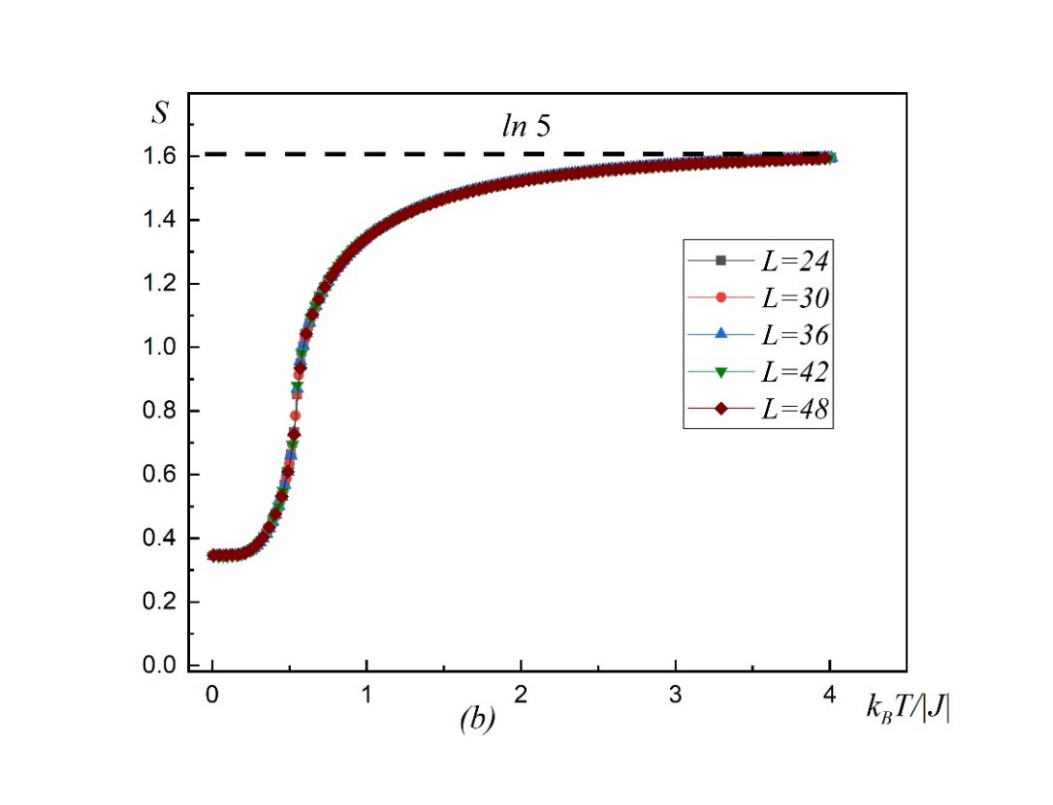
\includegraphics[width=\linewidth]{rmk/image2.jpeg}
        \caption{}
    \end{subfigure}
    \caption{Температурные зависимости энтропии S. a) для ферромагнитной модели; b) для антиферромагнитной модели.}
    \label{fig:rmk-1}
\end{figure}

Из рисунков видно, что с увеличением температуры энтропия для всех систем стремится к теоретически предсказанному значению $\ln 5$. При низких температурах, близких к абсолютному нулю, для ферромагнитной модели энтропия стремится к нулевому значению для всех значений $L$. Нулевая остаточная энтропия свидетельствует об отсутствии вырождения основного состояния. Для антиферромагнитной модели энтропия при низких температурах стремится к ненулевому значению для всех значений $L$. Такое поведение свидетельствует о сильном вырождении данной модели, что характерно для фрустрированных систем.

\begin{figure}[ht]
    \begin{subfigure}{0.5\textwidth}
        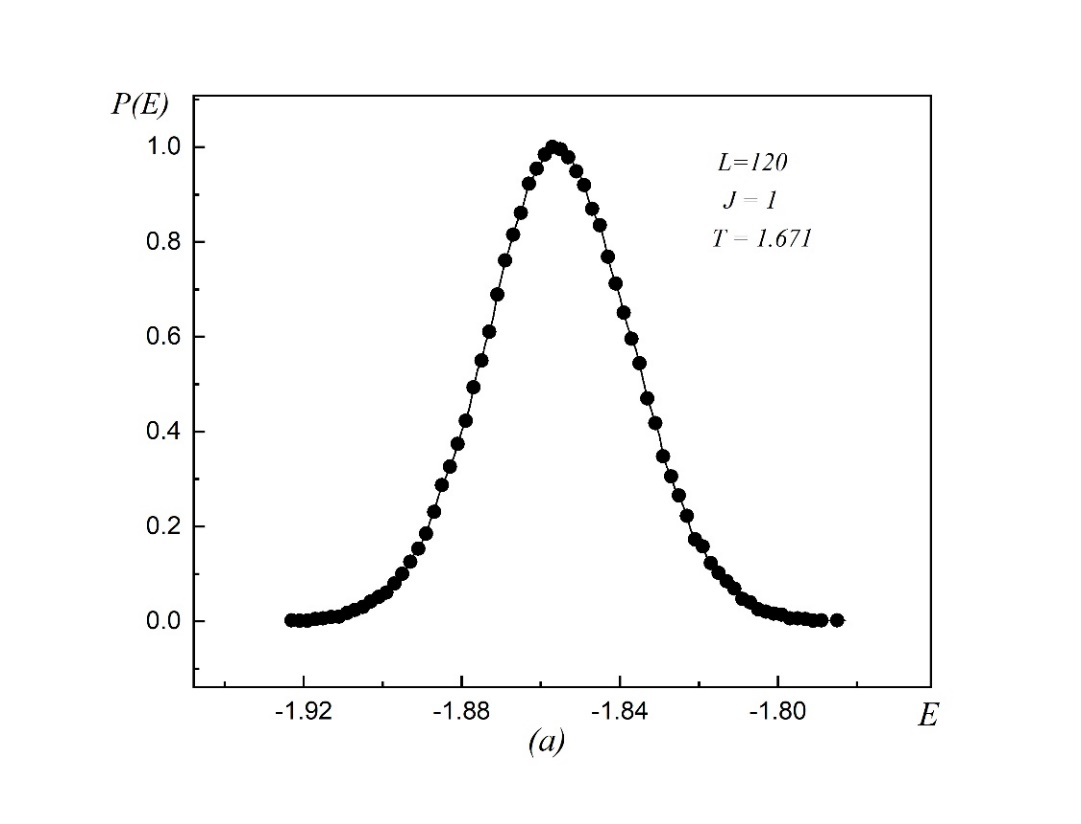
\includegraphics[width=\linewidth]{rmk/image3.jpeg}
        \caption{}
        \label{fig:rmk-2:a}
    \end{subfigure}
    \begin{subfigure}{0.5\textwidth}
        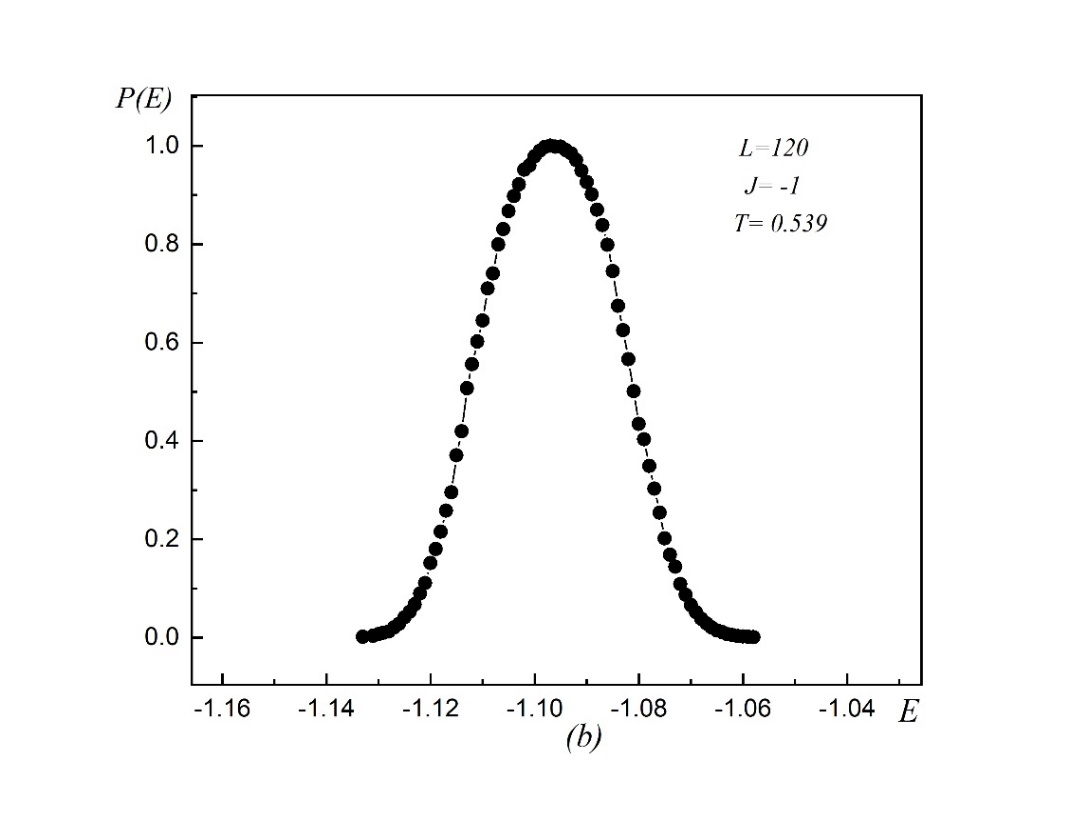
\includegraphics[width=\linewidth]{rmk/image4.jpeg}
        \caption{}
        \label{fig:rmk-2:b}
    \end{subfigure}
    \caption{Гистограмма распределения энергии. a) для ферромагнитной модели; b) для антиферромагнитной модели.}
    \label{fig:rmk-2}
\end{figure}

Для определения рода ФП мы использовали гистограммный анализ данных метода Монте-Карло. В случае ФП первого рода на гистограмме распределения энергии вблизи температуры перехода наблюдается бимодальное распределение энергии. То есть, на графике появляются два максимума, расположенных симметрично относительно равновесного значения энергии. В случае ФП второго рода должен наблюдаться один максимум. На рис.~\ref{fig:rmk-2:a} и \ref{fig:rmk-2:b} представлены гистограммы распределения энергии для линейных размеров системы $L=120$ в области температуры ФП для ферромагнитной и антиферромагнитной моделей. На графиках зависимости вероятности $P$ от энергии системы $E$ наблюдается один хорошо выраженный максимум, который свидетельствует о наличии в антиферромагнитной модели ФП второго рода. Для ферромагнитной часовой модели подобный анализ показывает наличие одного максимума, который позволяет нам утверждать, что в данной модели точно не наблюдается ФП первого рода. Такое поведение характерно для ФП второго рода.

\section*{Заключение}

Проведено исследование фазовых переходов и термодинамических свойств двумерной часовой модели на треугольной решетке с числом состояний спина $q = 5$ с использованием алгоритма Ванга-Ландау метода Монте-Карло. На основе гистограммного метода проведен анализ рода ФП данной модели. Обнаружено, что для ферромагнитной часовой модели происходят два фазовых перехода типа Березинского-Костерлица-Таулеса. Данные полученные для антиферромагнитной часовой модели свидетельствуют о том, что основное состояние системы сильно вырождено и в системе происходит ФП второго рода. Показано, что антиферромагнитное обменное взаимодействие ближайших соседей может повлиять на физические свойства часовой модели с $q=5$.

% \documentclass{article}
% \usepackage[utf8]{inputenc}
% \usepackage{graphicx}
% \usepackage[russian]{babel}
% \newtheorem{theorem}{Теорема}
% \author{Меджидов З.Г. }
% \usepackage{natbib}
% \begin{document}
\chapter{Отчет Меджидова~З.Г.}

Объект исследования - интегральные преобразования векторных и тензорных полей, заданных на семействах прямых и ломаных на плоскости и в трехмерном евклидовом пространстве. 

Цель работы  - получить формулы обращения лучевого и V-лучевого преобразований  векторных и тензорных полей.

Метод исследования - применение формул обращения классического преобразования Радона, использование моментов лучевых преобразований векторных и тензорных полей, интегрирование по частям в криволинейных интегралах.

Результат работы - получены новые формулы обращения интегральных преобразований векторных и тензорных полей, определенных на некоторых семействах прямых в пространстве и ломаных на плоскости. 

Область применения результатов - области науки и техники, связанные с неразрушающей реконструкцией: биомедицинская визуализация, национальная безопасность, гамма-астрономия и др. На основе точных формул обращения могут быть составлены алгоритмы численного восстановления.


\section{Введение}
Решаются задачи восстановления векторных и тензорных полей в трехмерном пространстве и на плоскости по заданным интегральным преобразованиям двух типов. Первое преобразование можно охарактеризовать как множество интегралов от тензорных полей, взятых по лучам, касающимся данной поверхности. Это одно из трех преобразований на трехмерных комплексах лучей, перечисленных в работе \cite{Medzhidov}. Приведенная здесь теорема обобщает теорему, доказанную в этой работе на случай тензорных полей.

Второе преобразование, называемое еще V-лучевым преобразованием, задано на семействах ломаных на плоскости. Идею V-образных преобразований Радона с фиксированным направлением оси симметрии выдвинули Трунг Т. и Нгуен М. К. (\cite{Truong}). Такие преобразования могут представлять теоретический интерес в интегральной геометрии. Они возникают в результате связанного томографического процесса пропускания-отражения. Интегральные преобразования по преломленным лучам изучаются и во многих других работах. Из недавних работ можно отметить статьи \cite{Sharafutdinov}, \cite{Ambartsoumian}  и др.
Мы рассматриваем обобщения указанных преобразований на векторные и тензорные поля на плоскости.
\section{Обращение тензорных полей по интегральным данным на семействе лучей, касающихся поверхности}
1. Пусть $f=\left(f_1, f_2 f_3\right)$ - гладкое (класса $C^2$) векторное поле с компактным носителем в трехмерном евклидовом пространстве $\mathbb R^3$, $\theta$ -единичный вектор, $x\in \mathbb R^3$,  $l=\{x+t\theta, t\geq 0\}$ - ориентированная прямая Лучевым преобразованием поля $f$ называется функция
$$If(l)=If(x,\theta)=\int_0^{+\infty}f_k(x+t\theta)\theta^kdt;$$
по повторяющемуся индексу производится суммирование от 1 до 3.

В следующей теореме, доказанной в работе \cite{Medzhidov}, решается задача реконструкции поля  $f$ по данным интегралам   на трехмерном многообразии (комплексе) прямых в  $\mathbb R^3$, касательных данной поверхности $R$. Однозначно можно восстановить только соленоидальную часть поля, что  равносильно нахождению оператора Сен-Венана $Wf$.

\begin{theorem} Пусть $R$ – гладкая поверхность в ориентированном евклидовом пространстве $\mathbb R^3$, $H$ – плоскость, трансверсальная $\Sigma$. Предположим, что кривая $C=R\cap H$ имеет гладкую (класса  ) натуральную параметризацию $y=y(s), s\in [0,S],  |y'(s)|=1$, и кривизну, отличную от нуля в каждой точке $y(s)$. Тогда для любого поля $f$, такого, что  
$supp f\cap H$ содержится в области значений отображения $[0,S]\times [0;+\infty)\to H$, поле $Wf$ может быть восстановлена по заданному полю $If(y(s), y'(s))$ и его первым производным для лучей $l=l((y(s), y'(s))$, где $s\in C$.\
\end{theorem}

Для решения аналогичной задачи для тензорных полей второго ранга мы используем доополнительные интегральные данные. 

Пусть $f$ - гладкое (класса $C^2$) симметричное тензорное поле с компактным носителем в трехмерном евклидовом пространстве $\mathbb R^3$. Его лучевое преобразование и момент первого порядка определяются соответствеенно формулами

$$If(x,\theta)=\int_0^{+\infty}f_{kl}(x+t\theta)\theta^k\theta^ldt;$$
$$I^1f(x,\theta)=\int_0^{+\infty}f_{kl}(x+t\theta)\theta^k\theta^l tdt.$$

\begin{theorem} Пусть $R, H, C$ те же, что в теореме 1. Тогда для любого поля $f$, такого, что  
$supp f\cap H$ содержится в области значений отображения $[0,S]\times [0;+\infty)\to H$, поле $Wf$ может быть восстановлена по заданным полям $If(y(s), y'(s)),  I^1f(y(s), y'(s))$ и их первым производным для лучей $l=l((y(s), y'(s))$, где $s\in C$.
\end{theorem}

\section{Обращение векторных полей по интегральным данным на семействах ломаных на плоскости} 

Пусть $ \omega=(\omega_1,\omega_2 ), \, \theta=(\theta_1,\theta_2) $  – линейно независимые единичные векторы на плоскости, $x=(x_1,x_2 )\in \mathbb R^2$ – произвольная точка. Символом $\Gamma_{\omega,\theta}(x) $ обозначим объединение двух лучей с вершиной в точке x и направляющими векторами ω и θ соответственно:
$\Gamma_{\omega,\theta}(x)= \Gamma_{\omega}(x)\cup \Gamma_\theta^-(x), \,   \Gamma_{\omega}(x)={\xi=(\xi_1, \xi_2)\in\mathbb R^2: \xi=x+\omega t, t\geq 0}
$; знак «–» в обозначении $\Gamma_\theta^-(x)$ означает, что луч $\Gamma_\theta(x)$ проходится в направлении, противоположном направлению вектора θ.

Лучевым преобразованием функции $h(x)$ называется функция

$$Xh(x;\omega)=\int_{\Gamma_\omega (x)} h(y)ds=\int_0^\infty h(x+t\omega)dt.$$
V-преобразованием Радона функции $h$ называется функция

$$Vh(x;\omega,\theta)=Xh(x;\omega)-Xh(x;\theta)=\int_{\Gamma_{\omega,\theta}(x)} h(y)ds.$$

Пусть $f=(f_1,f_2 )$ – векторное поле на плоскости. $V$-лучевым преобразованием поля $f$ называется функция

$$If(x;\omega,\theta)=X(f\cdot\omega)(x;\omega)-X(f\cdot\theta)(x;\theta),$$
где $f\cdot\omega=f_1 \omega_1+f_2 \omega_2$ – скалярное произведение. Здесь и далее предполагается, что компоненты $f_1$ и $f_2$ векторного поля принадлежат классу $C_0^2 (\mathbb R^2 )$ дважды непрерывно дифференцируемых финитных функций.


Задача состоит в том, чтобы по заданному преобразованию $If$ определить неизвестное поле $f$. Однозначно определить поле $f$ по заданной функции $If$ невозможно, так как $I(\nabla h)=0$, где 

$$\nabla h=\left(\frac{\partial h}{\partial x_1},\frac{\partial h}{\partial x_2}\right),$$
т.е. $f$ можно найти с точностью до потенциального слагаемого. Требуются дополнительные интегральные данные.

Определим также преобразование

$$Jf(\omega,\theta)=X(f\cdot \omega)(x;\omega^\bot )-X(f\cdot\theta)(x;\theta^\bot),$$
называемое поперечным V-лучевым преобразованием поля $f$.

Пусть $\partial_\theta f=(\theta,\nabla f)$ – производная скалярного поля $f$ по направлению вектора $\theta$, 
$$\delta f=\frac{\partial f_1}{\partial x_1}+\frac{\partial f_2}{\partial x_2},\,\, \delta^\bot f=\frac{\partial f_2}{\partial x_1}-\frac{\partial f_1}{\partial x_2}$$
–дивергенция и ортогональная дивергенция поля $f$, соответственно.


\begin{theorem} Ядро оператора $I$ состоит из потенциальных векторных полей, т.е.
$$If=0 \Leftrightarrow f=\nabla h$$ 
для некоторой функции $h$.
Ядро оператора $J$ состоит из соленоидальных векторных полей, т.е.
$$Jf=0  \Leftrightarrow  \delta f=0.$$
\end{theorem}

\begin{theorem} Векторное поле $f$ однозначно восстанавливается по заданным ее V-лучевому и поперечному V-лучевому преобразованиям.
\end{theorem}

Для полного восстановления поля $f$ введем интегральные данные другого вида.
Интегральное преобразование 
$$I^1 f(x;\omega,\theta)=X^1 (f\cdot\omega)(x;\omega)-X^1 (f\cdot\theta)(x;\theta)$$
назовем моментом первого порядка V-лучевого преобразования функции поля $f$, где
$$X^1 h(x;\omega)=\int_0^\infty h(x+t\omega )tdt$$
– момент первого порядка лучевого преобразования функции $h$.

\begin{theorem} Векторное поле $f$ с компонентами из класса $C_0^2 (\mathbb R^2 )$ дважды непрерывно дифференцируемых финитных функций однозначно восстанавливается по заданным ее V-лучевому преобразованию $If$ и моменту первого порядка V-лучевого преобразования $I^1 f$.
\end{theorem}

\begin{theorem} Векторное поле $f$ однозначно восстанавливается по заданным ее поперечному V-лучевому преобразованию $Jf$ и моменту первого порядка поперечного V-лучевого преобразования $J^1 f$.
\end{theorem}




\section{Заключение}
Решены задачи обращения лучевого и V-лучевого преобразований векторных и тензорных полей на плоскости и в пространстве. Отличие данных результатов от результатов других авторов состоит в том, что восстанавливается векторное поле целиком, при этом используются моменты первого порядка, а в случае тензорного поля определяется оператор Сен-Венана.
Методы решения приведенных задач могут быть применены при обращении лучевых преобразований и V-лучевых преобразований тензорных полей высокого ранга.

Результаты п.1 планируется опубликовать в ближайшем номере ДЭМИ.
Результаты п.2 сданы в Вестник ДГУ, их обобщения на тензорные поля планируется отправить в один из центральных журналов.




% \documentclass{article}

% % Figure setup
% \usepackage{graphicx}
% \graphicspath{{./images/}}
% \usepackage{subcaption}

% % Ref setup
% \usepackage{hyperref}

% % Cite setup
% \usepackage{cite}

% % Font setup
% \usepackage{fontspec}
% \setmainfont{Times New Roman}

% % Lang setup
% \usepackage{polyglossia}
% \setdefaultlanguage{russian}
% \setotherlanguage{english}

% \renewcommand{\UrlFont}{\ttfamilylatin}

\chapter{Исследование фазовых переходов, магнитных, термодинамических и критических свойств в магнитных спиновых системах}
% \author{Магомедов Магомед Алиевич}
% \date{}

% \begin{document}

% \maketitle

%% \begin{abstract}
%    Методом Ванга-Ландау исследована векторная пятихвершинная модель Поттса на треугольной решетке с учетом конкурирующего обменного взаимодействия между первыми и вторыми ближайшими соседями. Вычислена плотность состояний системы $g(E)$, определены магнитные структуры основного состояния и рассчитаны температурные зависимости различных термодинамических параметров, таких как внутренняя энергия $E$, теплоемкость $C$, энтропия $S$. Показано, что в зависимости от знака обменного взаимодействия между спинами, основное состояние может быть ферромагнитным либо сильно вырожденным.
%% \end{abstract}
%
%\textbf{Целью настоящей работы} является исследование векторной модели Поттса с числом состояний $q=5$ на треугольной решетке методами вычислительной физики.
%
%\textbf{Объектом исследования} являлась векторная модель Поттса с числом состояний $q=5$ на треугольной решетке.
%
%\textbf{Методы исследования.} Для исследования векторной модели Поттса с числом состояний $q=5$ на треугольной решетке нами был разработан комплекс программ для ЭВМ, основанный на алгоритме Ванга-Ландау. Методика исследований, предложенная нами, позволяет не только рассчитать температурные зависимости различных термодинамических параметров, но также определить структуру основного состояния системы, выявить наличие фрустрации или вырождения основного состояния, а также рассчитать энтропию и свободную энергию, что невозможно при использовании других методов. Важной особенностью реализованного нами метода является возможность снятия <<снимка>> основного состояния -- сохранения в графическом файле структуры основного состояния, которая позволяет рассмотреть, какое упорядочение реализуется в системе вблизи абсолютного нуля.

\section{Введение}

Исследование фазовых переходов (ФП), магнитных, термодинамических и критических свойств в магнитных спиновых системах представляет большой теоретический и экспериментальный интерес. Это связано с тем, что для большинства реальных магнитных спиновых систем характерны возмущения различной природы, такие как анизотропия, взаимодействия следующих за ближайшими соседей, внешнее магнитное поле, тепловые и квантовые флуктуации, немагнитные примеси, дефекты, деформации и др. Присутствие этих факторов может повлиять на природу ФП и термодинамические характеристики таких систем \cite{bib:mma-1,bib:mma-2,bib:mma-3,bib:mma-4,bib:mma-5,bib:mma-6,bib:mma-7,bib:mma-8,bib:mma-9,bib:mma-10,bib:mma-11}. Для изучения особенностей термодинамического поведения и природы ФП успешно используются различные решеточные модели. На их основе получено большое количество интересных результатов. Решеточные спиновые модели позволяют описать целый ряд реальных магнитных материалов.

Одной из моделей, применяемых для описания физических систем, является векторная модель Поттса с числом состояний спина $q$. Нами в данном исследовании рассматривается векторная модель Поттса с числом состояний спина $q=5$ на треугольной решетке. Магнитные материалы на треугольной решетке представляют особый интерес для исследователей. Антиферромагнетики на треугольной решетке представляют собой геометрически фрустрированные спиновые системы, которые исследуются уже давно. Для фрустрированных систем существует совсем немного надежно установленных фактов. Большинство имеющихся результатов получены для модели Изинга, Гейзенберга и Поттса с числом состояний спина $q = 2$, $3$ и $4$.

Многие физические свойства часовой модели зависят от значения $q$. В случае, когда $q = 2$, $3$, $4$, эта модель имеет точное решение. Векторная модель Поттса сводится к модели Изинга и $Z_3$ модели Поттса при $q = 2$ и $3$, соответственно. При $q = 4$ данная модель эквивалентна двум копиям модели Изинга. Установлено, что для этих трех случаев в системе наблюдается ФП второго рода из высокотемпературной парамагнитной фазы в низкотемпературную ферромагнитную упорядоченную фазу. Когда $q \to \infty$ данная векторная модель Поттса сводится к стандартной $XY$ модели. В этом случае спонтанного нарушения симметрии не наблюдается, но происходит ФП из низкотемпературной фазы Березинского-Костерлица-Таулеса (БКТ) в высокотемпературную парамагнитную фазу. Для часовой модели с числом состояний спина $q = 5$ имеется очень мало точно установленных фактов. К настоящему моменту остается открытым вопрос о роде ФП при значении $q = 5$.

Для получения ответа на этот вопрос в данной работе нами проводится исследование двумерной векторной модели Поттса на треугольной решетке с $q = 5$. Исследование этой модели с антиферромагнитными обменными взаимодействиями на треугольной решетке в литературе практически не встречается. Антиферромагнитное обменного взаимодействие в данной модели может привести к фрустрации, вырождению основного состояния, появлению различных фаз и ФП, а также влиять на его термодинамические, магнитные и критические свойства. В связи с этим в данной работе нами предпринята попытка провести исследование ФП и термодинамических свойств этой модели на треугольной решетке.

Исследования проводятся на основе современных методов и идей, что позволит получить ответ на ряд вопросов, связанных с природой ФП и термодинамическим поведением фрустрированных спиновых систем.

\section{Векторная модель Поттса с \texorpdfstring{$q=5$}{q=5} на треугольной решетке}

Далее нами приводятся результаты исследования векторной модели Поттса на треугольной решетке методом Ванга-Ландау \cite{bib:mma-9,bib:mma-10,bib:mma-11}. Модель Поттса была предложена в 1952 году Поттсом по предложению С. Домба. Модель задается числом состояний $q$, в которых может находиться спин на произвольной решетке.

Гамильтониан векторной модели Поттса с числом состояний $q=5$ на треугольной решетке может быть представлен в следующем виде:
\begin{equation}
    \label{eq:mma-1}
    H = -J \sum_{i, j} \cos \left(\theta_i - \theta_J\right),
\end{equation}
где спиновые состояния $q$ в узле $i$ обозначены плоским углом $\theta_i = 2\pi k/q$, $k = 1, \dots, q$. В данном исследовании нами рассматриваются два случая. В первом случае $J > 0$ -- параметр ферромагнитного обменного взаимодействия, а во втором случае $J < 0$ -- параметр антиферромагнитного обменного взаимодействия.

Схематическое и цветовое представление модели представлено на рисунке \ref{fig:mma-1}. На вставке приведены направления спинов для каждого из 5 значений спина и соответствующее цветовое представление. Как видно из рисунка, каждый спин взаимодействует с шестью своими ближайшими соседями.
\begin{figure}[ht]
    \centering
    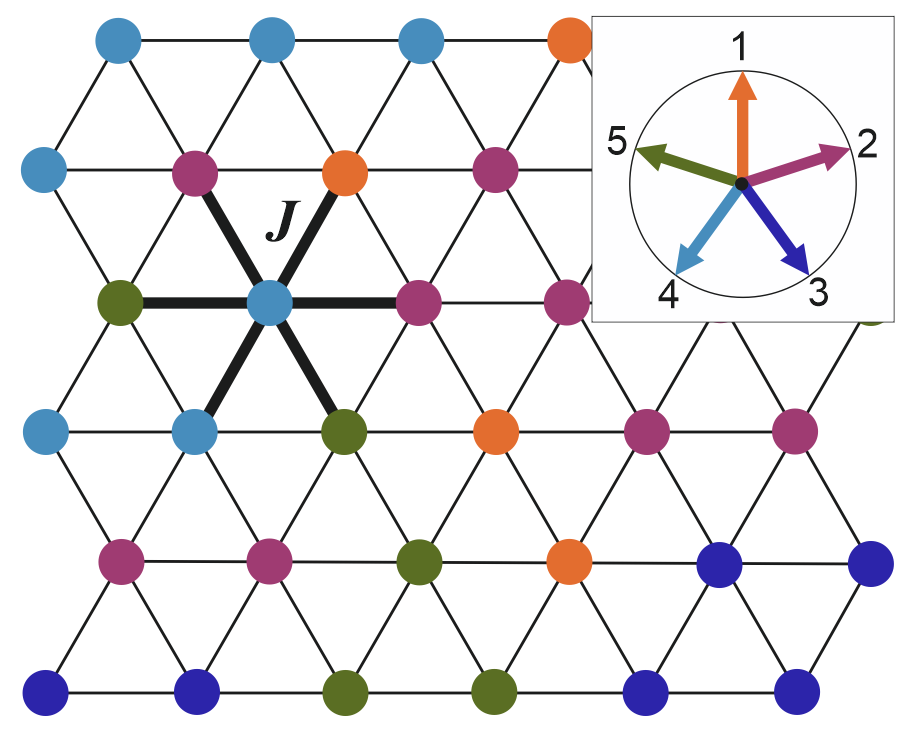
\includegraphics[width=0.8\textwidth]{mma/image2.png}
    \caption{Векторная модель Поттса с числом состояний спина $q = 5$ на треугольной решетке.}
    \label{fig:mma-1}
\end{figure}

\section{Метод исследований}

Исследования проводились на основе алгоритма Ванга-Ландау метода Монте-Карло (МК) \cite{bib:mma-9,bib:mma-10,bib:mma-11}. Данный алгоритм является реализацией метода энтропийного моделирования и его основной особенностью является возможность расчета функции плотности состояний системы, зная которую можно легко вычислить любые интересующие нас термодинамические параметры системы.

Алгоритм Ванга-Ландау является разновидностью энтропийного моделирования и, как показывает опыт его применения в последние годы, является весьма эффективным для исследования различных дискретных спиновых систем \cite{bib:mma-9}.

Алгоритм Ванга-Ландау основан на том, что совершая случайное блуждание в пространстве энергий с вероятностями, обратно пропорциональными плотности состояний $g(E)$, мы получаем равномерное распределение по энергиям. Подобрав вероятности перехода такими, что посещение всех энергетических состояний стало бы равномерным, можно получить изначально неизвестную плотность состояний $g(E)$, зная которую можно вычислить значения необходимых термодинамических параметров при любой температуре. Так как плотность состояний $g(E)$ очень быстро растет с увеличением размеров исследуемых систем, для удобства хранения и обработки больших чисел пользуются величиной $\ln g(E)$.

Важным обстоятельством является то, что плотность состояний $g(E)$ не зависит от температуры, следовательно, рассчитав ее однократно, мы можем вычислить значения любых термодинамических параметров системы при любой ненулевой температуре.

В данной работе нами алгоритм Ванга-Ландау был использован в следующем виде \cite{bib:mma-9,bib:mma-10,bib:mma-11}:
\begin{itemize}
    \item Задается произвольная начальная конфигурация спинов. Стартовые значения плотности состояний $g(E)=1$, гистограммы распределений по энергиям $H(E)=1$ и начальное значение модификационного фактора $f = f_0 = e^1 \approx 2.71828$.
    \item Многократно совершаем шаги в фазовом пространстве, пока не получим относительно плоскую гистограмму $H(E)$ (т.е. пока не будут посещены примерно одинаковое количество раз все возможные энергетические состояния системы). В качестве критерия <<плоскости>> гистограммы нами принималось условие отклонения числа посещений всех возможных (с ненулевой плотностью $g(E) \neq 1$) энергетических состояний на величину не более чем на 10\% от среднего значения по системе.
    \item При этом вероятность перехода из состояния с энергией $E_1$ в состояние с энергией $E_2$ определяется по формуле $p = g(E_1) / g(E_2)$. Если переход в состояние с энергией $E_2$ состоялся, то для энергии $E_2$ проводится модификация плотности состояния $g(E_2) \to f \times g(E_2)$, и гистограммы $H(E_2) \to H(E_2) + 1$ иначе меняем параметры для энергии $E_1$ $g(E_1) \to f \times g(E_1)$ $H(E_1) \to H(E_1) + 1$.
    \item Если гистограмма стала <<плоской>>" то: обнуляем гистограмму $H(E) \to 0$,  уменьшаем модификационный фактор $f \to \sqrt{f}$, и продолжаем снова и снова, пока модификационный фактор $f \geq f_{\min}$. В качестве минимального значения модификационного фактора нами принималось $f_{\min} = 1.0000000001$.
    \item Каждый раз при достижении энергетического минимума нами проводился анализ магнитной структуры основного состояния и его запись в графический файл. При этом проводилось сравнение полученной конфигурации с ранее полученными и только при обнаружении новой уникальной конфигурации производится ее сохранение в графический файл. Далее данная структура заносится в специальную базу данных для данной модели для дальнейшего сравнения. Данная процедура позволяет избежать дублирования в графических файлах многократно встречающихся состояний с одинаковой магнитной структурой.
    \item После расчета плотности состояний системы для любой интересующей нас температуры рассчитываются различные термодинамические параметры, такие как, энтропия, внутренняя энергия, свободная энергия, теплоемкость, намагниченность, восприимчивость и т.д.
\end{itemize}

Более подробно алгоритм Ванга-Ландау изложен в работах \cite{bib:mma-9,bib:mma-10,bib:mma-11}.

\section{Векторная пятихвершинная модель Поттса на треугольной решетке}

На рис.~\ref{fig:mma-2} приведены плотности состояний $g(E)$ для разных линейных размеров системы для ферромагнитной и антиферромагнитной моделей (здесь и далее статистическая погрешность не превышает размеров символов, использованных для построения зависимостей). Как видно на рисунке, плотность состояний имеет куполообразную форму. С увеличением линейных размеров системы максимум плотности состояний $g(E)$ значительно возрастает.
\begin{figure}[ht]
    \begin{subfigure}{0.5\textwidth}
        \includegraphics[width=0.9\linewidth]{mma/image17.png}
        \caption{для ферромагнитной модели;}
    \end{subfigure}
    \begin{subfigure}{0.5\textwidth}
        \includegraphics[width=0.9\linewidth]{mma/image18.png}
        \caption{для антиферромагнитной модели;}
    \end{subfigure}
    \caption{Плотность состояний $g(E)$ при различных линейных размерах $L$.}
    \label{fig:mma-2}
\end{figure}

На рис.~\ref{fig:mma-3}. представлены характерные зависимости теплоемкости $C$ от температуры для ферромагнитной и антиферромагнитной моделей с различными линейными размерами системы $L$. Отметим, что для ферромагнитной модели (рис.~\ref{fig:mma-3a}) на зависимостях теплоемкости $C$ от температуры для всех систем вблизи критической температуры наблюдаются два хорошо выраженных максимума. Наличие двух максимумов на температурной зависимости теплоемкости позволяет говорить о двух последовательных ФП в данной модели.
\begin{figure}[ht]
    \begin{subfigure}{0.5\textwidth}
        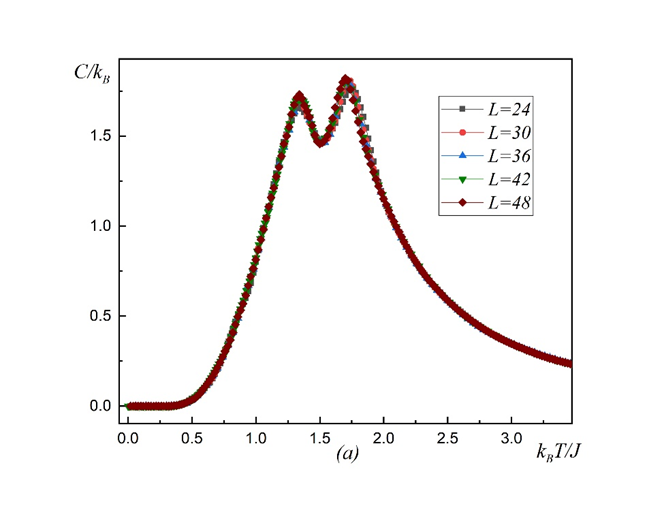
\includegraphics[width=0.9\linewidth]{mma/image19.png}
        \caption{для ферромагнитной модели;}
        \label{fig:mma-3a}
    \end{subfigure}
    \begin{subfigure}{0.5\textwidth}
        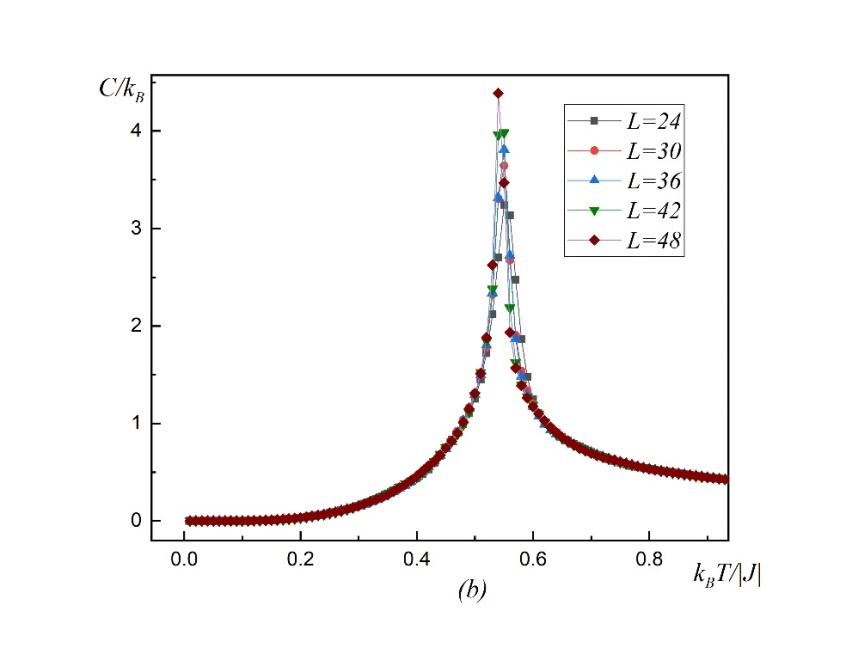
\includegraphics[width=0.9\linewidth]{mma/image20.jpeg}
        \caption{для антиферромагнитной модели;}
        \label{fig:mma-3b}
    \end{subfigure}
    \caption{Зависимость теплоемкости $C/k_B$ от температуры $k_B T/ \left|J\right|$ для разных $L$.}
    \label{fig:mma-3}
\end{figure}

\begin{figure}[ht]
    \begin{subfigure}{0.33\textwidth}
        
\includegraphics[width=0.9\linewidth]{mma/image21.png}
        \caption{в интервале температур $0 \leq T < Tc_1$;}
        \label{fig:mma-4a}
    \end{subfigure}
    \begin{subfigure}{0.33\textwidth}
        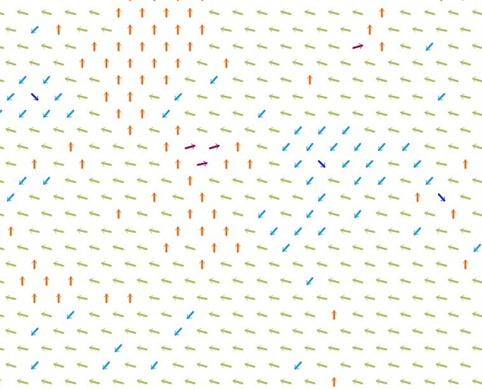
\includegraphics[width=0.9\linewidth]{mma/image22.png}
        \caption{в интервале температур $Tc_1 < T < Tc_2$;}
        \label{fig:mma-4b}
    \end{subfigure}
    \begin{subfigure}{0.33\textwidth}
        
\includegraphics[width=0.9\linewidth]{mma/image23.png}
        \caption{$T > Tc_2$;}
        \label{fig:mma-4c}
    \end{subfigure}
    \caption{Магнитные структуры основного состояния для ферромагнитной модели;}
    \label{fig:mma-4}
\end{figure}

Для антиферромагнитной модели (рис.~\ref{fig:mma-3b}) наблюдается только один максимум, что позволяет говорить об одном ФП. Все максимумы увеличиваются с ростом числа спинов в системе, причем они в пределах погрешности приходятся на одну и ту же температуру даже для систем с наименьшим значением $L$. Это свидетельствует, во-первых, о высокой эффективности использованного способа добавления периодических граничных условий, а во-вторых, о достижении насыщения по $N$ для многих исследуемых нами параметров.

Для определения типа упорядочения нами проведен анализ магнитных структур основного состояния в широком температурном интервале. На рис.~\ref{fig:mma-4} приведены полученные нами структуры. На рисунке видно, что в данной модели наблюдаются три типа магнитного упорядочения: в интервале температур $0 \leq T < Tc_1$ (рис.~\ref{fig:mma-4a}) наблюдается полностью упорядоченная ферромагнитная фаза; в интервале $Tc_1 < T < Tc_2$ (рис.~\ref{fig:mma-4b}) -- фаза типа Березинского-Костерлица-Таулеса, где наблюдается ближний порядок в системе, в котором превалирует одно из пяти состояний спина; при дальнейшем повышении температуры $T > Tc2$ (рис.~\ref{fig:mma-4c}) -- полностью разупорядоченная парамагнитная фаза.

\begin{figure}[ht]
    \begin{subfigure}{0.5\textwidth}
        \includegraphics[width=0.9\linewidth]{mma/image24.png}
        \caption{для ферромагнитной модели;}
    \end{subfigure}
    \begin{subfigure}{0.5\textwidth}
        \includegraphics[width=0.9\linewidth]{mma/image25.png}
        \caption{для антиферромагнитной модели;}
    \end{subfigure}
    \caption{Температурные зависимости энтропии $S$.}
    \label{fig:mma-5}
\end{figure}

На рис.~\ref{fig:mma-5} приведены температурные зависимости энтропии $S$ для обоих моделей. Из рисунков видно, что с увеличением температуры энтропия для всех систем стремится к теоретически предсказанному значению $\ln 5$. При низких температурах, близких к абсолютному нулю, для ферромагнитной модели энтропия стремится к нулевому значению для всех значений $L$. Нулевая остаточная энтропия свидетельствует об отсутствии вырождения основного состояния. Для антиферромагнитной модели энтропия при низких температурах стремится к ненулевому значению для всех значений $L$. Такое поведение свидетельствует о сильном вырождении данной модели, что также характерно для фрустрированных систем.

Для анализа характера ФП использовался метод кумулянтов Биндера четвертого порядка по энергии, который имеет следующий вид:
\begin{equation}
    \label{eq:mma-2}
    V_L (T) = 1 - \frac{\left<E^4\right>}{\left<E^2\right>^2}
\end{equation}

Известно, что ФП второго рода характеризуются следующими отличительными особенностями: усредненная величина $V_L (T)$ стремится к тривиальному значению согласно выражению $V_L (T) = V* + b L^{-d}$ при $L \to \infty$ и $T = T(L)$, где $V* = 2/3$.

Характерные зависимости кумулянтов Биндера $V_L(T)$ от температуры для систем с линейными размерами для ферромагнтной и антиферромагнитной моделей приведены на рис.~\ref{fig:mma-6}. Как видим из рисунков энергетические кумулянты для обоих моделей показывают разный характер поведения. Для антиферромагнитного случая на графиках зависимости энергетических кумулянтов наблюдаются минимумы в области температуры фазового перехода, которые уменьшаются с увеличением размеров системы $L$. Для ферромагнитной модели такие минимумы не наблюдаются. Заметим, что на вставке к рис.~\ref{fig:mma-6b} наглядно видно, что тривиальная величина $V* \to 2/3$ при $L \to \infty$. Такое поведение, как отмечалось выше, характерно для ФП второго рода.
\begin{figure}[ht]
    \begin{subfigure}{0.5\textwidth}
        \includegraphics[width=0.9\linewidth]{mma/image27.png}
        \caption{для ферромагнитной модели;}
        \label{fig:mma-6a}
    \end{subfigure}
    \begin{subfigure}{0.5\textwidth}
        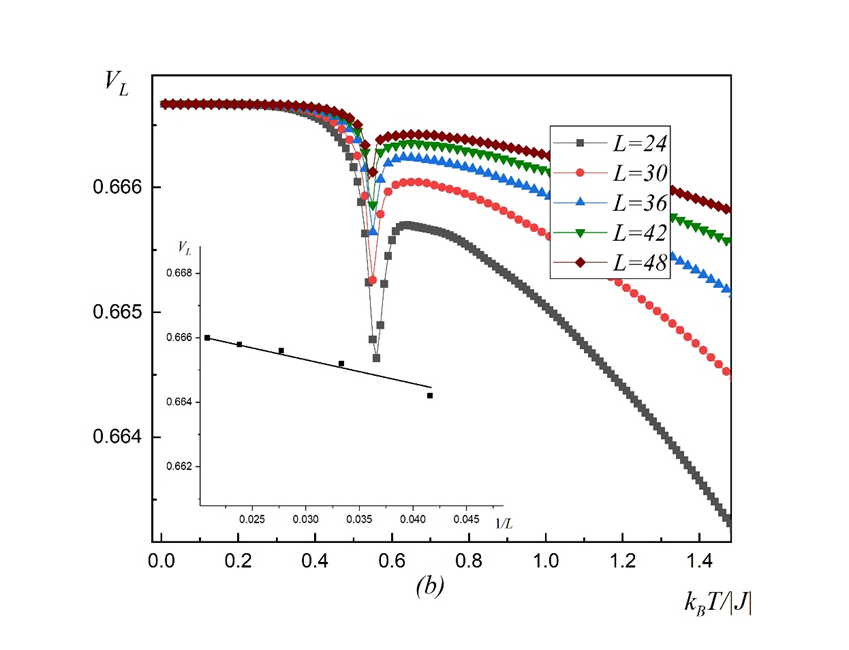
\includegraphics[width=0.9\linewidth]{mma/image28.png}
        \caption{для антиферромагнитной модели;}
        \label{fig:mma-6b}
    \end{subfigure}
    \caption{Температурная зависимость кумулянтов Биндера $V_L (T)$.}
    \label{fig:mma-6}
\end{figure}

Для более точного определения рода ФП мы использовали гистограммный анализ данных метода МК. В случае ФП первого рода на гистограмме распределения энергии вблизи температуры перехода наблюдается бимодальное распределение энергии. То есть, на графике появляются два максимума, расположенных симметрично относительно равновесного значения энергии. В случае ФП второго рода должен наблюдаться один максимум.

\begin{figure}[ht]
    \begin{subfigure}{0.5\textwidth}
        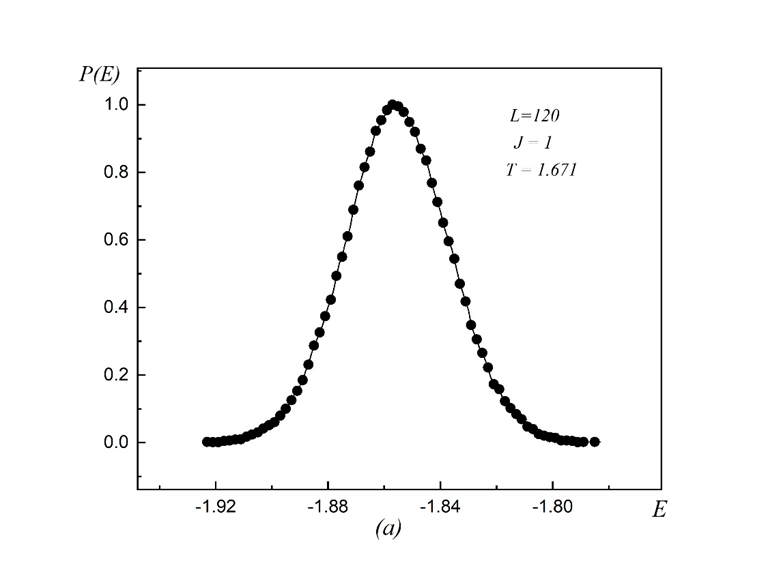
\includegraphics[width=0.9\linewidth]{mma/image29.png}
        \caption{для ферромагнитной модели;}
        \label{fig:mma-7a}
    \end{subfigure}
    \begin{subfigure}{0.5\textwidth}
        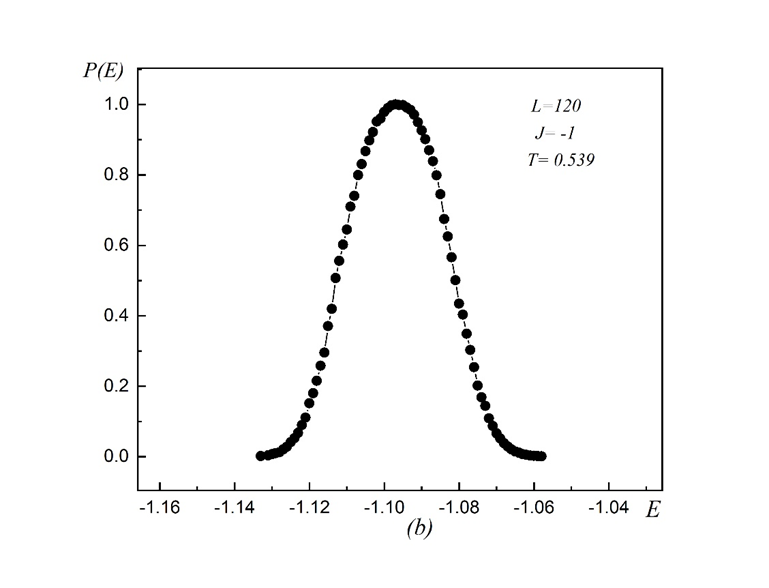
\includegraphics[width=0.9\linewidth]{mma/image30.png}
        \caption{для антиферромагнитной модели;}
        \label{fig:mma-7b}
    \end{subfigure}
    \caption{Гистограмма распределения энергии.}
    \label{fig:mma-7}
\end{figure}

На рис.~\ref{fig:mma-7a} и \ref{fig:mma-7b} представлены гистограммы распределения энергии для линейных размеров системы $L =120$ в области температуры ФП для ферромагнитной и антиферромагнитной моделей. На графиках зависимости вероятности $P$ от энергии системы $E$ наблюдается один хорошо выраженный максимум, который свидетельствует о наличии в антиферромагнитной модели ФП второго рода. Для ферромагнитной часовой модели подобный анализ показывает наличие одного максимума, который позволяет нам утверждать, что в данной модели точно не наблюдается ФП первого рода. Такое поведение характерно для ФП второго рода. Однако, анализ магнитных структур основного состояния свидетельствует в пользу перехода типа Березинского-Костерлица-Таулеса (рис.~\ref{fig:mma-4}).

%\section*{Заключение}
%
%Выполнено исследование магнитных структур основного состояния, фазовых переходов и термодинамических свойств двумерной векторной модели Поттса с числом состояний спина $q=5$ на треугольной решетке. В работе использован алгоритм Ванга-Ландау энтропийного метода Монте-Карло. Получены магнитные структуры основного состояния. Анализ полученных данных показывает, что для ферромагнитной модели на температурной зависимости теплоемкости наблюдаются два максимума. На основе метода кумулянтов Биндера и гистограммного метода проведен анализ рода ФП данной модели. Обнаружено, что для ферромагнитной модели происходят два фазовых перехода типа Березинского-Костерлица-Таулеса. Данные полученные для антиферромагнитной часовой модели свидетельствуют о том, что основное состояние системы сильно вырождено и в системе происходит ФП второго рода. Показано, что антиферромагнитное обменное взаимодействие ближайших соседей может повлиять на физические свойства векторной модели Поттса с числом состояний $q=5$.
%
%Таким образом, по проделанной работе можно сделать следующие выводы:
%\begin{itemize}
%    \item Предложена векторная модель Поттса с числом состояний $q=5$ на треугольной решетке;
%    \item Разработана программа для ЭВМ, основанная на новейшем алгоритме Ванга-Ландау, позволяющая исследовать векторную модель Поттса с числом состояний $q=5$ на треугольной решетке;
%    \item Методом Ванга-Ландау вычислены плотности состояний $g(E)$ для векторной модели Поттса с числом состояний $q=5$ на треугольной решетке.
%    \item Определены магнитные структуры основного состояния;
%    \item Рассчитаны температурные зависимости различных термодинамических параметров, таких как свободная энергия $F$, внутренняя энергия $E$, энтропия $S$, теплоемкость  $C$;
%    \item Показано, что энтропия для данной модели при температурах близких к абсолютному нулю для ферромагнитного случая стремится к нулю, а для антиферромагнитного случая стремится к $S_0=0.333$, которое соответствует сильно вырожденному состоянию. С повышением температуры энтропия во всех случаях стремится к теоретически предсказанному значению $\ln 5$;
%\end{itemize}
%
%Результаты, полученные в ходе исследований, могут быть полезными для описания различных низкоразмерных магнитных материалов, имеющих треугольную структуру.

%\section*{Публикации}
%
%\begin{enumerate}
%    \item Муртазаев А.К., Бадиев М.К., Магомедов М.А., Рамазанов М.К. Термодинамическое поведение двумерной часовой модели с числом состояний спина q = 5 // ФТТ. 2023. Т.65. вып. 8. С. 1399 -- 1402.  DOI: 10.21883/FTT.2023.08.56161.78.
%    \item Бабаев А.Б., Муртазаев А.К. Моделирование трехкомпонентной модели Поттса на гексагональной решетке методом Монте-Карло // Физика металлов и металловедение. 2023. Т.124. № 7. С. 577--583. Babaev A.B., Murtazaev A.K. Simulation of the three-component Potts model on a hexagonal lattice by the Monte Carlo method // Physics of Metals and Metallography, vol. 124, No. 7, pp. 221--225 (2023) Published: 26 May 2023 DOI:10.31857/S0015323023600454
%\end{enumerate}
%
%\textbf{Публикации в трудах международных и российских конференций:}
%\begin{enumerate}
%    \item Бадиев М.К., Муртазаев А.К., Магомедов М.А., Рамазанов М.К. Критическое поведение часовой модели с числом состояний спина q = 5 на треугольной решетке // Сборник трудов международной конференции «Фазовые переходы, критические и нелинейные явления в конденсированных средах». Махачкала, 10-15 сентября 2023г., С.50-52. \url{https://www.dagphys.ru/upload/files/conference/2023_Conference.pdf}
%\end{enumerate} 

\backmatter

\Conclusion{content/conclusion.tex}

\begin{thebibliography}{111}

  % Ниже указаны примеры форматирования литературы
\bibitem{Ram-Ba-Ra-Pe}
{Barry P. Rajkovi\'c P.M., Petkovi\'c M.D.}
An application of Sobolev orthogonal polynomials to the computation of a special Hankel determinant
//
In book: Approximation and Computation (Chapter 4).
--- 2011.
--- Vol. 42.
--- P. 53---60.

\bibitem{Ram-Mar-Xu}
{Marcell\'an F., Xu Y.}
On Sobolev orthogonal polynomials
//
Expo Math.
--- 2015.
--- Vol. 33.
--- P. 308---352.

\bibitem{mmg-SharapudinovUMN}
Шарапудинов И.И.
Ортогональные по Соболеву системы функций и некоторые их приложения
//
УМН
--- 74:4(448)
--- 2019.
--- С. 87---164.

\bibitem{tad-SHII-Haar}
Шарапудинов И.И.
О базисности системы Хаара в пространстве $L^{p(t)}([0,1])$ и принципе локализации в среднем
//
Мат. сборник.
--- 1986.
--- Т. 130(172), № 2(6).
--- С. 275---283.
\bibitem{tad-SHII-AnalisysMath}
Sharapudinov I.I. Some aspects of approximation theory in the spaces $L^{p(x)}(E)$
//
Analysis Mathematica.
--- 2007.
--- Vol 33.
--- P. 135---153.
\bibitem{tad-SHII-Leg} О базисности системы полиномов Лежандра в пространстве Лебега $L^{p(x)}(-1,1)$ с переменным показателем $p(x)$ // Мат. сборник. --- 2009. --- Том 200, № 1. --- С. 137---160.
\bibitem{tad-MMG-Haar}
Магомед-Касумов М.Г.
Базисность системы Хаара в весовых пространствах Лебега с переменным показателем
//
Владикавк. матем. журн.
--- 2014.
--- Т. 16, № 3.
--- С. 38---46.
\bibitem{tad-SHII-Jacob}Шарапудинов И.И., Шах-Эмиров Т.Н. Сходимость рядов Фурье по полиномам Якоби в весовом пространстве Лебега с переменным показателем // Дагестанские электронные математические известия. --- 2017. --- Вып. 8. --- С. 27---47.
%\bibitem{tad-MMG-Haar} Магомед-Касумов М.Г. Базисность системы Хаара в весовых пространствах Лебега с переменным показателем // Владикавк. матем. журн. --- 2014. Том 16, № 3. --- С. 38---46.
\bibitem{tad-SHII-Ult}Шарапудинов И.И. О базисности ультрасферических полиномов Якоби в весовом пространстве Лебега с переменным показателем // Мат. заметки. --- 2019. --- Том 106, № 4. --- С. 616---638.
\bibitem{tad-RAM-Jacob} Shakh-Emirov T.N., Gadzhimirzaev R.M.  The Convergence of the Fourier–Jacobi Series in Weighted Variable Exponent Lebesgue Spaces // Operator Theory and Differential Equations. Trends in Mathematics. Birkhäuser, Cham.  In: Kusraev, A.G., Totieva, Z.D. (eds). --- 2021. --- Pp. 205---227.
    
\bibitem{bib:ark-1} Смирнов~В.И. Курс высшей математики. Т.~2.
--- М.: Наука, 1967. 

\bibitem{bib:ark-2} Кратцер~А., Франц~Ф. Трансцендентные функции.
 --- М.: Мир, 1963.

\bibitem{bib:ark-3} Никифоров~А.Ф., Уваров~В.Б. Специальные функции математической физики.
 --- М.: Наука, 1984.

\bibitem{bib:ark-4}  Бахвалов~Н.С. Численные методы.
--- М.: Наука, 1973. 

\bibitem{bib:ark-5}  Варга~Р. Функциональный анализ и теория аппроксимации
в численном анализе. --- М.: Мир, 1974. 

\bibitem{bib:ark-6} Parter~S.V. Numerical methods for generalized axially symmetric potentials
 // SIAM Journal. Series B2.  --- 1965.  --- P.~500---516.

\bibitem{bib:ark-7}  Jamet~P. On the convergence of finite-difference 
approximations to one-dimensional singular boundary-value problems
 // Numer. Math.  --- 1970. --- Vol.~14. --- P.~355---378.

\bibitem{bib:ark-8}  Natterer~F. A generalized spline method for singular boundary value problems in ordinary differential equations
 //Linear Algebra Appl. --- 1973. --- Vol.~7. --- P.~189---216.

\bibitem{bib:ark-9} Brabston~D.C., Keller~H.B. A numerical method for singular
 two point  boundary value problems
 // SIAM Journal Numer. Anal. --- 1977. --- Vol.~14. --- P.~779---791.

\bibitem{bib:ark-10}  Weinmuller~E. A difference  method for a singular
 boundary value problem of second order
 // Math. Comput. --- 1984. --- Vol.~42. --- P.~441---464. 
 
\bibitem{bib:ark-19} Рамазанов~А.-Р.К., Магомедова~В.Г. О решении начальной задачи для 
нормальной системы с помощью рациональных сплайн-функций // Вестник Дагестанского 
государственного университета. Серия~1. Естественные науки. --- 2023. --- Том~38. Вып.~1. 
--- С.~33-–39. 

% MZG

\bibitem{Medzhidov}  Меджидов З. Г. Формулы обращения тензорной томографии по неполным данным // ДЭМИ. --- 2014. Вып. 2. --- С. 75---86.
\bibitem{Truong} Truong T. T., Nguen M. K. On V-line Radon transform in $R^2$   and thear inversion // J. Phis. A: Math. Theor. --- 2011. --- Vol. 44. No. 075206. --- P. 13.
\bibitem{Sharafutdinov} Sharafutdinov V., Venkateswaran P. Krishnan, Ramesh Manna, Suman Kumar ahoo. Momentum ray transforms. 2019. Inverse Problems and Imaging 13(3) DOI:10.3934/ipi.2019031
\bibitem{Ambartsoumian} Gaik Ambartsoumian, M. J. Latifi-Jebelli, and R. K. Mishra. Generalized V-line transforms in 2D vector tomography, Inverse Problems 36 (2020), no. 10, 104002.
  
\bibitem{tad-Pollard-1} Pollard H. The mean convergence of orthogonal series // Trans. Amer. Math. Soc.
--- 1947. --- Vol. 62. --- Issue 2. --- P. 387---403.
\bibitem{tad-Pollard-2} Pollard H. The mean convergence of orthogonal series. II // Trans. Amer. Math. Soc.
--- 1948. --- Vol. 63. --- Issue 2. --- P. 355---367.
\bibitem{tad-Pollard-3} Pollard H. The mean convergence of orthogonal series. III // Duke Math. J. --- 1949.
--- Vol. 16. --- Issue 1. --- P. 189---191.
\bibitem{tad-Newman-Rudin} Newman J., Rudin W. Mean convergence of orthogonal series // Proc. Amer. Math.
Soc. --- 1952. --- Vol. 3. --- Issue 2. --- P. 219---222.
\bibitem{tad-Muckenhoupt}Muckenhoupt B. Mean convergence of Jacobi series // Proc. Amer. Math. Soc. --- 1969.
--- Vol. 23. --- Issue 2. --- P. 306---310.

\bibitem{tad-lpxtopology} Шарапудинов И.И. О топологии пространства $L^{p(t)}([0,1])$ // Мат. заметки. --- 1979. --- Том 26, № 4. --- С. 613---632.

%\bibitem{tad-ShII-MonogLpx} Шарапудинов И.И. Некоторые вопросы теории приближения в пространствах Лебега с переменным показателем.  --- Владикавказ: ЮМИ ВНЦ РАН и РСО-А, 2012. --- 267 с.


%ARK


 
\bibitem{bib:ark-11} Рамазанов~А.-Р.К., Магомедова~В.Г. Сплайны по трехточечным 
рациональным интерполянтам с автономными полюсами // Дагестанские электронные
 математические известия. --- 2017. --- Вып.~7. --- C.~16---28.

\bibitem{bib:ark-12} Рамазанов~А.-Р.К., Магомедова~В.Г. Безусловно сходящиеся интерполяционные рациональные сплайны // Мат. заметки. --- 2018. Т.~103. --- Вып.~4. --- С.~592---603.

\bibitem{bib:ark-13} Рамазанов~А.-Р.К., Магомедова~В.Г. О приближенном решении дифференциальных 
уравнений с помощью рациональных сплайн-функций // Журнал вычислительной математики и математической физики. --- 2019. --- Т.~59. \No~4. --- С.~579---586.

\bibitem{bib:ark-14}  Алберг~Дж., Нильсон~Э., Уолш~Дж. Теория сплайнов и ее приложения. --- М.: Мир, 1972. --- 319~c.

\bibitem{bib:ark-15}  Стечкин~С.Б., Субботин~Ю.Н. Сплайны в вычислительной математике.
 --- М.: Наука, 1976. --- 248~с.

\bibitem{bib:ark-16}  Завьялов~Ю.С., Квасов~Б.И., Мирошниченко~В.Л. Методы сплайн-функций.
 --- М.: Наука, 1980. --- 352~c.

\bibitem{bib:ark-17}  Schaback~R.  Spezielle rationale Splinefunktionen // J. Approx. Theory. --- 1973. --- Vol.~7. No.~2. --- P.~281---292.  

\bibitem{bib:ark-18} Edeoa~A., Gofeb~G., Tefera~T. Shape preserving rational cubic spline interpolation // American Scientific Research Journal for Engineering, Technology and Sciences. --- 2015. --- Vol.~12. --- No.~1. --- P.~110---122.  
 

 
% bab

\bibitem{bib:bab-1}
Паташинский А.З., Покровский В.А. Флуктуационная теория фазовых переходов. -- М.: Наука, 1982. 380 с.

\bibitem{bib:bab-2}
Вильсон К., Когут Д. Ренормализационная группа и $\varepsilon$--разложение. Пер. с англ. В.А. Загребного; Под ред. Alves д. В.К. Федянина. --- М.: Мир, 1975. 256 с.

\bibitem{bib:bab-3}
Паташинский А.З., Покровский В.А. УФН. --- 1977. --- Т. 121. --- С. 55.

\bibitem{bib:bab-4}
Ма Ш. Современная теория критических явлений / Пер. с англ. А.Н. Ермилова, А.М. Курбатова; Под ред. Н.Н. Боголюбова (мл.), В.К. Федянина. -- М.: Мир, 1980. - 298 с.

\bibitem{bib:bab-5}
Kadanoff L.P. Scaling laws for Ising models near Tc // Physica. - 1966. - V. 2. - P. 263.

\bibitem{bib:bab-6}
Стенли Г. Фазовые переходы и критические явления / Пер. с англ. А.И.  Мицека, Т.С. Шубиной; Под ред. С.В. Вонсовского. -- М.: Мир, 1973. - 419 с.

\bibitem{bib:bab-7}
Фишер М. Физика критического состояния / Пер.с англ. М.Ш. Гитермана. -- М.: Мир, 1968. - 221 с.

\bibitem{bib:bab-8}
Бэкстер Р. Точно решаемые модели в статистической механике / Пер. с англ. Е.П. Вольского, Л.И. Дайхина; Под ред. А.М. Бродского. -- М.: Мир, 1985. - 486 с.

\bibitem{bib:bab-9}
Wu F.Y. Exactly Solved Models: A Journey in Statistical Mechanics. World Scientific, London, 2009. -- 661 p.

\bibitem{bib:bab-10}
Wolff U. Collective Monte Carlo Updating for spin systems // Phys. Lett. -- 1989. -- V.62. - № 4. -- P.361-364.

\bibitem{bib:bab-11}
Peczac P., Ferrenberg A.M., Landau D.P. High-accuracy Monte Carlo study of the three-dimensional classical Heisenberg ferromagnet // Phys.Rev. B -- 1991. --V.43. -- P. 6087-6093.

\bibitem{bib:bab-12}
Eichhorn K., Binder K. Monte Carlo investigation of the three-dimensional random-field three-state Potts model // J. Phys.: Condens. Matter.- 1996. - V 8. - C. 5209.

\bibitem{bib:bab-13}
Loison D., Schotte K.D. First and second order transition in frustrated XY systems // Eur. Phys. J. B. - 1998. - V. 5. - P. 735.

\bibitem{bib:bab-14}
Babaev A.B., Murtazaev A.K. The Tricritical Point of the Site-Diluted Three-Dimensional 5-State Potts Model // Journal of magnetism and magnetic materials -- 2022. -- V. 563. -- P. 169864\_1-169864\_5.

\bibitem{bib:bab-15}
Fisher M.E., Barber M.N. Scaling theory for finite-size effects in the critical region // Phys. Rev. Lett. - 1972. - V.28. -- P. 1516

\bibitem{bib:bab-16}
Loison D. Monte Carlo cluster algorithm for ferromagnetic Hamiltonians $H = J\sum(S_i, S_j)^3$ // Phys. Lett. A. - 1999. - V. 257. - P. 83.

\bibitem{bib:bab-17}
Kim J.-K., Landau D.P. Corrections to finite-size-scaling in two dimensional Potts models // Physica A. - 1998. - V. 250. - P. 362.

\bibitem{bib:bab-18}
Муртазаев А.К., Бабаев А.Б., Атаева Г.Я., Магомедов М.А. Фазовые переходы и критические явления в двумерной примесной модели Поттса с числом состояний спина q=4 на квадратной решетке // ЖЭТФ. 2022. Т.161. С. 847.

% grm

\bibitem{Gadzhimirzaev:DEMR2016}
{Шарапудинов И.И., Гаджиева З.Д., Гаджимирзаев Р.М.} Системы функций, ортогональных относительно скалярных произведений типа Соболева с дискретными массами, порожденных классическими ортогональными системами // Дагестанские электронные математические известия. 2016. Вып. 6. С. 31--60.

\bibitem{Gadzhimirzaev:ShII-MMG}
{Шарапудинов И.И., Магомед-Касумов М.Г.} О представлении решения задачи Коши рядом Фурье по полиномам, ортогональным по Соболеву, порождённым многочленами Лагерра // Дифференц. уравнения. 2018. Т. 54. Вып. 1. С. 51--68.

\bibitem{Gadzhimirzaev:RamIzv2020}
{Гаджимирзаев Р.М.} О равномерной сходимости ряда Фурье по системе полиномов, порождённой системой полиномов Лагерра // Изв. Сарат. ун-та. Нов. сер. Сер. Математика. Механика. Информатика. 2020. Т. 20. Вып. 4. С. 416--423.


\bibitem{Approx-Xu}
{Xu Y.} Approximation by polynomials in Sobolev spaces with Jacobi weight // J. Fourier Anal. Appl. 2018. Vol. 24. Pp. 1438–-1459.


\bibitem{Approx-XuWang}
{Xu Y., Wang Z., Li H.} Jacobi–Sobolev Orthogonal Polynomials and Spectral Methods for Elliptic Boundary Value Problems //
Commun. Appl. Math. Comput. 2019. Vol. 1. Pp. 283–-308.

\bibitem{Approx-Juan}
{Garc\'ia-Ardila, J.C., Marriaga, M.E.} Approximation by polynomials in Sobolev spaces associated with classical moment functionals //
Numer. Algor. 2023.

\bibitem{Approx-Leonardo}
{Leonardo E. Figueroa} Weighted Sobolev orthogonal polynomials and approximation in the ball // arXiv:2308.05469 [math.CA]. 2023.

\bibitem{Gadzhimirzaev:Szego}			
{Сеге Г.} Ортогональные многочлены. М. Физматгиз. 1962

\bibitem{Gadzhimirzaev:AskeyWain}
{Askey R., Wainger S.} Mean convergence of expansions in Laguerre and Hermite series // Amer. J. Math. 1965. Vol. 87. Pp. 698--708.

\bibitem{Gadzhimirzaev:Mocken}
{Muckenhoupt B.} Mean convergence of Hermite and Laguerre series. II // Trans. Amer. Math. Soc. 1970. Vol. 147. № 2. Pp. 433--460.

\bibitem{Gadzhimirzaev:mathnot2021}	
{Гаджимирзаев Р.М., Шах-Эмиров Т.Н.} Аппроксимативные свойства средних Валле Пуссена частичных сумм специального ряда по полиномам Лагерра //
Матем. заметки. 2021. Vol. 110. № 4. C. 483--497.												

\bibitem{Sal-Ram1}
{Магомедов С.Р., Гаджимирзаев Р.М.} Свидетельство № 2023682765 государственной регистрации программы для ЭВМ «Программа вычисления полиномов Лагерра -- Соболева с помощью рекуррентных формул». Заявка № 2023668290, дата поступления 05 сентября 2023 г., дата государственной регистрации в Реестре программ для ЭВМ 31 октября 2023 г.
\bibitem{Sal-Ram2}
{Гаджимирзаев Р.М., Магомедов С.Р.} Свидетельство № 2023681818 государственной регистрации программы для ЭВМ «Программа рекуррентного вычисления на сетке значений функций Лагерра -– Соболева». Заявка № 2023680782, дата поступления 11 октября 2023 г., дата государственной регистрации в Реестре программ для ЭВМ 18 октября 2023 г.

% rmk

\bibitem{bib:rmk-1}
Л.Е. Свистов, Л.А. Прозорова, Н. Бюттген и др., Письма в ЖЭТФ 81, 133 (2005).

\bibitem{bib:rmk-2}
С.Е. Коршунов. УФН 176, 233 (2006).

\bibitem{bib:rmk-3}
M. Tisser, B. Delamotte, D. Mouhanna. Phys. Rev. Lett. 84, 5208 (2000).

\bibitem{bib:rmk-4}
M. Nauenberg, D.J. Scalapino, Phys. Rev. Lett. 44, 837 (1980).

\bibitem{bib:rmk-5}
A.K. Murtazaev, M.K. Badiev, M.K. Ramazanov et al., Phase transitions 94, 394 (2021).

\bibitem{bib:rmk-6}
F.Y. Wu, Rev. Mod. Phys. 54, 235,(1982); errata, ibid. 55, 315 (1983).



% MMA

\bibitem{bib:mma-1}
Коршунов С.Е. Фазовые переходы в двумерных системах с непрерывным вырождением // УФН 176, 233 (2006).

\bibitem{bib:mma-2}
Свистов Л.Е., Прозорова Л.А., Бюттген Н. и др. Исследование магнитной структуры квазидвумерного антиферромагнетика RbFe(MoO4)2 на треугольной решетке методом ЯМР(87Rb) // Письма в ЖЭТФ 81, 133 (2005).

\bibitem{bib:mma-3}
Prewitt C.T., Shannon R.D., Rogers D.B. Chemistry of noble metal oxides. II. Crystal structures of PtCoO2, PdCoO2, CuFeO2 and AgFeO2. // Inorg. Chem. 1971. V. 10, №4. P. 719--723.

\bibitem{bib:mma-4}
Hirakawa K., Kadowaki H., Ubukoch K. Experimental studies of triangular lattice antiferromagnets with S = ½: NaTiO2 and LiNiO2. // J. Phys. Soc. Japan. 1985. V. 54, №9. P. 3526-3536.

\bibitem{bib:mma-5}
Townsend M.G., Longworth G. and Roudaut E. Triangular-spin, kagome plane in jarosites // Physical Review В, 1986. V. 33: p. 4919-4926.

\bibitem{bib:mma-6}
Li J., Sleight A.W. Structure of β-AgAlO2and structural systematics of tetrahedral MM’X2compounds. // J. Solid State Chem. 2004.  V. 177, №3. P. 889--894.

\bibitem{bib:mma-7}
Sachdev, S. Kagome- and triangular-lattice Heisenberg antiferromagnets: ordering from quantum fluctuations and quantum-disordered ground states with unconfined bosonic spinons. Phys. Rev. B 45, 12377--12396 (1992).

\bibitem{bib:mma-8}
Balents L. Spin liquids in frustrated magnets. Nature 464, 199--208 (2010)

\bibitem{bib:mma-9}
Landau D.P., Wang F., Tsai S.-H. Critical endpoint behavior: A Wang-Landau study // Comp. Phys. Comm. 2008. V. 179. P. 8.

\bibitem{bib:mma-10}
Chiaki Y., Yutaka O. Three-dimensional antiferromagnetic q -state Potts models: application of the Wang-Landau algorithm // Journal of Physics A: Mathematical and General. 2001. V. 34. 8781.

\bibitem{bib:mma-11}
Zhou C.Bhatt R.N. Understanding and improving the Wang-Landau algorithm // Physical Review E. 2005. V. 72(2): p. 025701.

  % \bibitem{mmg-MarcellanXu2015}
  % Marcellán F., Xu Y. 
  % On Sobolev orthogonal polynomials
  % //
  % Expositiones Math.
  % --- 2015.
  % --- Vol 33.
  % --- P. 308---352.

  % \bibitem{mmg-mmg-walsh-Shii-UMN}
  % Шарапудинов И.И. 
  % Ортогональные по Соболеву системы функций и некоторые их приложения
  % //
  % УМН.
  % --- 2019.
  % % --- Т. 74, \No 4(448).
  % --- С. 87---164.

  % \bibitem{ark-bib-2}
  % Стечкин С.Б., Субботин Ю.Н.
  % Сплайны в вычислительной математике.
  % --- М.: Наука, 1976.
  % --- 248~с.

  % \bibitem{ark-bib-3}
  % Завьялов Ю.С., Квасов Б.И., Мирошниченко В.Л.
  % Методы сплайн-функций.
  % --- М.: Наука, 1980.
  % --- 352 c.

\end{thebibliography} 

\appendix

\chapter{Cписок работ, опубликованных по теме НИР в 2023 г.}

% Ниже представлены примеры опубликованных работ

\section*{Список опубликованных научных статей}

\begin{enumerate}

    \item
    \foreignlanguage{english}{%
        Ponosov~A., Idels~L., Kadiev~R.I.
        A novel algorithm for asymptotic stability analysis of some classes of stochastic time-fractional Volterra equations
        //
        Communications in Nonlinear Science and Numerical Simulation. 
        ---~2023.
        ---~Vol.~126.
        ---~Id.~107491.
    }

    \item 
    Кадиев~Р.И. 
    Устойчивость по части переменных систем линейных дифференциальных уравнений Ито с последействием 
    //
    Дифференц. уравнения. Минск. 
    ---~Т.~59, №~10.
    ---~2023. 
    ---~С.~1318---1334.

    \item 
    Кадиев~Р.И., Шахбанова~З.И. 
    К вопросу об устойчивости по части компонент решений линейных непрерывно\-/дискретных систем Ито с последействием 
    // 
    Вестник ДГУ, Серия 1. Естественные науки. 
    ---~2023.
    ---~Т.~38, вып.~3.
    ---~С.~40---18.

    \item
    Магомед-Касумов~М.Г. 
    Равномерная сходимость рядов Фурье по системе полиномов, ортогональной в смысле Соболева и ассоциированной с полиномами Якоби 
    // 
    Сиб. матем. журн., 
    ---~2023.
    ---~Т.~64, вып.~2.
    ---~C~339---349.

    \item
    Муртазаев~А.К., Бадиев~М.К., Магомедов~М.А., Рамазанов~М.К. 
    Термодинамическое поведение двумерной часовой модели с числом состояний спина $q = 5$ 
    // 
    ФТТ.
    ---~2023.
    ---~Т.~65, вып.~8.
    ---~С.~1399---1402.

    \item
    Бабаев~А.Б., Муртазаев~А.К. 
    Моделирование трехкомпонентной модели Поттса на гексагональной решетке методом Монте\-/Карло 
    // 
    Физика металлов и металловедение. 
    ---~2023.
    ~~~~Т.~124, №~7.
    ~~~~С.~577---583.

    \item
    Магомедов~А.М., Лоренс~С.А., Челяпина~О.И.
    Алгоритмический подход к задаче перечисления разбиений прямоугольной полосы 
    // 
    Вестник Дагестанского государственного университета. Серия 1. Естественные науки.
    ---~2023.
    ---~Том~38, вып.~2.
    ---~С.~39---46.

    \item
    Рамазанов~А.-Р.К., Магомедова~В.Г. 
    О решении начальной задачи для нормальной системы с помощью рациональных сплайн-функций
    // 
    Вестник Дагестанского государственного университета. Серия 1. Естественные науки.
    ---~2023.
    ---~Том 38, вып.~1. 
    ---~С.~33---39.

    \item
    Сиражудинов~М.М., Ибрагимов~М.Г. 
    О некоторых задачах на всей плоскости для уравнения Бельтрами 
    // 
    Вестник Дагестанского государственного университета. Серия 1: Естественные науки.
    ---~2023.
    ---~№~2.
    ---~С.~100---108.

    \item
    Гаджимирзаев~Р.М. 
    Сходимость ряда Фурье по полиномам Мейкснера-Соболева и аппроксимативные свойства его частичных сумм 
    // 
    Математические заметки.
    ---~2023. 
    (принята к печати)

    \item
    Магомед-Касумов~М.Г., Шах-Эмиров~Т.Н.,  Гаджимирзаев~Р.М. 
    Базисность полиномов Лежандра в пространстве Лебега с переменным показателем 
    // 
    Математический сборник.
    ---~2023. 
    (принята к печати)

    \item
    Гаджимирзаев~Р.М. 
    Об аппроксимативных свойствах рядов Фурье по полиномам Лагерра-Соболева 
    // 
    Сиб. матем. журн.
    ---~2023. 
    (принята к печати)

    \item
    Сиражудинов~М.М., Ибрагимов~М.Г., Магомедова~М.Г.
    Нахождение погрешности усреднения уравнения Бельтрами методом сдвига 
    // 
    Вестник Дагестанского государственного университета.
    (принята к печати)

\end{enumerate}

\section*{Список зарегистрированных программ для ЭВМ}

\begin{enumerate}

    \item Магомедов~А.М., Султанахмедов~М.С. Свидетельство №~2023613224 о государственной регистрации программы для ЭВМ <<Программа вывода графика функции одной переменной с интерактивным вводом аналитического выражения для функции>>. Заявка \\№~2022686205, дата поступления 27 декабря 2022 г., дата государственной регистрации в Реестре программ для ЭВМ 13 февраля 2023 г.  
    
    \item
    {Магомедов~С.Р., Гаджимирзаев~Р.М.} 
    Свидетельство №~2023682765 государственной регистрации программы для ЭВМ <<Программа вычисления полиномов Лагерра -- Соболева с помощью рекуррентных формул>>. Заявка №~2023668290, дата поступления 05 сентября 2023 г., дата государственной регистрации в Реестре программ для ЭВМ 31 октября 2023 г.

    \item
    {Гаджимирзаев~Р.М., Магомедов~С.Р.} 
    Свидетельство №~2023681818 государственной регистрации программы для ЭВМ <<Программа рекуррентного вычисления на сетке значений функций Лагерра -- Соболева>>. Заявка №~2023680782, дата поступления 11 октября 2023 г., дата государственной регистрации в Реестре программ для ЭВМ 18 октября 2023 г.

    \item
    {Магомед-Касумов~М.Г.}
    Свидетельство №~2023612444 государственной регистрации программы для ЭВМ <<Latex documents preprocessor>>. Заявка №~2022686781, дата поступления 30 декабря 2022 г., дата государственной регистрации в Реестре программ для ЭВМ 02 февраля 2023 г.

    \item
    {Султанахмедов~М.С.}
    Свидетельство №~2023613225 государственной регистрации программы для ЭВМ <<Программа для рекуррентного вычисления значений полиномов, ортогональных по Соболеву и порожденных полиномами Кравчука>>. Заявка №~2022686715, дата поступления 30 декабря 2022 г., дата государственной регистрации в Реестре программ для ЭВМ 13 февраля 2023 г.

    \item
    {Султанахмедов~М.С., Шах-Эмиров~Т.Н.}
    Свидетельство №~2023612523 государственной регистрации программы для ЭВМ <<Быстрое вычисление частичных сумм Фурье по ортогональным по Соболеву полиномам, порожденным полиномами Чебышева первого рода>>. Заявка №~2022686705, дата поступления 30 декабря 2022 г., дата государственной регистрации в Реестре программ для ЭВМ 06 февраля 2023 г.

\end{enumerate}


\end{document}
